%%%%%%%%%%%%%%%%%%%%%%%%%%%%%%%%%%%%%%%%%%%%%%%%%%%%%%%%%%%%%%%
%%%  NEG 
%%%%%%%%%%%%%%%%%%%%%%%%%%%%%%%%%%%%%%%%%%%%%%%%%%%%%%%%%%%%%%%

% For submission redefine \rmrk \hrefl \hidea

\documentclass[aps,pre,floats,floatfix,twocolumn]{revtex4}
%\documentclass[fleqn,10pt]{wlscirep}

% special 
\usepackage{ifthen}
\usepackage{ifpdf}
\usepackage{color}

\ifpdf
\usepackage{graphicx}
\usepackage{epstopdf}
\else
\usepackage{graphicx}
\usepackage{epsfig}
\fi
\graphicspath{{./Figs_SBM_jpg/}{./}}
\graphicspath{{/Users/danielhurowitz/PROJ/NHR/Figs/}{/Users/danielhurowitz/PROJ/NEG/Figs/}{./}{../}}

% fonts
\usepackage{latexsym}
\usepackage{amsmath}
\usepackage{amssymb}
\usepackage{bm}
\usepackage{wasysym}

\usepackage{mathptmx}
\DeclareSymbolFont{epsilon}{OML}{ntxmi}{m}{it}
\DeclareMathSymbol{\epsilon}{\mathord}{epsilon}{"0F}

\usepackage{hyperref}

% Standard symbols 
\newcommand{\sinc}{\mbox{sinc}}
\newcommand{\const}{\mbox{const}}
\newcommand{\trc}{\mbox{trace}}
\newcommand{\intt}{\int\!\!\!\!\int }
\newcommand{\ointt}{\int\!\!\!\!\int\!\!\!\!\!\circ\ }
\newcommand{\ar}{\mathsf r}
\newcommand{\im}{\mbox{Im}}
\newcommand{\re}{\mbox{Re}}

% Special symbols
\newcommand{\mass}{\mathsf{m}} 
\newcommand{\Mass}{\mathsf{M}} 

% Math constractions
\newcommand{\tbox}[1]{\mbox{\tiny #1}}
\newcommand{\bmsf}[1]{\bm{\mathsf{#1}}} 
\newcommand{\amatrix}[1]{\begin{matrix} #1 \end{matrix}} 
\newcommand{\eexp}[1]{\mathrm{e}^{#1}}
\newcommand{\pd}[2]{\frac{\partial #1}{\partial #2}}
\newcommand{\bra}[1]{\left\langle #1 \right|}
\newcommand{\ket}[1]{\left| #1 \right\rangle}
\newcommand{\braket}[1]{ \left\langle #1 \right\rangle}
\newcommand{\Braket}[2]{ \left\langle #1 \middle| #2 \right\rangle}
\newcommand{\BraKet}[3]{ \left\langle #1 \middle| #2 \middle| #3 \right\rangle}
\newcommand{\avg}[1]{\left\langle #1 \right\rangle}
\newcommand{\ola}{\protect\overleftarrow}
\newcommand{\ora}{\protect\overrightarrow}

% Equations
\newcommand{\be}[1]{\begin{eqnarray}\ifthenelse{#1=-1}{\nonumber}{\ifthenelse{#1=0}{}{\label{e#1}}}}
\newcommand{\beq}{\begin{eqnarray}}
\newcommand{\eeq}{\end{eqnarray}} 

% Text arrangement
\newcommand{\hide}[1]{}

\newcommand{\Eq}[1]{\textcolor{blue}{{equation}\!~(\ref{#1})}} 
\newcommand{\Ap}[1]{\textcolor{blue}{{appendix}\!~(\ref{#1})}} 
\newcommand{\Sec}[1]{\textcolor{blue}{{section}\!~(\ref{#1})}} 
\newcommand{\Fig}[1]{\textcolor{blue}{Fig.}\!\!~\ref{#1}}
\newcommand{\sect}[1]{{\bf #1.-- }}
\newcommand{\drawline}{\begin{picture}(500,1)\line(1,0){500}\end{picture}}
\newcommand{\bitem}{$\bullet$ \ \ \ }
\newcommand{\Cn}[1]{\begin{center} #1 \end{center}}
%\renewcommand{\cite}[1]{\textcolor{blue}{[\onlinecite{#1}}]} %{[\onlinecite{#1}]} 



% temporary turn off figures
%\renewcommand{\includegraphics}[2][]{{\color{blue} \hspace{5mm} --FIGURE-- \hspace{5mm} }}

%\newcommand{\rmrk}[1]{{#1}}     %{\textcolor[rgb]{0.6,0,0.1}{#1}}
\newcommand{\rmrk}[1]{{\color[rgb]{0.6,0,0.1} #1}}
\newcommand{\hrefl}[1]    {\href{#1}{[link]}}
\newcommand{\hidea}[1]{}    %{{#1}}


%%%%%%%%%%%%%%%%%%%%%%%%%%%%%%%%%%%%%%%%%%%%%%%%%%%%%%%%%%%%%%%%%%%%%%%%%%%%%%%%%%%%%%%%%%
%%%%%%%%%%%%%%%%%%%%%%%%%%%%%%%%%%%%%%%%%%%%%%%%%%%%%%%%%%%%%%%%%%%%%%%%%%%%%%%%%%%%%%%%%%
\begin{document}
 
\title{Percolation, sliding, localization and relaxation in topologically closed circuits}

\author{Daniel Hurowitz, Doron Cohen}

\affiliation{Department of Physics, Ben-Gurion University of the Negev, Beer-Sheva, Israel}

%%%%%%%%%%%%%%%%%%%%%%%%%%%%%%%%%%%%%%%%%%%%%%%%%%%%%%%%%%%%%%%%%%%%%%%%%%%%%%%%%%%%%%%%%%
%%%%%%%%%%%%%%%%%%%%%%%%%%%%%%%%%%%%%%%%%%%%%%%%%%%%%%%%%%%%%%%%%%%%%%%%%%%%%%%%%%%%%%%%%%

\maketitle

%\begin{abstract}
{\bf
The ``glassy" version of {\em random walk on disordered lattice}  
features a percolation-related crossover to variable-range-hopping,
or to sub-diffusion in one-dimension.  
The more general problem of {\em random walk in random environment}, 
where transitions rates are allowed to be asymmetric, 
has been explored by Sinai, Derrida, and followers.  
It turns out that for any small amount of disorder 
an unbiased spreading in one-dimension becomes sub-diffusive,  
while for bias that exceeds a finite threshold there 
is a {\em sliding transition}, leading to a non-zero drift velocity.
%
In the present study we explore the implications of the percolation and sliding transitions 
for the relaxation modes of a topologically closed circuit. 
A complementary question regarding  the ``delocalization" of eigenstates 
of non-hermitian Hamiltonians has been addressed by Hatano, Nelson, and followers. 
But we show that for a conservative random-walk dynamics 
the implied spectral properties are dramatically different.
}
%\end{abstract}


It is essential to make a distinction between Einstein's Brownian motion 
problem, which is like analyzing a simple {\em random walk};    
The resistor-network percolation problem, 
which is like analyzing {\em random walk on a disordered lattice}; 
and Sinai's spreading problem aka {\em random walk in a random environment}.  
In all these cases the dynamics can be regarded as a stochastic process 
in which a particle hops from site to site.
The rate equation can be written in matrix notation as 
%
\be{1}
\frac{d\bm{p}}{dt} \ \ = \ \ \bm{W} \bm{p}, 
\eeq
%
involving an $N\times N$ matrix ${\bm{W}}$ whose off-diagonal elements 
are the transitions rates ${w_{nm}}$, 
and with diagonal elements ${-\gamma_n}$ such that each column sums to zero. 
In the case of a one-dimensional ring-shaped lattice with near-neighbor hopping
%
\be{2}
\bm{W} \ \ = \ \ \left[\amatrix{
-\gamma_1   & w_{1,2}   & 0         & ... \\ 
w_{2,1}     & -\gamma_2 & w_{2,3}   & ... \\ 
0           & w_{3,2}   & -\gamma_3 & ... \\
...         & ...       & ...       & ...
}\right]
\eeq 
%
In Einstein's theory $\bm{W}$ is symmetric, 
and all the non-zero rates are the same; 
In the resistor-network problem the rates
have some distribution $P(w)$ that features 
%
\be{4}
P(w) \ \propto \ w^{\alpha-1} \ \ \ \ \text{(for small $w$)}
\eeq
%
But in Sinai's problem $\bm{W}$ is allowed to be asymmetric.
Accordingly the rates at the $n$th bond can be written 
as $w_n\eexp{\pm\mathcal{E}_n/2}$ 
for clockwise and anticlockwise transitions respectively. 
For the purpose of presentation we assume that the stochastic field~$\mathcal{E}$  
is box distributed within ${[s-\sigma,s+\sigma]}$. 


\sect{Scope} 
In this article we report how the spectral properties of the matrix $\bm{W}$ 
depend on the parameters $(\alpha,\sigma,s)$. These parameters
describe respectively the resistor-network disorder, 
the stochastic-field disorder, and the average bias field.    
The eigenvalues $\{-\lambda_k\}$ of $\bm{W}$ are associated 
with the relaxation modes of the system. 
Due to conservation of probability ${\lambda_0=0}$, 
while all the other eigenvalues ${\{\lambda_k\}}$ have positive 
real part, and may have an imaginary part as well. 
Complex eigenvalues imply that the relaxation is not over-damped: 
one would be able to observe an oscillating density during relaxation, 
as demonstrated in \Fig{traj}.    
%
The second row of \Fig{f2} provides some representative spectra.
As the bias~$s$ is increased a complex bubble appears at the bottom 
of the band, implying delocalization of the eigenstates.   
Our results for the complexity threshold~$s_c$ are summarized 
in table \ref{tbl}, and demonstrated in \Fig{sparse}. 
The number of complex eigenvalues grows as a function 
of the bias, as demonstrated in \Fig{figCplxSat},  
but asymptotically only a finite fraction of the spectrum becomes complex. 
%
Our objective below is to explain analytically the 
peculiarities of this delocalization transition, 
to explain how it is affected by the percolation and by the sliding thresholds, 
and to analyze the complexity-saturation effect.  




%%%%%%%%%%%%%%%%%%%%%%%%%%%%%%%
\begin{table*}

\begin{tabular}{|c|c|c|c|l|}
\hline 
Type of disorder & Parameters &  $s_c$ & Remarks & Figure \\ 
\hline
Resistor-network disorder & $\alpha{<}\frac{1}{2}, \ \sigma{=}0$    &  $s_c = \infty$ &  non-percolating & \\
Resistor-network disorder & $\frac{1}{2}{<}\alpha{<}1, \ \sigma{=}0$   &  $s_c \sim (1/N)$ & residual percolation & \Fig{sparse}a \\
Sparse disorder & $(M/N) \ll 1$ &  $s_c \sim (1/N)$  &  both disorder types  & \Fig{sparse}b \\
Stochastic field disorder & $\alpha{>}1, \ \sigma{\ne}0$ & $s_c \approx s_{1/2}$ & percolating & \Fig{figCplxSat} \\
\hline
\end{tabular}

\caption{\label{tbl}
The complexity threshold (aka delocalization transition) for different types of disorder.
We distinguish between resistor network disorder and stochastic field disorder.  
The threshold $s_{1/2}$ reflects the strength~$\sigma$ of the latter. 
It is smaller then the $s_1$~threshold of the sliding transition.    
Note that the thresholds $s_{\mu}$ depend neither on~$N$ nor on~$\alpha$. 
} 

\end{table*}
%%%%%%%%%%%%%%%%%%%%%%%%%%%%%%%




%%%%%%%%%%%%%%%%%%%%%%%
\sect{Stochastic spreading}
%
We first consider an opened ring, namely a disordered chain. 
The asymmetry can be gauged away, and the $\bm{W}$ becomes similar 
to a symmetric matrix~$\bm{H}$. The statistics of its off-diagonal elements 
is characterized by~$\alpha$, 
while the statistics of the diagonal elements 
is also affected by~$\sigma$ and~$s$.   
The eigenvalues ${-\epsilon_k}$ are real, 
and  results for their spectral density are known.
In the absence of disorder they form a band ${[\epsilon_s,\epsilon_{\infty}]}$
where ${\epsilon_{s,\infty}=2[\cosh(s/2)\mp1]}$. 
%
For sparse disorder with $M$ ($\ll N$) disordered bonds, 
a few additional isolated eigenvalues might appear 
to the gap ${[0,\epsilon_s]}$.
%
With full disorder it is possible to get a gapless spectrum. 
This is the case for Gaussian white-noise stochastic-field disorder 
as analyzed in \cite{odh3}, see \Ap{A9}.
In this case there is an analytical expression 
for the spectral density in terms of Bessel functions.
The expression features 
%
\be{3}
\rho(\epsilon) \ \propto \ \epsilon^{\mu-1} \ \ \ \ \text{(for small $\epsilon$)}
\eeq
%
with no gap. 
The exponent is related to the bias via ${s=(1/2) \sigma^2 \mu}$. 
%
In the present work we assume the more physically appealing log-box 
disorder for which [see \Ap{A2}]
%
\beq
s \ = \ s_{\mu} \ = \ \frac{1}{\mu} \ln\left( \frac{\sinh (\sigma\mu)}{\sigma\mu} \right)
\eeq
%
Unlike Gaussian disorder the range of possible rates is bounded,  
and we see that a finite threshold ${s_{\infty}=\sigma}$ is deduced.
For ${s>s_{\infty}}$ a gap opens up. 
%
Using the above spectral properties it is deduced that the  
spreading of a distribution along an infinite chain 
goes like $x\sim t^{\mu}$ for ${s<s_1}$, 
while for $s>s_1$ we have a non-zero drift velocity.
This is know as the ``sliding transition".
As for the second moment, for ${\mu<1/2}$ 
the diffusion coefficient is zero. 

The introduction of resistor-network-disorder modifies 
the spectral density at higher energies.
For ${\alpha>1}$, in the absence of bias, 
the continuum-limit approximation features ${\mu=1/2}$.
This reflects a normal diffusive behavior 
as in Einstein's theory of Brownian motion. 
Below the percolation threshold, namely for ${\alpha<1}$,
normal diffusion is suppressed, 
and the spectral exponent is ${\mu=\alpha/(1{+}\alpha)<1/2}$. 
But for large bias, the diagonal disorder in~$\bm{H}$ dominates,  
leading to trivially localized eigenstates. 
Hence for large bias we simply have ${\mu=\alpha}$
irrespective of the percolation aspect.  


%%%%%%%%%%%%%%%%%%%%%%%
\sect{Relaxation}
%
We close an $N$-site chain into a ring. 
The ring is characterized by its so-called affinity, 
%
\be{18}
S_{\circlearrowleft} \ \ \equiv \ \ N \, s
\eeq 
%
Now a topological aspect is added to the problem, 
and one wonders what are the relaxation modes of the system. 
%
The starting point of our analysis is the secular 
equation for the eigenvalues of $\bm{W}$.
Assuming that we already know what are the eigenvalues 
of the associated symmetric matrix $\bm{H}$,    
the secular equation takes the form \cite{XXX} 
%
\be{20}
\prod_k \left(\frac{z+\epsilon_k(s)}{\overline{w}}\right) \ \ = \ \ 2\left[\cosh\left(\frac{S_{\circlearrowleft}}{2}\right)-1\right]
\eeq
%
where ${\overline{w}}$ is the geometric average of all the rates.
The bias~$s$ affects both the $\epsilon_k$ and the right hand side.
%
This equation has been analyzed in \cite{Shnerb1} 
in the case of non-conservative matrix~$\bm{W}$ 
whose diagonal elements $\gamma_n$ are {\em fixed}, 
hence the $\epsilon_k(s)$ there do not depend on~$s$. 
Consequently, as~$s$ of \Eq{e18}) is increased beyond 
a threshold value $s_{c}$, the eigenvalues in the middle 
of the spectrum become complex. 
As~$s$ is further increased beyond some higher threshold value, 
the entire spectrum becomes complex. 
As already stated in the introduction, this is not the scenario 
that is observed for our conservative model.
Furthermore we want to clarify how the percolation 
and sliding thresholds are reflected.

Already at this stage one should be aware of the immediate 
implications of consrvativity. First of all ${z=\lambda_0=0}$ 
should be a root of the secular equation. 
The associated eigenstate is the non-equilibrium steady state (NESS), 
which is an extended state. 
In fact it follows that the localization length has 
to diverge as ${\lambda\rightarrow0}$. 
This is in essence the difference between the 
conventional Anderson model (Lifshitz tails at the band floor) 
and the Debye model (phonons at the band floor). 
It is the latter picture that applies in the 
case of a conservative model.    


%%%%%%%%%%%%%%%%%%%%%%%%%%%%%%%%%%%%%
\sect{Electrostatic picture}
%
In order to get an insight into the secular equation we 
define an ``electrostatic" potential by taking the log 
of the left hand side of \Eq{e20}. Namely, 
%
\be{22}
\Psi(z) \ \ = \ \ \sum_k \ln\left(z-\epsilon_k\right) \ \ \equiv \ \ V(x,y)+iA(x,y)
\eeq
%
where ${z=x+iy}$. Note that we have flipped the sign convention (${z\mapsto -z}$), 
and also we set the time units such that $\overline{w}=1$.
% 
The constant ${V(x,y)}$ curves correspond to potential contours,
and the constant ${A(x,y)}$ curves corresponds 
to stream lines. The derivative $\Psi'(z)$ corresponds to the field, 
which can be regarded as either electric or magnetic field up to a 90deg rotation.       
Using this language the secular equation takes the form
%
\be{21}
V(x,y)=V(0); \ \ \ \ A(x,y)=2\pi*\text{integer} 
\eeq
%
Namely the roots are the intersection of the field lines with the 
potential contour that goes through the origin. 
%
%
We want to find what are the conditions for getting 
a real spectrum from \Eq{e21}, and in particular what 
is the threshold $s_c$ for getting complex eigenvalues 
at the bottom of the spectrum. 
We first look on the potential along the real axis:
%
\be{23}
V(\epsilon) \ \ = \ \  \int \ln \left(|\epsilon-x' \right|) \rho(x')dx' 
\eeq
%
In regions where the $\{\epsilon_k\}$ form a quasi-continuum,  
one can identify $(1/N)V(\epsilon)$ as the Thouless expression  
for the inverse localization length \cite{Shnerb1}.
The explicit value of $V(0)$ is implied by \Eq{e20}.   
For a charge-density that is given by \Eq{e3}, with some cutoff $\epsilon_c$,
the derivative of the electrostatic potential at the origin is 
given by (see \Ap{A1} for derivation)
%
\be{19}
V'(\epsilon) \approx  \frac{ \epsilon^{\mu-1}}{\epsilon_c^{\mu}} \pi \mu \cot(\pi \mu)
\eeq
%
One observes that the sign changes from positive to negative at $\mu=1/2$.
Some examples are illustrated in \Fig{f2}.
Clearly, if the envelope of $V(\epsilon)$ is above 
the $V=V(0)$ line, then the spectrum is real, and the $\lambda_k$ are roughly 
the same as the $\epsilon_k$, shifted a bit to the left. 
%
The threshold $s_c$ for getting a complex quasi-continuum 
is either  ${V(\epsilon_s)<V(0)}$  or  ${V'(0)<0}$, 
depending on whether the charge-spectrum is gapped or not. 
In the latter case it follows from \Eq{e19} that ${s_c=s_{1/2}}$.
%
We note that for the Gaussian model of \cite{odh3}
one obtains ${V(\epsilon \rightarrow \infty) = \text{const}}$,  
implying that the entire spectrum would go from real to complex at $s=s_{1/2}$. 
In general this is not the case: the complex spectrum typically 
forms a "bubble" tangent to the origin, or possibly 
one may find some additional bubbles as in \Fig{f2}b.   


%%%%%%%%%%%%%%%%%%%%%%%%%%%%%%%%%%%%%%
\sect{Complexity saturation}
%
The secular equation for the eigenvalues is given by \Eq{e20}.
%
In the nonconservative case, the eigenvalues of $\bm{H}$ do not depend on $s$,
thus raising $s$ will eventually make the entire spectrum complex. 
For a conservative matrix, however, $V(\epsilon)$ is also a function of $s$, 
so increasing $s$ raises $V(\epsilon)$  at the same rate.
%
Taking $s$ to be as large as desired, the eigenvalues of~$H$ 
become trivially $\gamma_{n}\eexp{\mathcal{E}_n/2}$, 
and the equation $V(\epsilon)=V(0)$ for the upper cutoff $\epsilon_c$ 
of the complex energies takes the form
%
\be{24}
\overline{\ln\left[ \epsilon - w\eexp{\mathcal{E}/2} \right]} \ \ = \ \ s/2 
\eeq
%
It is natural to write the stochastic field as $\mathcal{E}=s+\varsigma$, 
such that ${\varsigma\in[-\sigma,+\sigma]}$. 
For the purpose of presentation we assume that~$w{=}1$.  
Then the spectrum stretches from $\epsilon_s=\eexp{(s-\sigma)/2}$ 
to ${\epsilon_c=\eexp{(s+\sigma_c)/2}}$,  
where $\sigma_c$ is the solution of
%
\beq
\int_{-\sigma}^{\sigma} \ln \left| \eexp{{\varsigma}/2} - \eexp{\sigma_c /2}\right| d\varsigma  \ \ = \ \ 0 
\eeq
% 
It follows that the fraction of complex eigenvalues is 
%
\be{101}
\text{fraction} 
= \frac{1}{N}\int_{\epsilon_s}^{\epsilon_c} \rho(\epsilon) d\epsilon
= \frac{1}{\sigma}\ln\left( \frac{\epsilon_c}{\epsilon_s} \right) 
= \frac{\sigma_c + \sigma}{2\sigma}
\eeq
%
We demonstrate the agreement with this formula in \Fig{figCplxSat}.
We plot there also what happens if resistor-network disorder is introduced.
We see that for small~$\alpha$ the crossover is not as sharp and 
the saturation value is lower than \Eq{e101} as expected from \Eq{e24}. 
\rmrk{[please add if I missed something about the localization issue.]}












\ \\

%%%%%%%%%%%%%%%%%%%%%%%%%%%%%%%%%%
\sect{In conclusion}  
we have shown that the spectral scenario that characterizes a biased conservative dynamics 
that is generated by a rate-equation in a closed circuit (or ``chemical cycle" in the context 
of molecular motors) is dramatically different from that of a biased non-hermitian Hamiltonian. 
The transition to complexity depends on the type of disorder as summarized in table \ref{tbl}. 
Surprisingly it happens for ${\alpha>1/2}$ before the percolation transition, 
and for ${\mu>1/2}$ before the sliding transition, and diminishes as $1/N$ for sparse disorder.
Further increasing the bias does not lead to full delocalization, instead a ``complexity saturation" is observed.






%%%%%%%%%%%%%%%%%%%%%%%%%%%%%%%%%%%%%%%%%%%%%%%%%%%%%%%%%%%%%%%%%%%%%%%%%%%%%%%%%%%%%%%%%%%%%%%%%%%%%%%%%%%%%%%%%%%%
%%%%%%%%%%%%%%%%%%%%%%%%%%%%%%%%%%%%%%%%%%%%%%%%%%%%%%%%%%%%%%%%%%%%%%%%%%%%%%%%%%%%%%%%%%%%%%%%%%%%%%%%%%%%%%%%%%%%
%%%%%%%%%%%%%%%%%%%%%%%%%%%%%%%%%%%%%%%%%%%%%%%%%%%%%%%%%%%%%%%%%%%%%%%%%%%%%%%%%%%%%%%%%%%%%%%%%%%%%%%%%%%%%%%%%%%%
%%%%%%%%%%%%%%%%%%%%%%%%%%%%%%%%%%%%%%%%%%%%%%%%%%%%%%%%%%%%%%%%%%%%%%%%%%%%%%%%%%%%%%%%%%%%%%%%%%%%%%%%%%%%%%%%%%%%
\clearpage


%%%%%%%%%%%%%%%%%%%%%%%%%%%%%%%%%%%%%%%%%%%%%%%%%%%%%%%%%%%%%%%%%%%%%%%%%%%%%%%%%%%%%%%%%%%%%%%%%%%%%%%%%%%%%%%%%%%%
\section{Extended introduction}

There is recent interest in ``glassy" systems that have log-wide distribution of 
relaxation rates \cite{glass1}. For example we note recent works regarding electron dynamics where 
the effective model is essentially the same as a {\em random walk on a disordered lattice} \cite{ege,egt}. 
In such type of model there is a percolation-related crossover 
to variable-range-hopping \cite{pts}. Our interest below is in one-dimension
where there is a more dramatic crossover to sub-diffusion \cite{Alexander}.
It is somewhat related to continuous time random walk (CTRW) 
with a broad distribution of waiting times\cite{BouchaudReview}.  

The more general problem of {\em random walk in random environment}, 
where transitions between sites are allowed to be asymmetric, 
has been explored by Sinai and followers \cite{Sinai,odh1,odh3,BouchaudReview}. 
For any small amount of disorder an unbiased spreading becomes sub-diffusive, 
so called ``Sinai spreading". 
For bias that exceeds a non-zero threshold there 
is a {\em sliding transition}, and the drift velocity becomes non-zero.
This type of dynamics is relevant to studies in a biophysical context: pulling
pinned polymers, DNA denaturation \cite{DNA1, DNA2}, 
population biology \cite{popbio,popbio2}, 
and molecular motors \rmrk{[find refs for conservative molecular motors]}. 
The bias in the case of depinning polymers and DNA denaturation is the pulling force.
In the case of population biology, it is the convective flow of bacteria relative 
to the nutrients and for molecular motors it is the affinity of the chemical cycle. 
The sliding transition is a major theme in the latter context.


Considering a finite system, the prototype being an $N$-site ring, one
asks what are the relaxation modes of such a topologically closed system. 
The $N$~sites might be physical locations in some lattice 
structure, or can represent steps of some chemical-cycle. 
For example, in the Brownian motor context $N$~is the number 
of chemical-reactions required to advance the motor one pace. 


A complementary question regarding  the ``delocalization" of eigenstates 
of non-Hermitian quantum Hamiltonians has been addressed 
by Hatano, Nelson, and followers \cite{Hatano1,Hatano2,Shnerb1},  
originally in the context of vortex depinning in type II superconductors. 
In their model, the bias is the applied transverse magnetic field, 
and $N$~is the number of defects to which the magnetic vortex can pin.
A major observation is that the complex spectrum of the non-Hermitian hamiltonian 
can be deduced from the real spectrum of an associated Hermitian hamiltonian. 
%
Various improvements on the method and ensuing analytical results were obtained.
For example, the complex spectrum in the thermodynamic limit was found in \cite{Brouwer}.
An equation for the curve in the complex plane on which the eigenvalues are located and the density of states was found in \cite{Goldsheid}.
Results for special models of one impurity and one way dynamics (maximally asymmetric transition rates) were obtained in \cite{Zee}.
%
The same consideration has been applied in order to determine 
the dynamics of molecular motors with finite processivity \cite{brm1,brm2}.


Our interest is in the relaxation modes of toplogically closed {\em conservative} models, 
where the dynamics can be described as ``random walk in random environment". 
Notably, processive molecular motors are included in this category. 
We show below that such models possess spectral properties that are 
dramatically distinct from those that are associated with non-conservative models.
%
\rmrk{[hidden text]}
\hide{
In \cite{brm1,brm2} non conservative motors are considered. It was found that under an external force and strong disorder, the motor will become localized at preferred positions yet near the stall force, localization occurs for any amount of disorder. These results were obtained by observing the numerically obtained spectrum. 
%
To summarize \cite{brm2}, they use a different method, bypassing the hermitization procedure.
The long time behavior of $v$ and $D$ is deduced by numerical observations of the lower edge of the spectrum (small $|\lambda|$).
In fact the hermitization procedure is claimed to obscure the complexity transition (we found it!).
Somehow they do not bridge between complexity of the spectrum and the sliding transition in a purely conservative model. 
They make some comments regarding complexity and sliding in the following respect.
They consider a model where there are two types of unit cells. Each unit cell is made of two bonds.
The chain is composed of unit cells drawn from a bimodal distribution. 
Real eigenvalues only appear due to non conservative diagonal disorder  (detachment rate).
They do not find an explicit crossover to complexity and do not handle the purely conservative case.
}


%%%%%%%%%%%%%%%%%%%%%%%%%%%%%%%%%%%%%%%%%%%%%%%%%%%%%%%%%%%%%%%%%%%%%%%%%%%%%%%%%%%%%%%%%%%%%%%%%%%%%%%%%%%%%%%%%%%%
\section{Stochastic spreading}

%%%%%%%%%%%%%%%%%%%%%%%%%%%%%
\sect{Diffusive spreading}
%
Einstein has considered in his thesis the problem of Brownian motion. 
This can be regarded as a stochastic process in which a particle hops from site to site with some hopping rate~${w}$. The rate equation can be written in matrix notation as 
%
\be{1}
\frac{d\bm{p}}{dt} \ \ = \ \ \bm{W} \bm{p}, 
\eeq
%
involving a matrix ${\bm{W}}$ whose off-diagonal elements are the transitions rates ${w_{nm}}$, 
and with diagonal elements ${-\gamma_n}$ such that each column sums to zero. 
For example, in the case of a one-dimensional lattice with near-neighbor hopping
%
\be{2}
\bm{W} \ \ = \ \ \left[\amatrix{
-\gamma_1   & w_{1,2}   & 0         & ... \\ 
w_{2,1}     & -\gamma_2 & w_{2,3}   & ... \\ 
0           & w_{3,2}   & -\gamma_3 & ... \\
...         & ...       & ...       & ...
}\right]
\eeq 
%
with ${\gamma_n=\sum_{m (\neq n)} w_{mn}}$.
Einstein's theory assumes a symmetric matrix $\bm{W}$.   
The diffusion coefficient is ${D\sim wa^2}$, 
where $w$ is the average hopping rate between neighboring sites, 
and $a$ is the average distance between them.  
The associated negative eigenvalues ${\{-\epsilon_k\}}$ of the matrix $\bm{W}$ 
are characterized by the spectral density 
%
\be{3}
\rho(\epsilon) = \const \ \epsilon^{\mu-1} \ \ \ \ \text{(for small $\epsilon$)}
\eeq
%
where ${\mu=d/2}$, and ${d=1,2,3}$ is the dimensionality. 
It is physically appealing to think of $\bm{W}$ as the 
Hamiltonian matrix of a particle on a lattice, 
and then ${-\epsilon_k}$ are the eigen-energies. 
Optionally the $w_{nm}$ may represent spring-constants, 
and then ${\omega_k=\sqrt{\epsilon_k}}$ are the Debye 
frequencies of the vibrational modes. 


%%%%%%%%%%%%%%%%%%%%%
\sect{Percolation transition}
%
The first question that arises is how is Einstein's result affected if the rates come from some wide distribution. The simplest model assumes randomly distributed sites, and rates that depend exponentially on the distance ${w\propto \exp(-r/\xi)}$. For such a type of model the distribution of the rates is 
%
\be{4}
P(w) = \const \ w^{\alpha-1} \ \ \ \ \text{(for small $w$)}
\eeq
%
where ${\alpha=\xi/a}$ and $a$ is the mean spacing. If the distance between the sites is increased, $\alpha$ decreases. 
As the network becomes ``glassy" (${\alpha<1}$) there is a percolation-related transition 
to very slow diffusion (``variable range hopping"). This holds for any dimension ${d>1}$. 
For one dimension ($d=1$) there is a more dramatic transition to sub-diffusion. 
In the latter case the spectral density is no longer ${\mu=d/2=1/2}$, but (see \cite{Alexander}) 
%
\be{5}
\mu [\text{of symmetric matrix}] \ \ = \text{min} \left\{\frac{\alpha}{1+\alpha} \ \ ,  \ \ 1/2 \right \}
\eeq  

%%%%%%%%%%%%%%%%%%%%%%%
\sect{Sinai spreading}
%
The second question that arises is what happens to Einstein's theory if the transition rates are asymmetric.
This question has been addressed by Sinai, Derrida and followers \cite{Sinai,odh1},
sometimes called "random walk in random environment". We define the stochastic field as
%
\be{6}
\mathcal{E}_{m \leadsto n} \ \ \equiv \ \ \ln\left(\frac{w_{nm}}{w_{mn}}\right), \ \ \ \ \ \ \  (n \neq m)   
\eeq
%
such that the ratio of "backward" to "forward" transitions equals a Boltzmann factor ${\eexp{-\mathcal{E}}}$. 
For the purpose of presentation we assume that the stochastic field has box distribution within ${[s-\sigma,s+\sigma]}$. 
The average value~$s$ determines the direction of the drift velocity~$v=v_{\sigma}(s)$. 
It is well known that by a similarity transformation the~$\bm{W}$ of an {\em open} chain becomes a symmetric matrix~$\bm{H}$ (see \Ap{A3}).     
The associated spectrum ${\{-\epsilon_k\}}$ consists of real negative values, and is characterized by 
a spectral density $\rho(\epsilon)$ that is discussed below.   


%%%%%%%%%%%%%%%%%%%%%%%
\sect{Sliding transition}
%
Consider a sample of $N$ sites. For~${s\ll 1/N}$ the Einstein relation implies that $v/D=s$. 
For larger~$s$ the ratio becomes smaller, and eventually for a very large~$s$ it saturates $v/D\rightarrow 2/a_{\sigma}$.  See \ref{nes} for details.
The length scale~$a_{\sigma}$ depends on the disorder~$\sigma$, 
and equals the lattice constant in the absence of disorder (${a_0 \equiv 1}$). 
%
In the limit $N\rightarrow\infty$ it has been established that $v_{\sigma}(s)=0$ 
up to some critical value~${s_1}$. For ${s>s_1}$ the drift velocity becomes finite, 
which we call "sliding transition".  
The $s$~dependence of the diffusion coefficient $D=D_{\sigma}(s)$ is more complicated:  
it is vanishingly small up to some value $s_{1/2}$, 
then it becomes infinitely large up to some critical value ${s_2}$, 
while for larger~$s$ it becomes finite. 
%
The sliding-transition thresholds $s_{\mu}$ 
are determined solely by the $\mu$th moment of $\eexp{-\mathcal{E}}$, 
and is not affected by the ${P(w)}$ distribution (see \Ap{A2}). 
By inverting the  relation ${s=s_{\mu}}$   
we get the exponent that characterizes the spectral density $\rho(\epsilon)$, namely  
%
\be{7}
\mu [\text{of asymmetric matrix}] \ \ = \ \ \mu_{\sigma}(s) \ \ \in  \ \ [0,\infty] 
\eeq
%
This implies that the spreading process is anomalous.  
By definition for ${s>s_{\infty}}$ we get ${\mu=\infty}$, 
meaning that a gap is opened, such that the lowest eigenvalue $\epsilon_0$ 
has a non-zero $N$-independent finite value. 
%
For the assumed box distribution ${s_{\infty}=\sigma}$. 
Accordingly, for zero disorder we always have a gap ${\epsilon_0 = v^2/(4D) \propto s^2}$,  
which is the characteristic rate of drift-limited relaxation;   
while for strong disorder, and sufficiently large bias,  
we have ${\epsilon_0 \propto \exp[(s-\sigma)/2]}$,  
which is the bottleneck value for making transitions. 


%%%%%%%%%%%%%%%%%%%%%%%
\sect{Relaxation}
%
We close an $N$-site chain into a ring. 
The ring is characterized by its so-called affinity, 
%
\be{18}
S_{\circlearrowleft} \ \ \equiv \ \ N \, s
\eeq 
%
Now a topological aspect is added to the problem, 
and one wonders what are the relaxation modes of the system. 
It should be clear that in a closed system 
the lowest eigenvalue is always ${\lambda_0=0}$, 
while all the other eigenvalues ${\{-\lambda_k\}}$ have negative real part, 
and may have an imaginary part as well. 
Complex eigenvalues imply that the relaxation is not over-damped: 
one would be able to observe an oscillating density during relaxation, 
as demonstrated in \Fig{traj}.    
%
The work of \cite{Shnerb1}, regarding the dynamics that is generated by non-Hermitian quantum Hamiltonians, has considered the spectrum of a non-conservative matrix~$\bm{W}$ whose diagonal elements $\gamma_n$ are {\em fixed}. 
As~$s$ of \Eq{e18}) is increased beyond a threshold value $s_{c}$, 
the eigenvalues in the middle of the spectrum become complex. 
As~$s$ is further increased beyond some higher threshold value, 
the entire spectrum becomes complex. 
%
We see in \Fig{f2} and in \Fig{figCplxSat}
that this is {\em not} the case in our system: 
{\ \bf (a)} The delocalization starts at the bottom of the band; 
{\ \bf (b)} Asymptotically only a finite fraction of the spectrum becomes complex. 
We name the latter effect {\em saturation of complexity}.



%%%%%%%%%%%%%%%%%%%%%%%%%%%%%%%%%%%%%%%%%%%%%%%%%%%%%%%%%%%%%%%%%%%%%%%%%%%%%%%%%%%%%%%%%%%%%%%%%%%%%%%%%%%%%%%%%%%%
\section{Scope}

Our objective is to understand how the spectral properties of
the $\bm{W}$ matrix are affected as the bias~$s$ is increased. 
A crucial observation is that the conservative property of 
the matrix implies that~$s$ affects not only the stochastic field, 
but also the diagonal elements. As in the work of \cite{Shnerb1} 
we can transform $\bm{W}$ into a non-hermitian matrix $\tilde{\bm{W}}$ 
that features the following properties: 
%
{\ \bf (i)}~Off-diagonal disorder characterized by~$\alpha$;  
{\ \bf (ii)}~An affinity parameter~$S_{\circlearrowleft}$. 
{\ \bf (iii)}~Diagonal disorder that is implied by the conservativity.
%
It is the last property that implies a dramatically different 
spectral scenario: not only the affinity 
but also and the diagonal-disorder depend on~$s$. 
In particular we would like to address the following questions:    
%
{\ \bf (1)}~How does the relaxation rate of the system depend on~$s$?
{\ \bf (2)}~What determines the threshold $s_c$ for getting a complex quasi-continuum?
{\ \bf (3)}~Why is there, and what determines the saturation of complexity?
{\ \bf (4)}~How is the sliding transition reflected in the spectrum?
{\ \bf (5)}~How is the percolation transition reflected in the spectrum?


In order to answer the above questions we translate the spectral problem 
into the language of Electrostatics in the two dimensional complex plane. 
We derive a general criteria for the spectrum to become complex; 
and we explain how the sliding and the percolation transitions are reflected. 
The different types of disorder that we consider are summarized in table \ref{tbl}.
We use the term ``sparse disorder" in order to refer to small number of 
defects (either weak links, or bonds with exceptional value of the stochastic field).
We use the term ``resistor network  disorder" to indicate that the $w$-s are taken 
from a distribution as in \Eq{e4}, while the term ``stochastic field disorder" 
refers to the distribution of the $\mathcal{E}$-s as defined after \Eq{e6}.



%%%%%%%%%%%%%%%%%%%%%%%%%%%%%%%%%%%%%%%%%%%%%%%%%%%%%%%%%%%%%%%%%%%%%%%%%%%%%%%%%%%%%%%%%%%%%%%%%%%%%%%%%%%%%%%%%%%%
\section{The secular equation}

Consider a stochastic process on an ${N}$-site ring with lattice spacing $a_0=1$, 
that is generated by a rate equation with near-neighbor hopping 
as described by the matrix $\bm{W}$ of \Eq{e2}, 
where the site index $n$ is defined modulo~$N$. 
For convenience we use the following notations:
%
\beq
\ora{w}_n &=& w_{n+1,n} \ = \ w_n \ \eexp{+\mathcal{E}_n/2} \\
\ola{w}_n &=& w_{n,n+1} \ = \ w_n \ \eexp{-\mathcal{E}_n/2}
\eeq
%
By a similarity transformation of~$\bm{W}$ one obtains
%
\be{16}
\tilde{\bm{W}} \ = \ 
\text{diagonal}\Big\{-\gamma_{n}\Big\} 
+\text{offdiagonal}\Big\{  w_{n}\eexp{\pm \frac{S_{\circlearrowleft}}{2N}}  \Big\}
\eeq
%
where the "$\pm$" are for the forward and backward transitions respectively.
Note that the $s$-dependent statistics of the~$\mathcal{E}_n$ is still hiding in the diagonal elements.
The associated symmetric matrix $\bm{H}$ is defined by setting ${S_{\circlearrowleft}=0}$.
Then one can define an associated spectrum and a spectral determinant as follows:
%
\beq
\det(z-H) \ \ = \ \ \prod_k (z+\epsilon_k) \ \ = \ \ \Delta(z)
\eeq
%
If the system is an ${N}$-periodic infinite lattice, 
then ${\bm{W}}$ is similar to ${\bm{H}}$ by a "gauge" transformation, 
hence one can regard the~${\{-\epsilon_k\}}$ as the spectrum of  an open-chain.
But if the system is an ${N}$-periodic ring (periodic boundary conditions) 
then~$S_{\circlearrowleft}$ cannot be "gauged" away. 
Still there is a simple relation \cite{det1} that relates 
the spectral determinant of~$\bm{W}$ to that of~$\bm{H}$. Namely, 
%
\be{17}
\det(z-W) \ = \  \prod_k (z+\lambda_k)  \ \ \equiv \ \ \Delta(z)-\Delta_0 
\eeq
%
where
%
\beq
\Delta_0 \ \ = \ \ 2\left[\cosh\left(\frac{S_{\circlearrowleft}}{2}\right)-1\right]  \prod_n w_n
\eeq
%
The roots ${z=-\lambda_k}$ have real negative part, but may be complex in general.
The lowest eigenvalue ${\lambda_0=0}$ corresponds to the non-decaying 
non-equilibrium steady state (NESS). It is implied that 
%
\beq
\Delta(0)=\Delta_0 \ \ \ \ \ \ \ \text{implication of conservativity}
\eeq
%
We emphasize that the latter property is not true for a general 
non-Hermitian matrix, neither is the "positivity" of the~${\lambda_k}$.  
This has far reaching implications: in particular it should be 
clear that the NESS is an extended state, hence it follows that 
the localization length has to diverge in the limit ${\lambda\rightarrow0}$.
This is in essence the difference between the 
conventional Anderson model (Lifshitz tails at the band floor) 
and the Debye model (phonons at the band floor).     

From the above it follows that the secular equation for the~$\lambda$ 
spectrum can be written as  
%
\be{20}
\prod_k \left(\frac{z+\epsilon_k(s)}{\overline{w}}\right) \ \ = \ \ 2\left[\cosh\left(\frac{S_{\circlearrowleft}}{2}\right)-1\right]
\eeq
%
where ${\overline{w}}$ is the geometric average of all the rates.
The bias~$s$ affects both the $\epsilon_k$ and the right hand side.


%%%%%%%%%%%%%%%%%%%%%%%%%%%%%%%%%%%%%%%%%%%%%%%%%%%%%%%%%%%%%%%%%%%%%%%%%%%
\section{The $\epsilon$ spectrum}

The starting point of the electrostatic calculation 
is the density $\rho(\epsilon)$ that describes 
the eigenvalues of the symmetric matrix $\bm{H}$. 
%
The simplest possibility if to have an $N$~site clean 
ring with $M$~defected bonds, such that $M\ll N$. 
In such case the bulk-spectrum forms a quasi-continuum 
that starts at the finite energy ${\epsilon_s=2[\cosh(s/2)-1]}$, 
while the defects may contribute a few additional 
isolated eigenvalues within the gap~$[0,\epsilon_s]$.   


With full disorder it is possible to get a gapless spectrum, 
meaning that the spacing between the lowest 
eigenvalues go to zero in the limit $N\rightarrow\infty$. 
This is the case for Gaussian white-noise stochastic-field disorder 
as analyzed in \cite{odh3}, see \Ap{A9}.
In this case there is an analytical expression 
for $\rho(\epsilon)$, in terms of Bessel functions.
The expression features $\varrho(\epsilon) \approx \epsilon^{\mu-1}$ 
for small $\epsilon$, with no gap.  
The exponent is related to the bias via ${s=(1/2) \sigma^2 \mu}$. 


In the present work we assume the more physically appealing log-box 
disorder: unlike Gaussian disorder the range of possible rates is bounded. 
Consequently a finite threshold ${s_{\infty}=\sigma}$ 
is deduced from the pertinent relation [see \Ap{A2}]
%
\beq
s \ \ = \ \ \frac{1}{\mu} \ln\left( \frac{\sinh (\mu \sigma)}{\mu \sigma} \right)
\eeq
%
For ${s>s_{\infty}}$ a gap opens up. As $s$ is further increased,  
the eigenstates of~$H$ become trivially localized because the on-site energies ($\gamma_n$)
acquire large variation compared with the hopping rates ($w_n$).  
It follows that for large $s$ the $\epsilon_k$ are merely perturbed 
values of the $\gamma_n$, and hence the density of states 
is $\rho(\epsilon) = {N}/(2\sigma \epsilon)$, \rmrk{[factor 2 added,]}  
starting at ${\epsilon_s = e^{(s-\sigma)/2}}$. 


The $\varrho(\epsilon)$ of our models differs from that of \cite{odh3} 
for two other reasons: we consider a lattice model, 
not taking the continuum limit; and we take into account 
resistor network disorder. For non-percolating disorder (${\alpha <1}$)
the spectrum is globally affected as demonstrated in \Fig{fig2}.  
Now $\varrho(\epsilon)$ exhibits a crossover: the density at the 
lower region of the band is determined by~${\mu_s}$, 
while that of upper region is determined by ${\mu_{\alpha}}$.
As~$\alpha$ decreases, the $\mu_s$ region becomes smaller.



%%%%%%%%%%%%%%%%%%%%%%%%%%%%%%%%%%%%%%%%%%%%%%%%%%%%%%%%%%%%%
\section{The $\lambda$ spectrum}

In order to get an insight into the secular equation we 
define an "electrostatic" potential as follows:
%
\be{22}
\Psi(z) \ \ = \ \ \sum_k \ln\left(\frac{z-\epsilon_k}{\overline{w}}\right) \ \ \equiv \ \ V(x,y)+iA(x,y)
\eeq
%
where ${z=x+iy}$.
 Note that compared with \Eq{e16} 
we have flipped the sign convention (${z\mapsto -z}$).
The potential for a given charge distribution $\rho(x)$ is 
%
\be{21}
V(x,y) \ = \ \frac{1}{2} \int \ln \left[(x-x')^2 + y^2\right] \rho(x')dx'
\eeq
%
The constant ${V(x,y)}$ curves correspond to potential contours,
along which $|\Delta(z)|$ is constant, and the constant ${A(x,y)}$ curves corresponds 
to stream lines, along which the phase of $\Delta(z)$ is constant. 
The derivative $\Psi'(z)$ corresponds to the field, which can be regarded as 
either electric or magnetic field up to a 90deg rotation.       
Using this language the secular equation takes the form
%
\be{21}
V(x,y)=V(0); \ \ \ \ A(x,y)=2\pi*\text{integer} 
\eeq
%
Namely the roots are the intersection of the field lines with the 
potential contour that goes through the origin. 


We want to find what are the conditions for getting 
a real spectrum from \Eq{e21}, and in particular what 
is the threshold $s_c$ for getting complex eigenvalues 
at the bottom of the spectrum. 
We first look on the potential along the real axis:
%
\be{23}
V(\epsilon) \ \ = \ \  \int \ln \left(|\epsilon-x' \right|) \rho(x')dx' 
\eeq
%
In regions where the $\{\epsilon_k\}$ form a quasi-continuum,  
one can identify $(1/N)V(\epsilon)$ as the Thouless expression  
for the inverse localization length \cite{Shnerb1}.
By \Eq{e20} the potential at the origin is 
%
\beq
V(0) \ \ = \ \ \ln\left[2\cosh\left(\frac{Ns}{2}\right)-2\right]
\eeq
%
For a charge-density that is given by \Eq{e3}, with some cutoff $\epsilon_c$,
the derivative of the electrostatic potential at the origin is 
given by (see \Ap{A1} for derivation)
%
\be{19}
V'(\epsilon) \approx  \frac{ \epsilon^{\mu-1}}{\epsilon_c^{\mu}} \pi \mu \cot(\pi \mu)
\eeq
%
One observes that the sign changes from positive to negative at $\mu=1/2$.
Some examples are illustrated in \Fig{f2}.
Clearly, if the envelope of $V(\epsilon)$ is above 
the $V=V(0)$ line, then the spectrum is real, and the $\lambda_k$ are roughly 
the same as the $\epsilon_k$, shifted a bit to the left. 
%
The threshold $s_c$ for getting a complex quasi-continuum 
is either  ${V(\epsilon_0)<V(0)}$  or  ${V'(0)<0}$, 
depending on whether the charge-spectrum is gapped or not. 
In the latter case it follows from \Eq{e19} that ${s_c=s_{1/2}}$.
%
We note that for the Gaussian model of \cite{odh3}
one obtains ${V(\epsilon \rightarrow \infty) = \text{const}}$,  
implying that the entire spectrum would go from real to complex at $s=s_{1/2}$. 
In general this is not the case: the complex spectrum typically 
forms a "bubble" tangent to the origin, or possibly 
one may find some additional bubbles as in \Fig{f2}b.   


%%%%%%%%%%%%%%%%%%%%%%%%%%%%%%%%%%%%%%%%%%%%%%%%%%%%%%%%%%%%%%%%%
\section{Complexity saturation}

The secular equation for the eigenvalues is given by \Eq{e20}.
%
In the nonconservative case, the eigenvalues of $\bm{H}$ do not depend on $s$,
thus raising $s$ will eventually make the entire spectrum complex. 
For a conservative matrix, however, $V(\epsilon)$ is also a function of $s$, 
so increasing $s$ raises $V(\epsilon)$  at the same rate.
%
Taking $s$ to be as large as desired, the eigenvalues of~$H$ 
become trivially $\gamma_{n}\eexp{\mathcal{E}_n/2}$, 
and the equation $V(\epsilon)=V(0)$ for the upper cutoff $\epsilon_c$ 
of the complex energies takes the form
%
\be{24}
\overline{\ln\left[ \epsilon - w\eexp{\mathcal{E}/2} \right]} \ \ = \ \ s/2 
\eeq
%
It is natural to write the stochastic field as $\mathcal{E}=s+\varsigma$, 
such that ${\varsigma\in[-\sigma,+\sigma]}$. 
For the purpose of presentation we assume that~$w{=}1$.  
Then the spectrum stretches from $\epsilon_s=\eexp{(s-\sigma)/2}$ 
to ${\epsilon_c=\eexp{(s+\sigma_c)/2}}$,  
where $\sigma_c$ is the solution of
%
\beq
\int_{-\sigma}^{\sigma} \ln \left| \eexp{{\varsigma}/2} - \eexp{\sigma_c /2}\right| d\varsigma  \ \ = \ \ 0 
\eeq
% 
It follows that the fraction of complex eigenvalues is 
%
\be{101}
\text{fraction} 
= \frac{1}{N}\int_{\epsilon_s}^{\epsilon_c} \rho(\epsilon) d\epsilon
= \frac{1}{\sigma}\ln\left( \frac{\epsilon_c}{\epsilon_s} \right) 
= \frac{\sigma_c + \sigma}{2\sigma}
\eeq
%
We demonstrate the agreement with this formula in \Fig{figCplxSat}.
We plot there also what happens if resistor-network disorder is introduced.
We see that for small~$\alpha$ the crossover is not as sharp and 
the saturation value is lower than \Eq{e101} as expected from \Eq{e24}. 
\rmrk{[please add if I missed something about the localization issue.]}




%%%%%%%%%%%%%%%%%%%%%%%%%%%%%%%%%%%%%%%%%%%%%%%%%%%%%%%%%%%%%%%%%%%%%%%%%%%%%%%%%%%%
%%%%%%%%%%%%%%%%%%%%%%%%%%%%%%%%%%%%%%%%%%%%%%%%%%%%%%%%%%%%%%%%%%%%%%%%%%%%%%%%%%%%
\section{Treatment of special cases} 


%%%%%%%%%%%%%%%%%%%%%%%%%%%%%%%%%%%%%%%%%%%%%%%%%%%%%%%%%%%%%%%%%
\subsection{Determination of $s_c$ - Random resistor network with uniform field} 
\label{s8_1}

We consider now the case where all of the bonds are random and the field is uniform, $s\neq  0, \ \sigma=0$.
Using the electrostatic picture we have shown that $\mu=1/2$ provides the threshold value for complex eigenvalues. 
All one has to do is determine what is $\mu$ for the problem at hand. 
Recall that $\mu$ is the exponent of the associated real spectrum of ${\bm H}$.
For $s=0$, we already know $\mu$ is given by \Eq{e5}.
For large $s$, the matrix ${\bm H}$ is characterized by very large diagonal elements, ${\gamma_k = w_{k} e^{s/2} \gg w_k}$
and is thus "trivially localized" with eigenvalues $\epsilon_k = \gamma_k$. 
Therefore $\mu(s\gg 1) = \alpha$, by definition of $w_k$ (\Eq{e4}), 
while for small $s$, the exponent is given by \Eq{e5}.
So, for ${\alpha<1/2}$ also $\mu<1/2$ and the electrostatic picture tells us that the spectrum must be real, regardless of $s$.
On the other hand, if $\alpha>1/2$ also $\mu>1/2$ and the spectrum will become complex for any finite $s>0$.



%%%%%%%%%%%%%%%%%%%%%%%%%%%%%%%%%%%%%%%%%%%%%%%%%%%%%%%%%%%%%%%%%
\subsection{Determination of $s_c$ - white vs. sparse field disorder} 

The simplest case to exhibit a crossover to a complex spectrum is that of a single defect. 
There are two types of defects, either in the couplings $w_n$ or in the fields $\mathcal{E}_n$. 
The details are slightly different, but the analysis is essentially the same. 
The spectrum $\epsilon_k$ of the symmetric matrix $\bm{H}$ has two components: 
A continuum in the range $2\cosh(s/2)\pm 2$ and two additional states.
There are two additional states because by changing a single bond, two decay rates are altered. 
In the language of electrostatics we have a continuous charge distribution and two point charges 
$\gamma_1,\gamma_2$.
In general, one of these charges is immersed in the continuum and one of the charges is isolated, either well above or well below the continuum. 
Since the continuum does not contribute to the potential $V(\epsilon_s)$ (see \Ap{A10}), 
in the end 
%
\beq
V(\epsilon_s) &=&V(|\gamma_i - \epsilon_s|)
\eeq
%
where $V(|\gamma_i - \epsilon_s|) \approx \ln\gamma_i$ 
is the potential at $\epsilon_s$, generated by a single charge at a distance $|\gamma_i-\epsilon_s|$ from the continuum.
All that is required now it to find the $\gamma_i$'s for the configuration at hand.

For a single defect in the stochastic field the decay rates are 
%
\beq
\gamma_0  &=& 2\cosh(s/2)\\
\gamma_1  &=& e^{(s+\sigma)/2} + e^{-s/2} \\
\gamma_2  &=& e^{-(s+\sigma)/2} + e^{s/2}
\eeq
%
where $\gamma_1$ is above the continuum and 
$\gamma_2$  is immersed in the continuum, 
thus $V(\epsilon_s) = \ln\gamma_1 \approx \sigma/2$, so from the condition that $V(\epsilon_s)=V(0)$ 
we get 
%
\be{32} 
s_c = \frac{\sigma}{N}
\eeq 
%
Note that this result can be obtained in the continuum limit (see Appendix).

%
This argument can be extended to the case of $M$ defects, under the assumptions that
the field strength of each defect is different and that the defects are well separated. 
If there are $M$ field defects of varying strength $\sigma_i \in [-\sigma, \sigma]$ then there are
$M$ isolated charges $\gamma_i \approx e^{\sigma_i/2}$, so the potential is 
%
\beq
V(\epsilon_s) = \sum_{i=1}^M \ln \gamma_i  = \frac{1}{2}\sum_{i=1}^M \sigma_i \sim \frac{\sigma\sqrt{M}}{2}
\eeq
From  the condition ${V(\epsilon_s)=V(0)}$, one gets the threshold value 
%
\be{33}
s_c =\frac{ \sigma}{N}\sqrt{M}
\eeq
%
%This approximation for sparse disorder is tested in \Fig{sparse}.
Of course this approximation breaks down at some finite value 
of defect density $M/N$ since the assumption that the defects are well separated is no longer valid. 
At this point there should be a crossover to the fully disordered behaviour where ${s_c \rightarrow s_{1/2}}$.
In the numerics this happened at $M/N \sim 0.1$. 
This sparse disorder approximation is tested in \Fig{sparse}.



%%%%%%%%%%%%%%%%%%%%%%%%%%%%%%%%%%%%%%%%%%%%%%%%%%%%%%%%%%%%%%%%%%%%%%%%%%%%
\subsection{Determination of $s_c$ - weak link}

Consider now a single defect in the couplings, such that  $w_1 = g, \ w_{n\neq1}=1$ where $g\ll1$.
This setup can be treated exactly in the continuum limit, 
yet we can use the electrostatic picture to obtain an estimate for $s_c$ in the discrete lattice. 
In the continuum limit one considers a ring of length $L$ with diffusion coefficient $D$. 
A small segment of length $a\ll L$ has 
diffusion coefficient $D_1 \ll D$ such that $G=(L/a)(D_1/D) $  is the relative strength of the weak link. 
In the lattice version we have $g=D_1/D$.
By standard transfer matrix methods one  can derive the secular equation for the complex eigenvalues (see \Ap{A6})
%
\be{50}
 \cos(k) + \frac{1}{G} \frac{k^2+(\frac{S}{2})^2}{2k}\sin(k)= \cosh \left(\frac{S}{2} \right)
\eeq
%
where $k^2= {z L^2/D - S^2/4}$ is generally complex.
The envelope of the secular equation is
%
\beq
B(z) = \sqrt{1+\frac{1}{G^2} \frac{z^2}{4z - S^2}}
\eeq
%
and is related to the electrostatic potential by ${\Psi(z) = \ln\left[2B(z)-2\right]}$.
Note that the envelope function can be viewed as a smeared version of the potential, or alternatively 
as the $L\to \infty$ limit (where the spectrum is continuuous) of the potential.
This function has a minimum at $z = S^2/2$, thus the secular equation has real solutions provided 
%
\be{51}
\sqrt{1+\left(\frac{S}{2G}\right)^2} > \cosh \left(\frac{S}{2}\right)
\eeq
%
For $S/G \gg 1$ this equation becomes approximately ${S/(2G) = e^{S/2}}$. The solution is given in terms of the Lambert $W$ function
%
\beq
S_c = -2 W(-G/2)
\eeq


To illustrate the use of the electrostatic picture, we show to what extent one can reconstruct \Eq{e51}. 
By the prescription for finding the eigenvalues of the associated hermitian matrix $\bm{H}$, 
the charges $\epsilon_k$ are found numerically as zeros of \Eq{e50} with $S=0$ on the right hand side. 
These charges can be viewed as a forming a quasi contiuum beginning at $\epsilon_s \approx \epsilon_1= S^2/4$, 
however there must be an additional charge, $\epsilon_0 \gtrsim 0$. 
The extra charge corresponds to the state which upon analytic continuation becomes the NESS, $\lambda = 0$.
For a lattice, it would be at some finite but small value, but in the continuum limit this charge appears at the origin, so $\epsilon_0=0$.
This has to do with the fact that the region $|x|<a$ in which the diffusion coefficient is small has measure zero in the continuum limit (see \Ap{A6}).
Since the continuum does not contribute to the potential at $\epsilon_s$, 
the only contribution to the potential there is due to the charge at the origin, 
thus at $\epsilon_s$ the potential is
%
\be{511}
V(\epsilon_s) \approx \ln \left[\frac{S^2}{4C}\right]
\eeq
%
where $C$ is some constant that arises due to truncation of the spectrum and may be found by fitting.
As before, the condition for complexity is 
$V(\epsilon_s) < V(0)$.
%
Thus we have that the result in the contiuum limit (\Eq{e51}) agrees with the discrete electrostatic picture \Eq{e511} when $S/G \gg 1$.



%%%%%%%%%%%%%%%%%%%%%%%%%%%%%%%%%%%%%%%%%%%%%%%%%%%%%%%%%%%%%%%%%
%%%%%%%%%%%%%%%%%%%%%%%%%%%%%%%%%%%%%%%%%%%%%%%%%%%%%%%%%%%%%%%%%
\section{The relaxation rate}

For a clean ring (no disorder) the stochastic field is uniform ($\mathcal{E}=s$) 
and all the couplings are the same ($w_n=w$). 
The drift velocity and the diffusion coefficient are
%
\beq
v_0(s) &=& \ (\ora{w}-\ola{w}) \ \ = \ 2w \ \sinh(s/2) \\
D_0(s) &=& \frac{1}{2}(\ora{w}+\ola{w}) \ = \ w \ \cosh(s/2)
\eeq  
%
The continuum limit is transparent, and corresponds 
to the solution of a diffusion equation with a drift term.
%
It is easy to see that the eigenvalues ${\{ -\lambda_n \}}$ of the $\bm{W}$ matrix are  
%
\be{12}
\lambda_n = 2w \ \left[ \cosh\left(\frac{s}{2}\right)-\cos\left(\frac{2\pi}{N}n + i\frac{s}{2}\right)\right]
\eeq
%
The non-equilibrium steady state (NESS) is associated with ${\lambda_0=0}$.
The complexity of the other eigenvalues implies 
that the relaxation process in not over-damped. 
%
Even without any mathematics it is quite clear that 
the relaxation rate $\Gamma$ is limited by the lowest diffusion mode, 
namely 
%
\be{13}
\Gamma \ = \ \re[\lambda_1] \ = \ \left(\frac{2\pi}{N}\right)^2 D 
\eeq   
%
It is also physically clear that if the ring is ``opened", 
or optionally if one of the links is removed, then the relaxation 
becomes drift-limited. The result is 
%
\beq
\Gamma \ = \ 2w \left[\cosh\left(\frac{s}{2}\right)-1\right] \ \sim \ \frac{v^2}{4D} 
\eeq  
%
It is important to realize that in the latter case we 
have a ``gap" in the spectrum, meaning that $\lambda_1$ does   
does not diminish in the ${N\rightarrow \infty}$ limit.  

In \Fig{f1} we calculate $v(s)$ and $D(s)$ for a ring with disorder, 
deduce from it $\Gamma$ using \Eq{e13}, and compare with the numerically 
determined $\re[\lambda_1]$. We deduce that the non-monotonic behaviour of $\Gamma$ 
can be explained by the known theory of the sliding transition.  
In fact, an exact expression for $D$ is known in the limit $s>s_{\infty}$ (see for example, equation (60) of \cite{nes}).
In the following paragraph we derive $\Gamma$  in the limit $s>s_{\infty}$ using the electrostatic picture and obtain 
the same result, namely that 
%
\be{52}
\Gamma  \ \approx \ \frac{ 2\pi^2 }{N^2} e^{s/2-s_{1/2}}\cosh\left(\frac{\sigma}{2}\right)
\eeq
%
This estimate is tested in \Fig{f1}.
This means that even though the real spectrum of  $\bm{H}$ has an $N$-independent gap, ${\epsilon_s \propto \exp[(s-\sigma)/2]}$, 
the real part of the complex gap vanishes with the system size as $1/N^2$ but grows exponentially with $s$.

In the regime $s>s_{\infty}$, we have the following 2D electrostatic picture.
The charge density is $\rho(\epsilon) = N/\sigma\epsilon$, where $\epsilon \in [a,b]$ and 
${a=\epsilon_0,  \ b =  \exp[\sigma]\epsilon_0}$. 
The electrostatic potential along the real axis \Eq{e23}, can be calculated analytically and is given by
(see top panel of \Fig{figWeak})
%
\be{43}
 V(\epsilon) \  &=& \ 
 \ln(| \epsilon - b|) \ln\left(\frac{b}{\epsilon}\right) + \ln(|\epsilon-a|) \ln \left(\frac{\epsilon}{a}\right) +\\
 &+&
   \text{Li}_2\left( 1 -\frac{b}{\epsilon}\right) + \text{Li}_2\left( 1-\frac{a}{\epsilon}\right) 
\eeq
%
However, to determine the real part of the complex gap it is enough to realise 
that the equipotential contour in the complex plane, $V(x,y) =V(0)$,
 is approximately a parabola near the origin (see \Fig{figWeak} for an illustration).
% so $x=Cy^2$ should solve the equation. 
Thus, expanding \Eq{e22} to second order near the origin, we have 
%
\beq
V(x,y)
%&\approx & \int_a^b \left(\ln(X) -\frac{x}{X} + \frac{1}{2} \frac{y^2}{X^2} \right)\rho(X) dX = \\
\ &\approx & \ C_0 - C_1 x +\frac{1}{2}C_2y^2 
\eeq
%
where the coefficients $C_n$ are defined 
%
\beq
C_n = \int_a^b \frac{1}{x^n}\rho(x)dx
\eeq
%
Notice that $C_0 = V(0), \ \ C_1 = E_x(x,0)$.
Since we are interested in the contour $V(x,y) = V(0)$, we obtain
%
\be{48}
x = \frac{1}{2}\frac{C_2}{C_1} y^2 
\eeq
%
For the given density of states we obtain 
%
\be{488}
C \equiv  \frac{1}{2}\frac{C_2}{C_1} = \frac{1}{2} e^{-s/2}\cosh\left(\frac{\sigma}{2}\right) 
\eeq
%
The gap is determined by integrating the electric field, $\vec{E}(x,y) = - \vec{\nabla } V$, along the parabola of \Eq{e48}
%
\beq
\int_{0}^{\sqrt{\Gamma/C}} \left|\vec{E}(x,y)\right| dy \ = \ 2\pi
\eeq
%
This is equivalent, through Cauchy Riemann, to the requirement $A(\Gamma,0)=2\pi$.
%
The integrand is approximated by $|\vec{E}(x,y)| \approx |\vec{E}(0,0)|$ by which we obtain
%
\be{49}
\Gamma\approx \frac{4\pi^2 C}{ \left|\vec{E}(0,0) \right|^2}
\eeq
%
The coulomb integral for the electric field of a wire in two dimensions is
%
\beq
E_x = \int_a^b \frac{x-x'}{(x-x')^2 + y^2}\rho(x')dx' \\
E_y = \int_a^b \frac{y}{(x-x')^2 + y^2}\rho(x')dx' \\
\eeq
%
and at the origin
%
\beq
|\vec{E}| & = & E_x(0,0) \ = \  \int_a^b \frac{\rho(x)}{x}dx =\\
&=&\frac{2N}{\sigma} \sinh \left( \frac{\sigma}{2} \right) e^{-s/2} \ = \ Ne^{(s_{1/2}-s)/2}
\eeq
%
Inserting this along with \Eq{e488} in to \Eq{e49}, we obtain
the estimate for the gap of \Eq{e52}.





%%%%%%%%%%%%%%%%%%%%%%%%%%%%%%%%%%%%%%%%%%%%%%%%%%%%%%%%%%%%%%%%%%%%%%%%%%%%%%%%%%%%%%%%%%%%%%%%%%%%%%%%%%%%%%%%%%%%
%%%%%%%%%%%%%%%%%%%%%%%%%%%%%%%%%%%%%%%%%%%%%%%%%%%%%%%%%%%%%%%%%%%%%%%%%%%%%%%%%%%%%%%%%%%%%%%%%%%%%%%%%%%%%%%%%%%%
%%%%%%%%%%%%%%%%%%%%%%%%%%%%%%%%%%%%%%%%%%%%%%%%%%%%%%%%%%%%%%%%%%%%%%%%%%%%%%%%%%%%%%%%%%%%%%%%%%%%%%%%%%%%%%%%%%%%
%%%%%%%%%%%%%%%%%%%%%%%%%%%%%%%%%%%%%%%%%%%%%%%%%%%%%%%%%%%%%%%%%%%%%%%%%%%%%%%%%%%%%%%%%%%%%%%%%%%%%%%%%%%%%%%%%%%%
\clearpage


% trajectories 
%%%%%%%%%%%%%%%%%%%%%%%%%%%%%%%
\begin{figure}
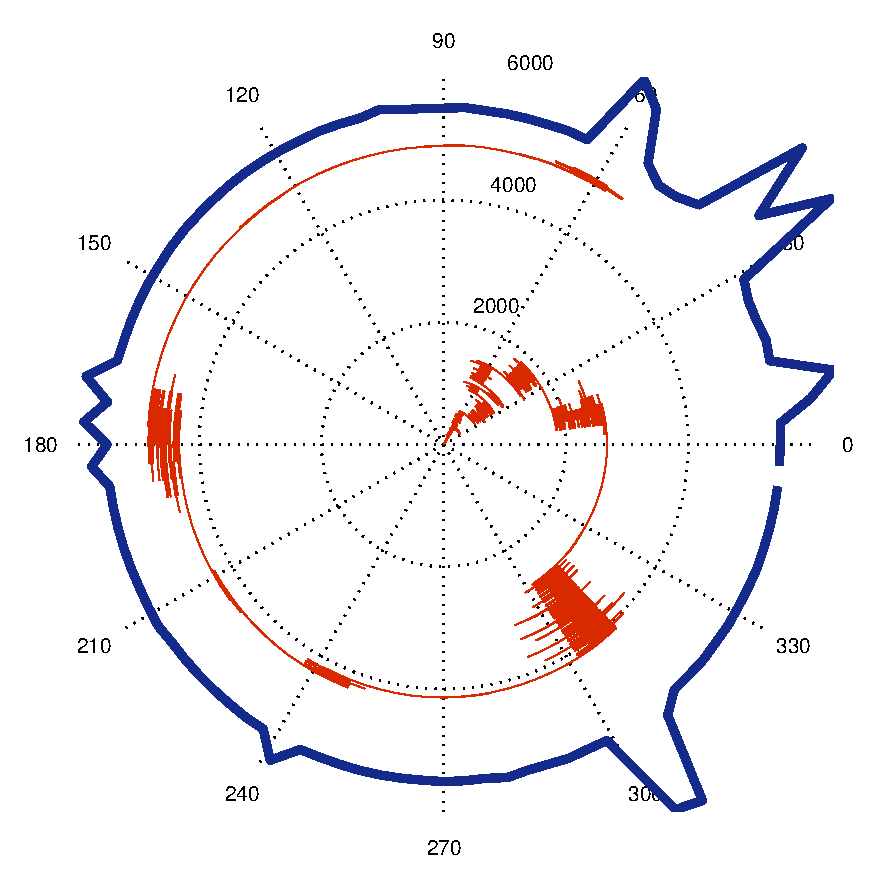
\includegraphics[height=6.5cm]{polar_1_a}
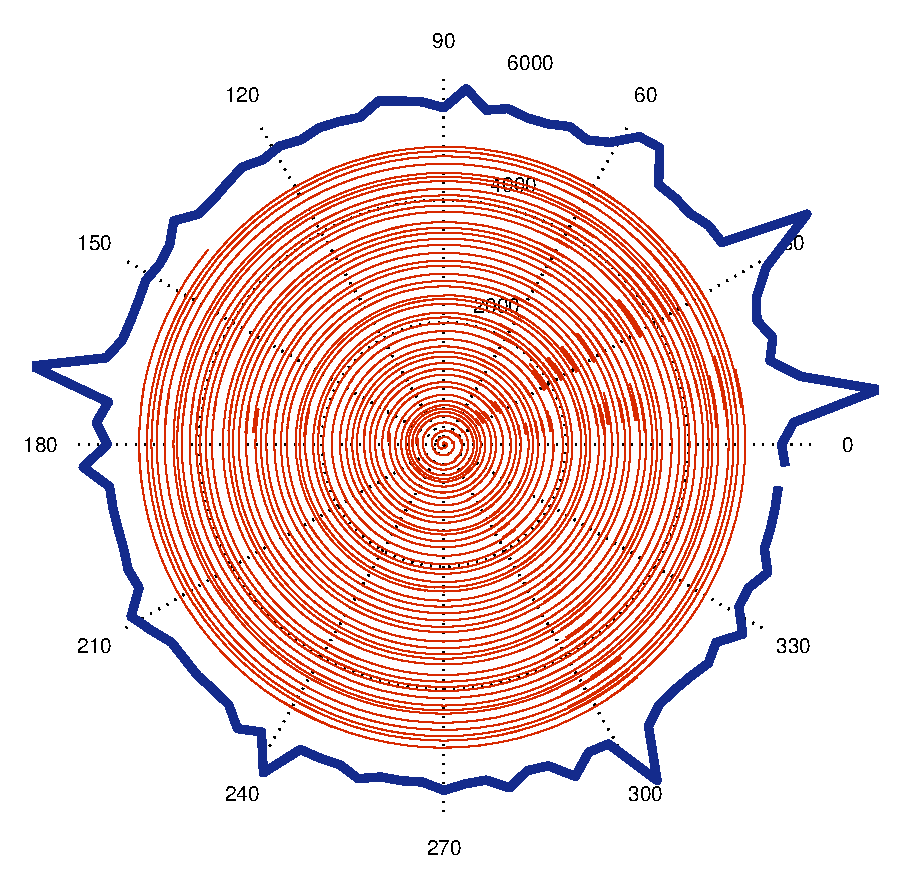
\includegraphics[height=6.5cm]{polar_2_a}

\caption{\label{traj}
Simulated trajectory of a particle on a disordered-ring.
The number of sites is $N{=}100$ and the disorder strength is $\sigma{=}5$.
The radial direction is time and the angle is the position. 
For small $s$ (top panel $s{=}0.88$) the dynamics is over-damped, 
while for large $s$ (bottom panel $s{=}2.97$) the dynamics is under-damped. 
The outer thick line the steady-state distribution (see \Ap{Ap12}). 
}
\end{figure}


% Sc vs N/M
% Sc vs alpha
%%%%%%%%%%%%%%%%%%%%%%%%%%%%%%%%%%%%%%
\begin{figure}
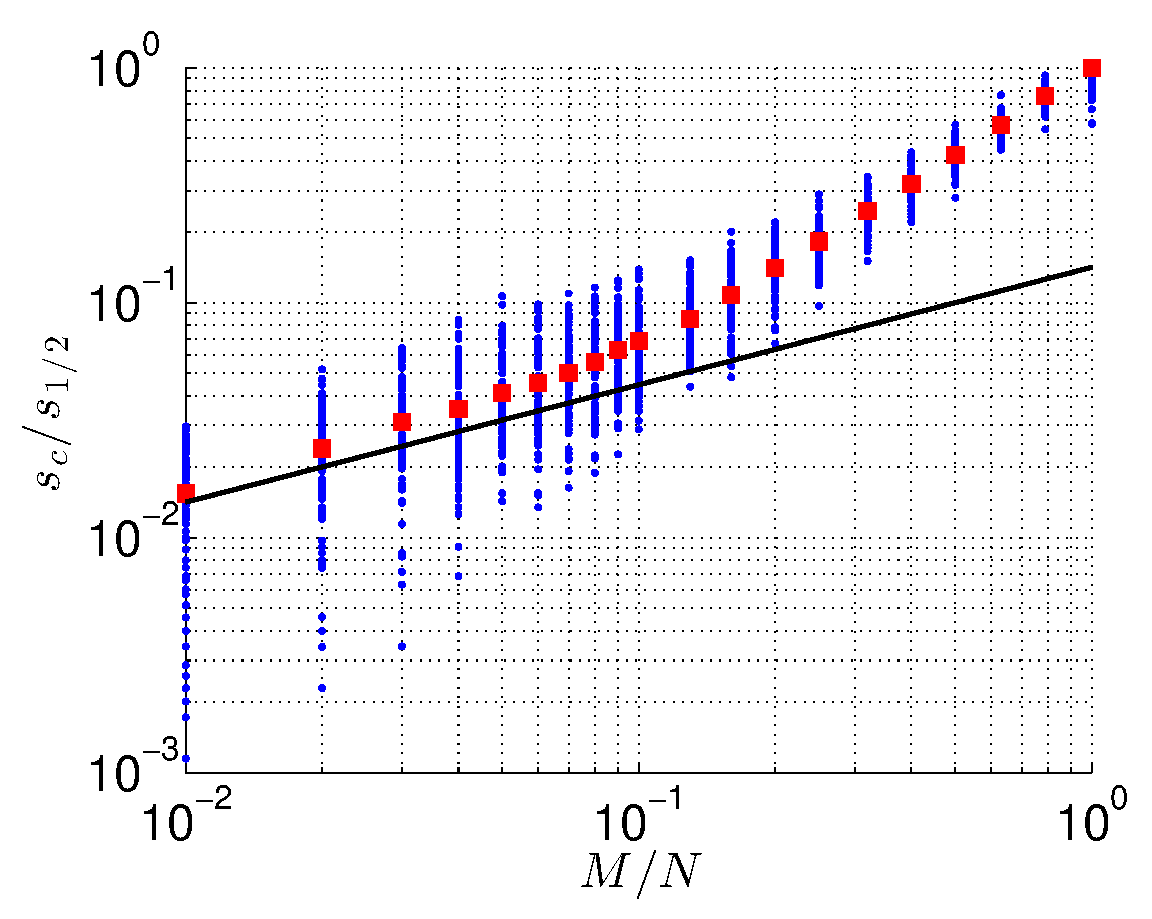
\includegraphics[height=5cm]{s_c_sparse_100_loglog}
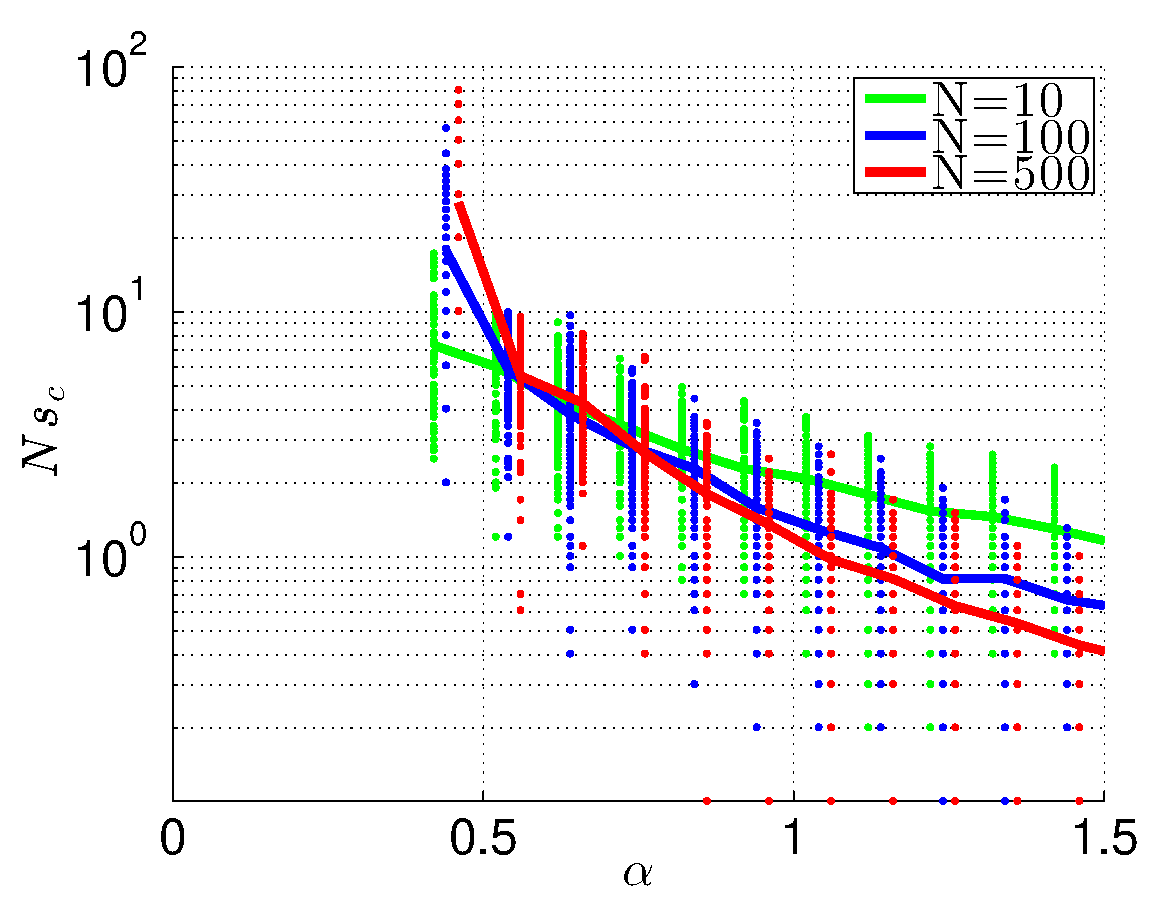
\includegraphics[height=5cm]{s_c_vs_alpha}
%
\caption{\label{sparse}
{\bf Top panel:} The threshold value $s_c$ for delocalization versus the number of stochastic field defects $M$. 
The number of sites is $N{=}100$ and the disorder strength (of the defected sites) is $\sigma{=}5$. 
Blue dots correspond to different realizations, while red dots are the average (per~$M$). 
For a fully disordered lattice we expect $s_c=s_{1/2}$, hence the scaling of the axes. 
The black line is \Eq{e33}. 
{\bf Bottom panel:} The threshold value $s_c$ versus $\alpha$. The dots are for different realizations. For $\alpha<1/2$, $s_c$ is seen to diverge, the divergence rate increases with $N$.
}
\end{figure}


% Saturation
%%%%%%%%%%%%%%%%%%%%%%%%%
\begin{figure}
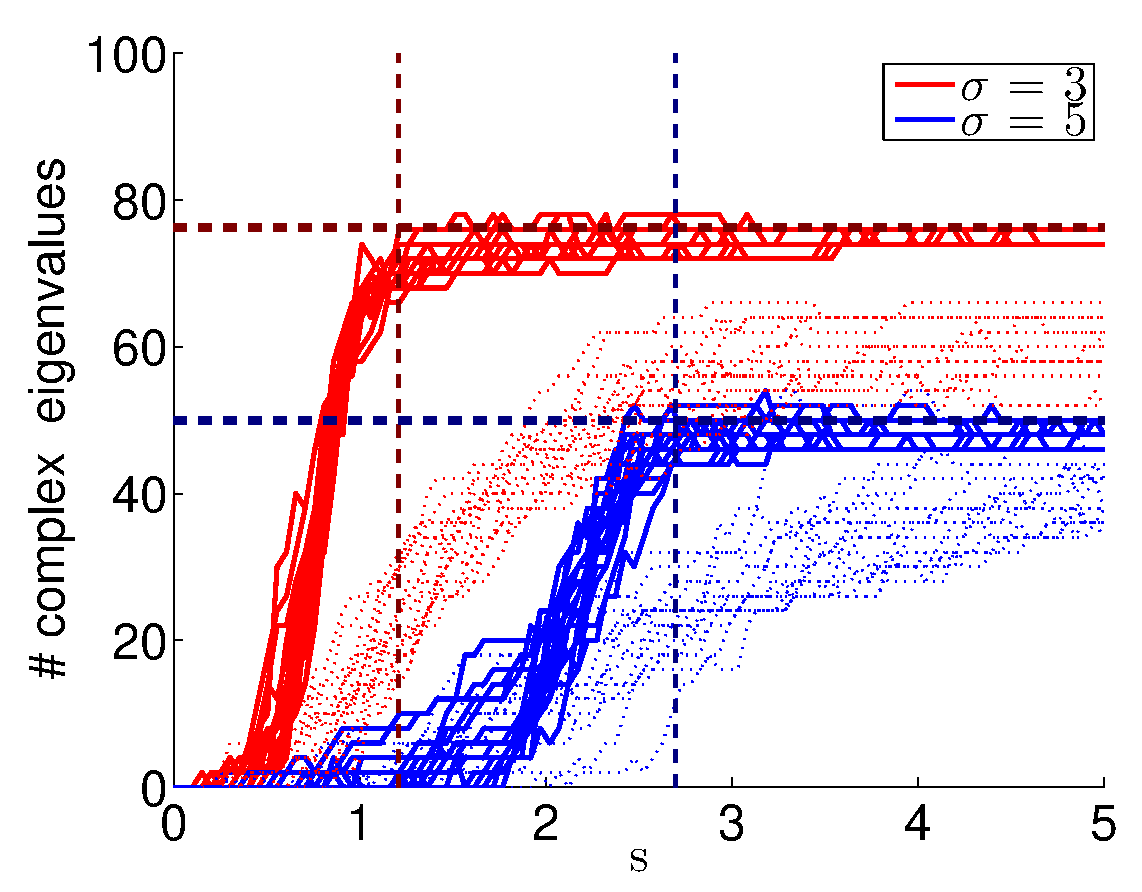
\includegraphics[height=5.4cm]{numComplex_100_alpha_sigma}


\caption{\label{figCplxSat}
The number of complex eigenvalues is counted for a ring with $N{=}100$ sites, 
for various values of the affinity~$s$. Each red line corresponds to a different
realization of field disorder with $\sigma{=}3$ (red) and $\sigma{=}5$ (blue). 
The black vertical lines are the corresponding values of~$s_1$, 
at which the sliding transition occurs. 
We see that the asymptotic fraction of complex eigenvalues saturates. 
The horizontal dashed line are the analytical estimates of \Eq{e101}. 
If the lattice were continuous with Gaussian disorder, 
the number of complex eigenvalues would go to~$100\%$.
In the background an ${\alpha=0.9}$ resistor-network disorder is shown. 
The crossover is blurred and the saturation value is lower compared to \Eq{e101}.  
}
\end{figure}







% DOS
%%%%%%%%%%%%%%%%%%%%%%%%%%%%%%
\begin{figure}
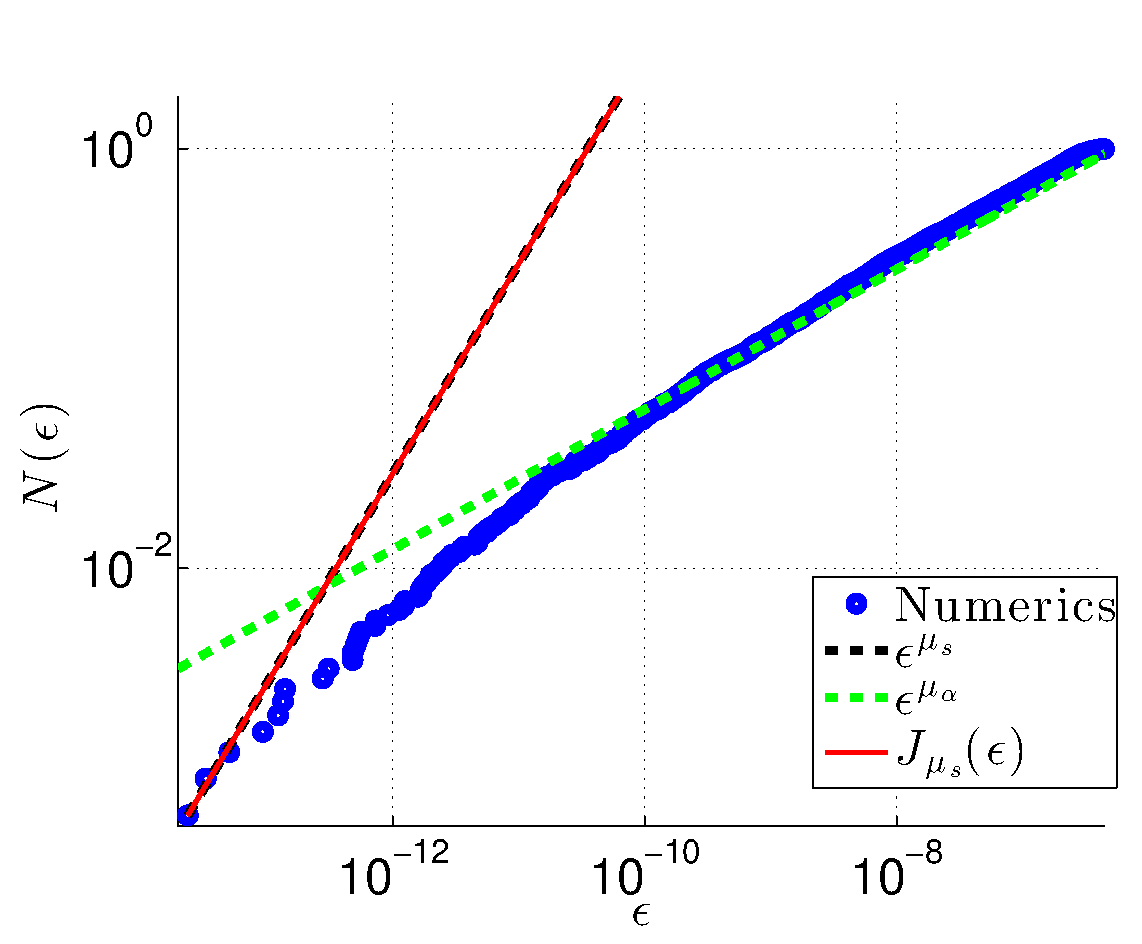
\includegraphics[height=5cm]{N_E_1_1_french.eps}

\caption{\label{fig2}\rmrk{[supplementary?]}
The integrated density of the $\epsilon_k$ for a ring with $N{=}3000$ sites. 
The system is characterized by a percolation exponent ${\mu_{\alpha} = 1/3}$, 
and by a scaled affinity ${\mu_s = 1}$. 
The stochastic-field distribution is with $\sigma{=}2$. 
The blue points are are results of numerical diagonalization. 
There is a crossover from density that corresponds to $\mu_s$ (dashed black line), 
to density that corresponds to $\mu_{\alpha}$ (dashed green line). 
}
\end{figure}


% DOS
%%%%%%%%%%%%%%%%%%%%%%%%%%%%%%5
\begin{figure}
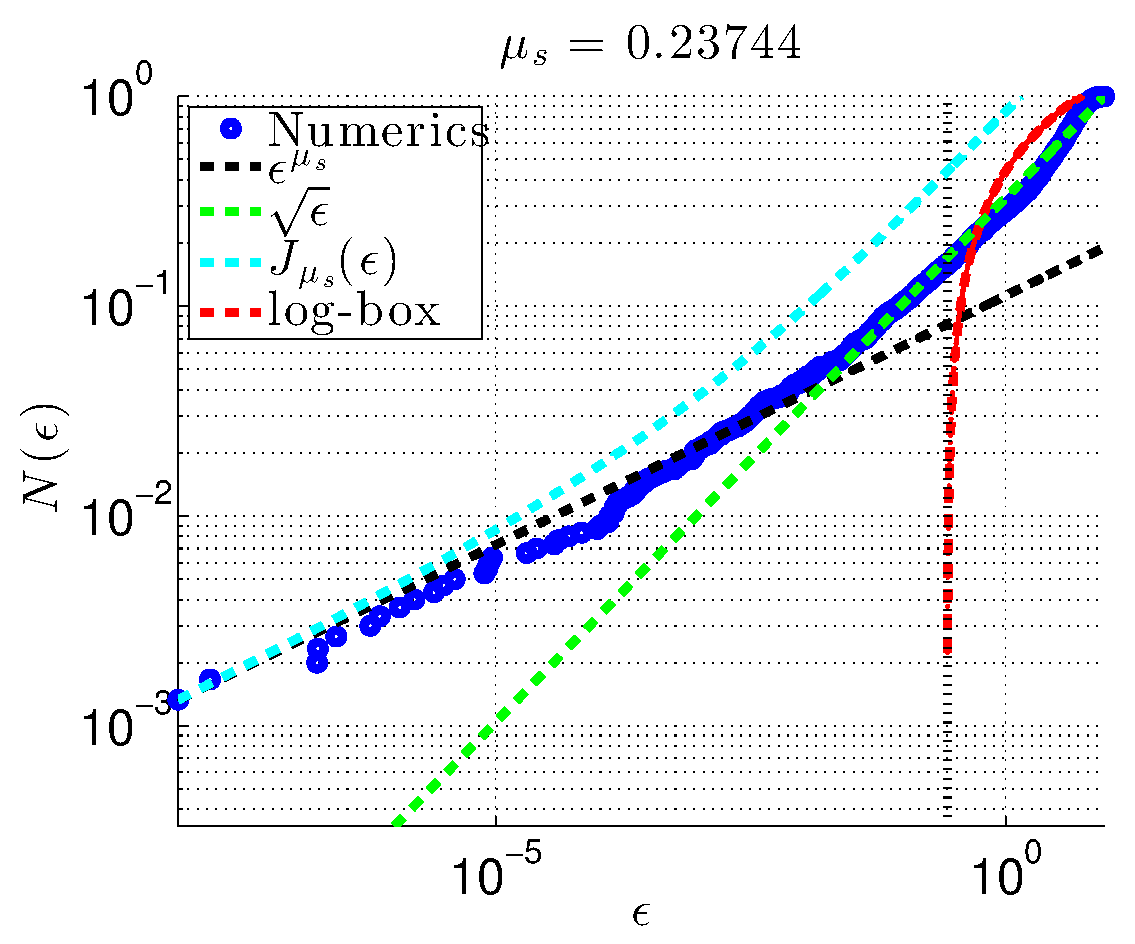
\includegraphics[height=4.5cm]{N_E_1_french}
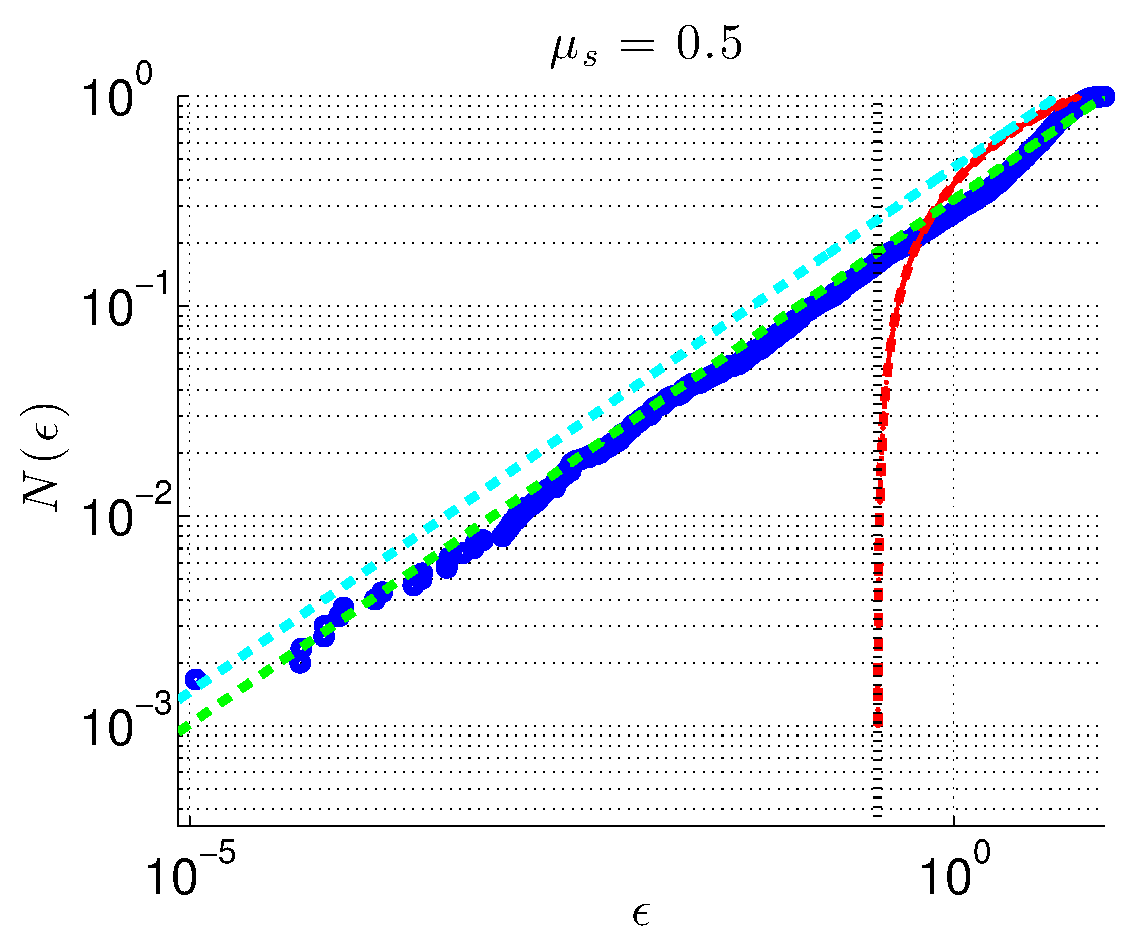
\includegraphics[height=4.5cm]{N_E_2_french}
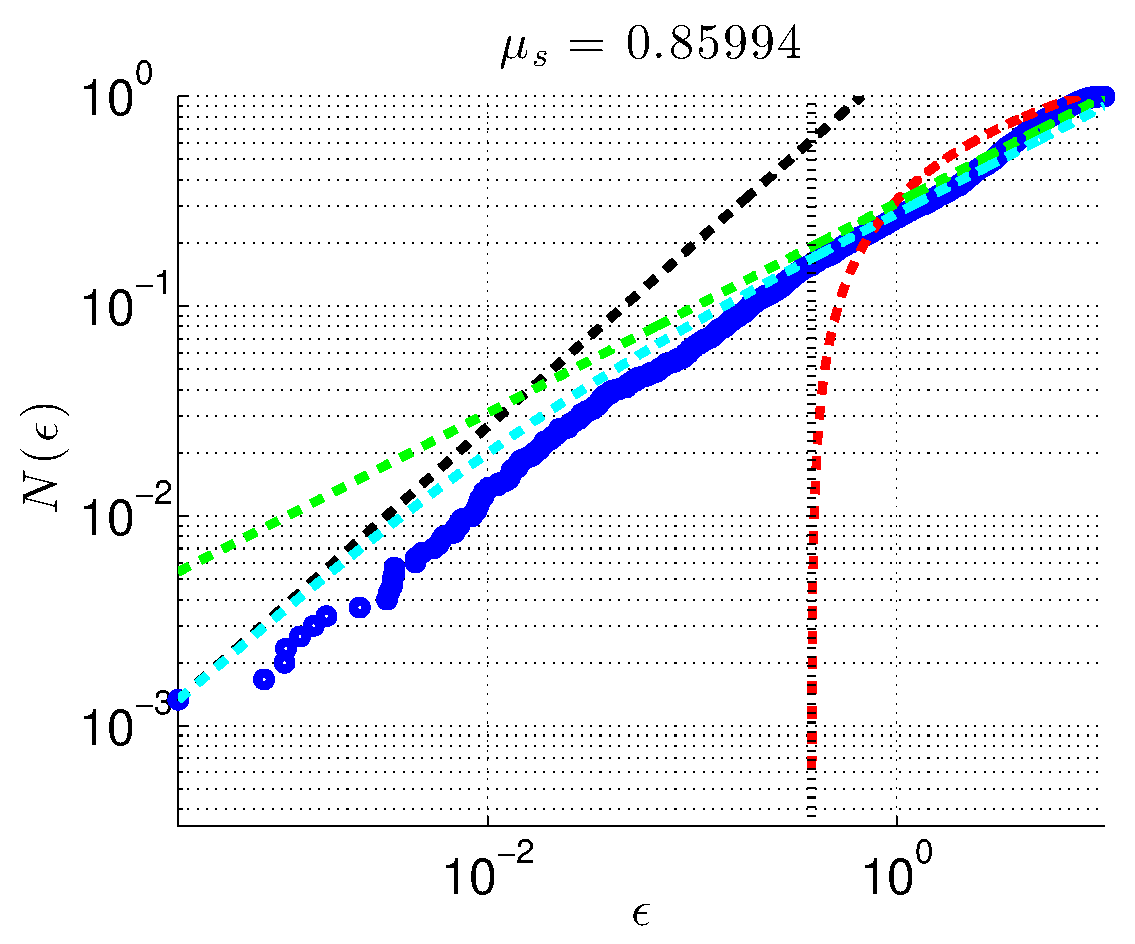
\includegraphics[height=4.5cm]{N_E_3_french}

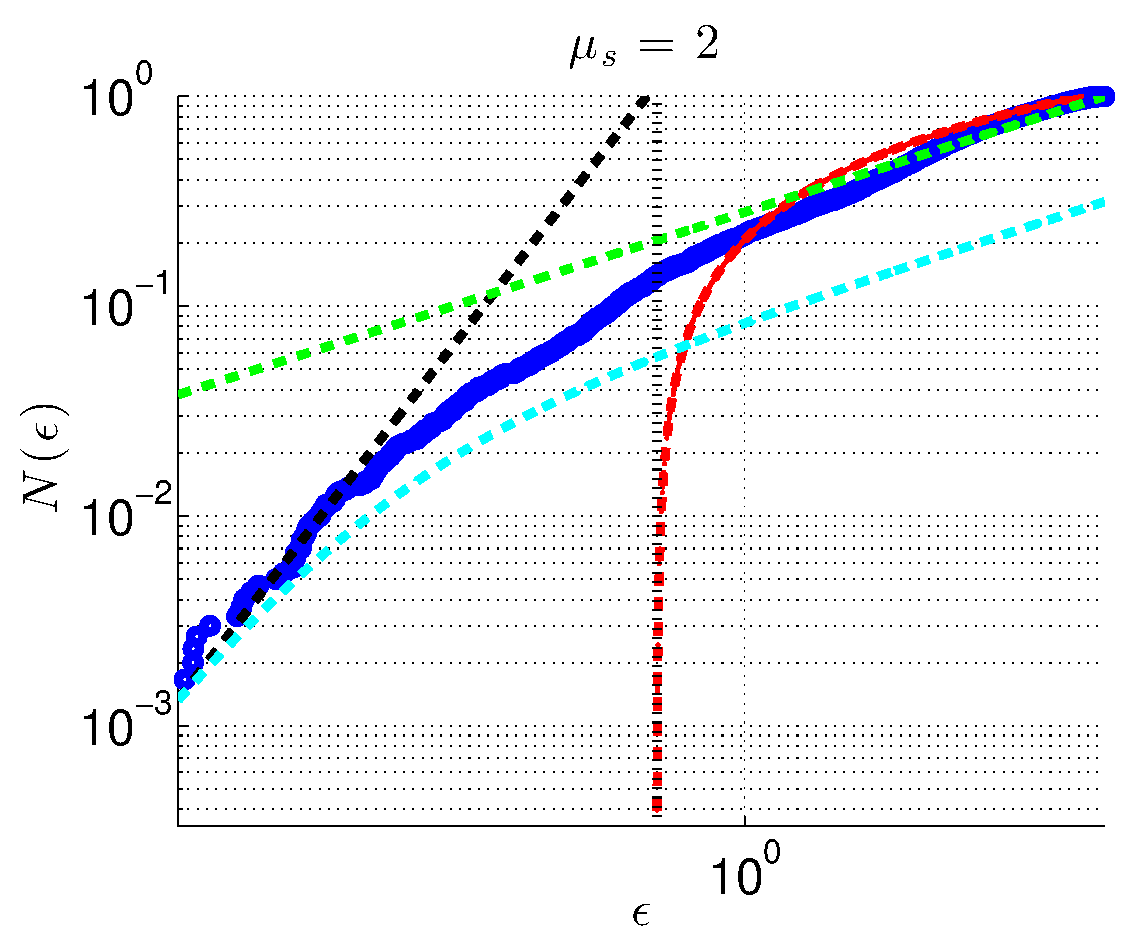
\includegraphics[height=4.5cm]{N_E_4_french}
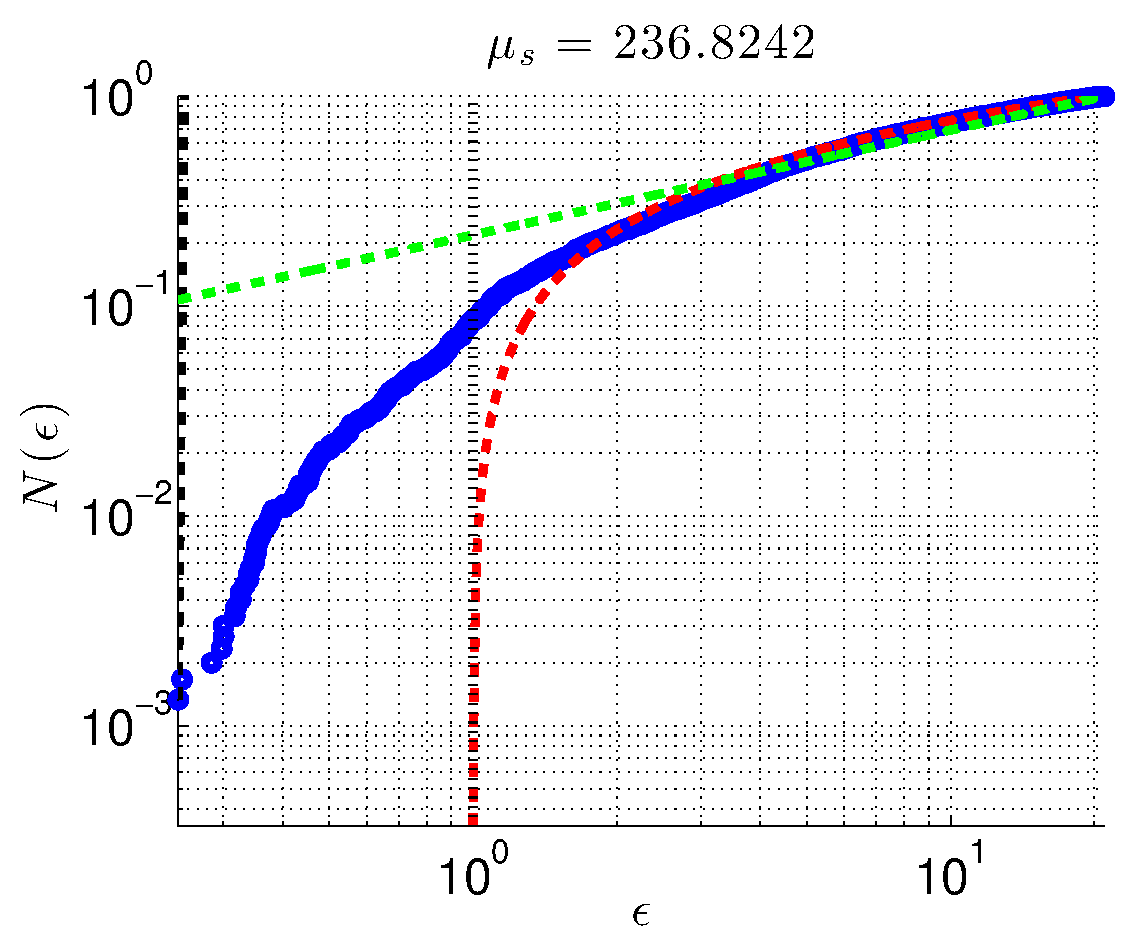
\includegraphics[height=4.5cm]{N_E_5_french}
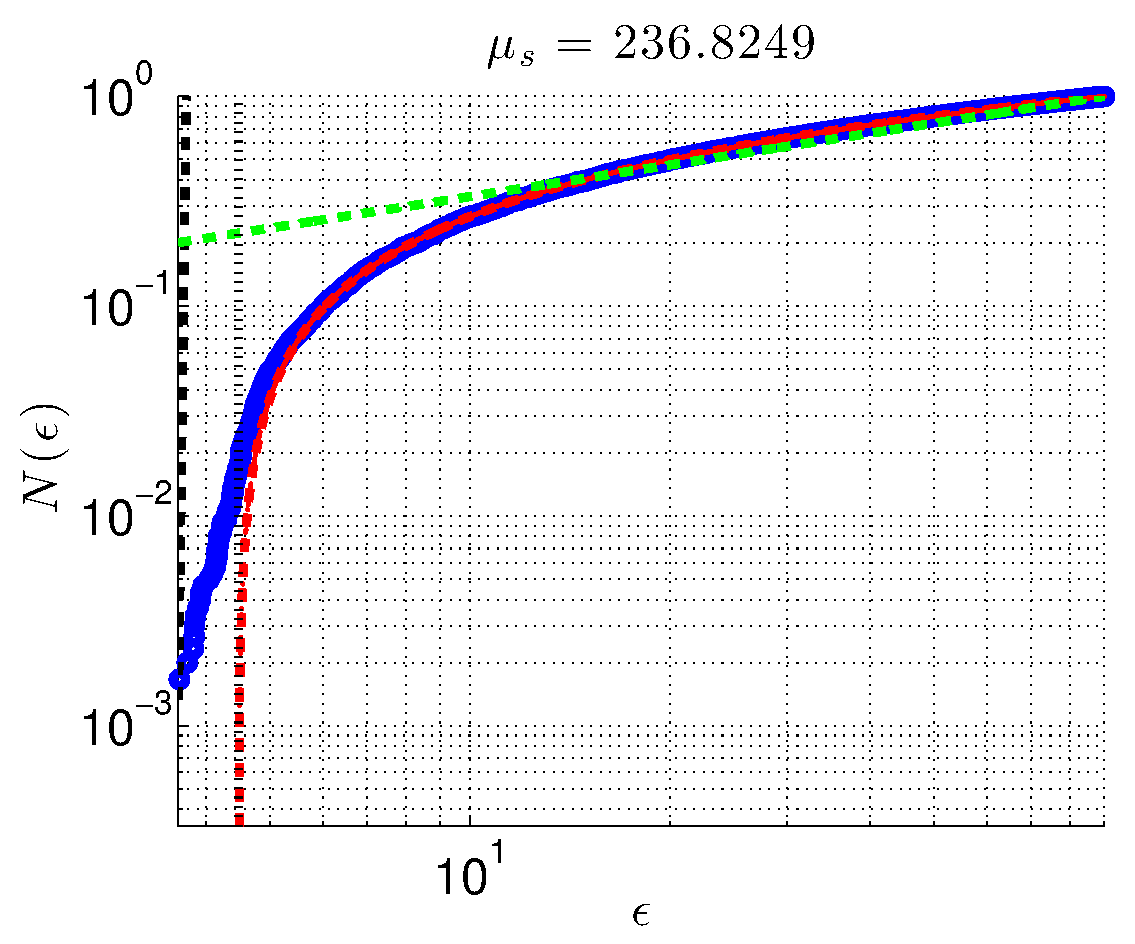
\includegraphics[height=4.5cm]{N_E_6_french}

\caption{\rmrk{[supplementary]}
The integrated density of states $N(\epsilon)$ for $N{=}3000$ ring 
with $\sigma{=}3$ and $\alpha{=}\infty$. 
The dotted vertical line is ${\epsilon_0=e^{(s-\sigma)/2}}$.
}
\end{figure}



% Complex Plane
%%%%%%%%%%%%%%%%%%%%%%%%%%%%%%%%%%%%%%%%%%%
\begin{figure}
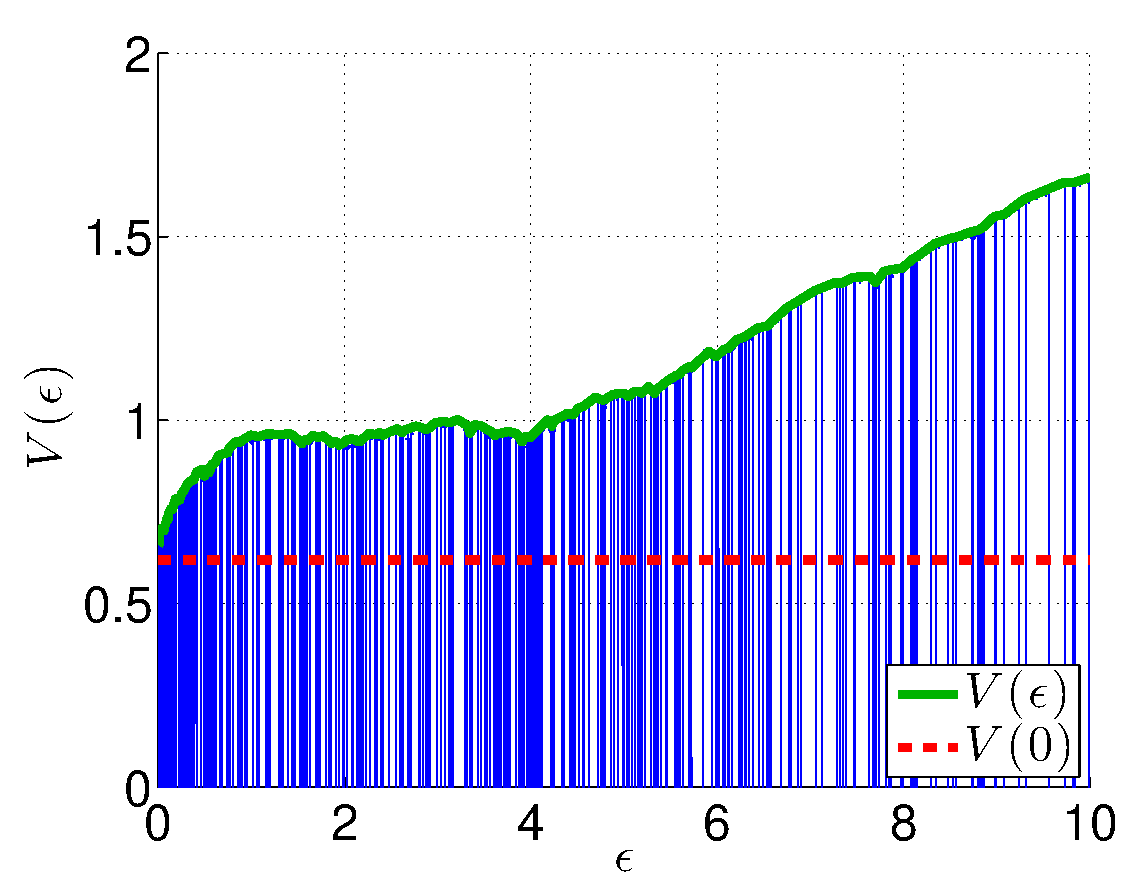
\includegraphics[height=4.5cm]{V_E_1_2b}
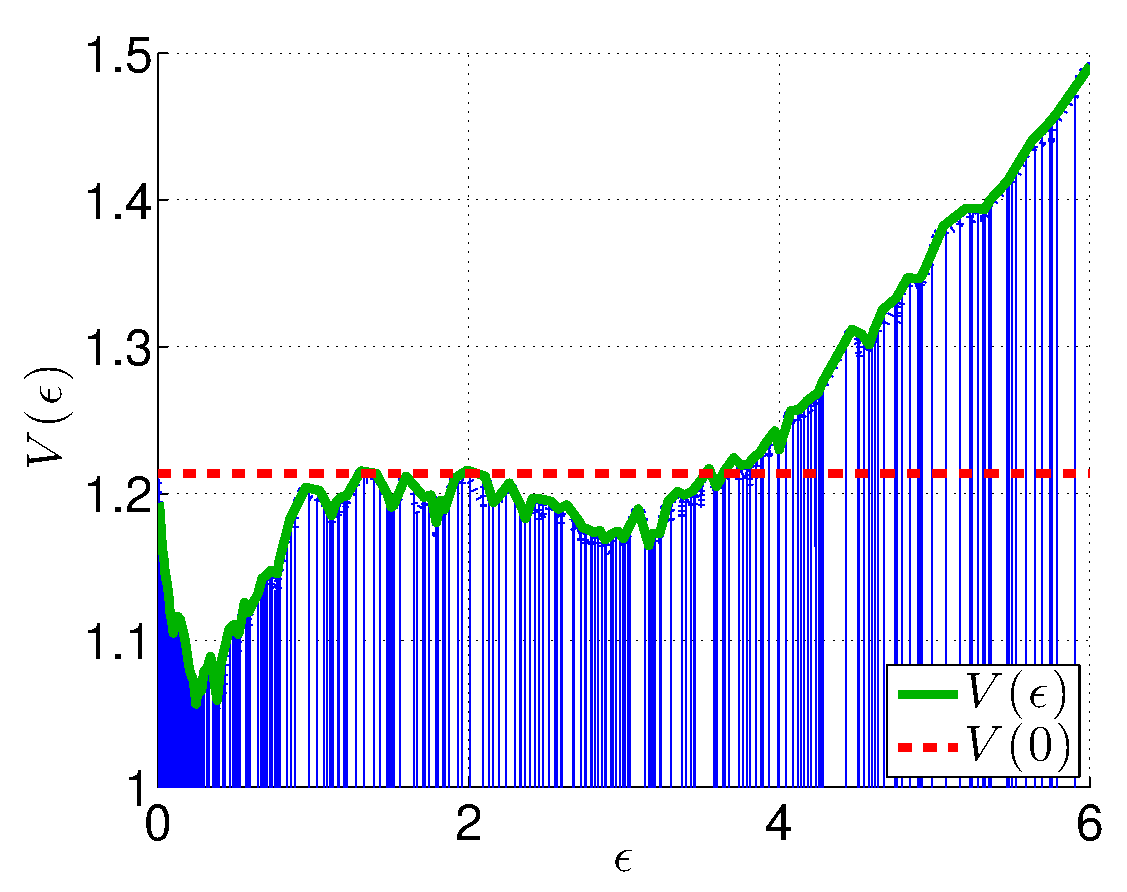
\includegraphics[height=4.5cm]{V_E_1b}
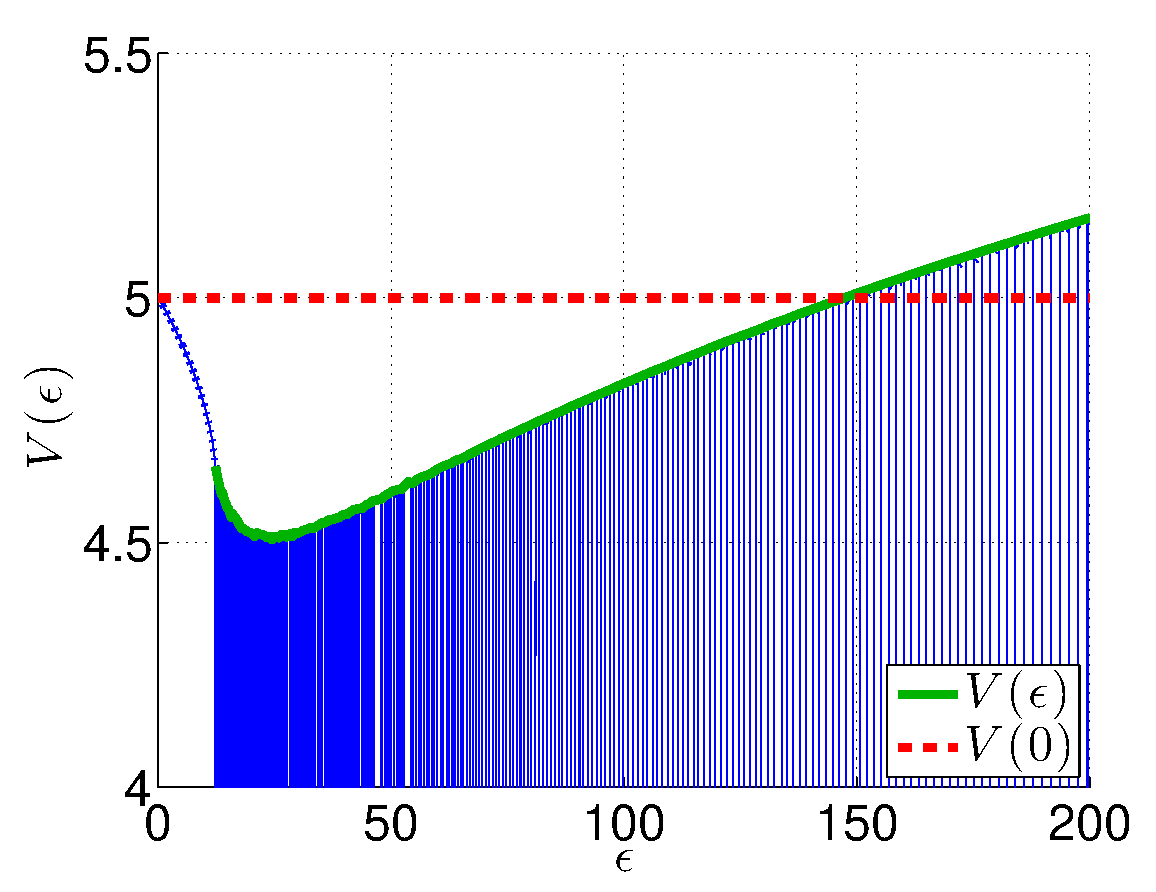
\includegraphics[height=4.5cm]{V_E_2b}

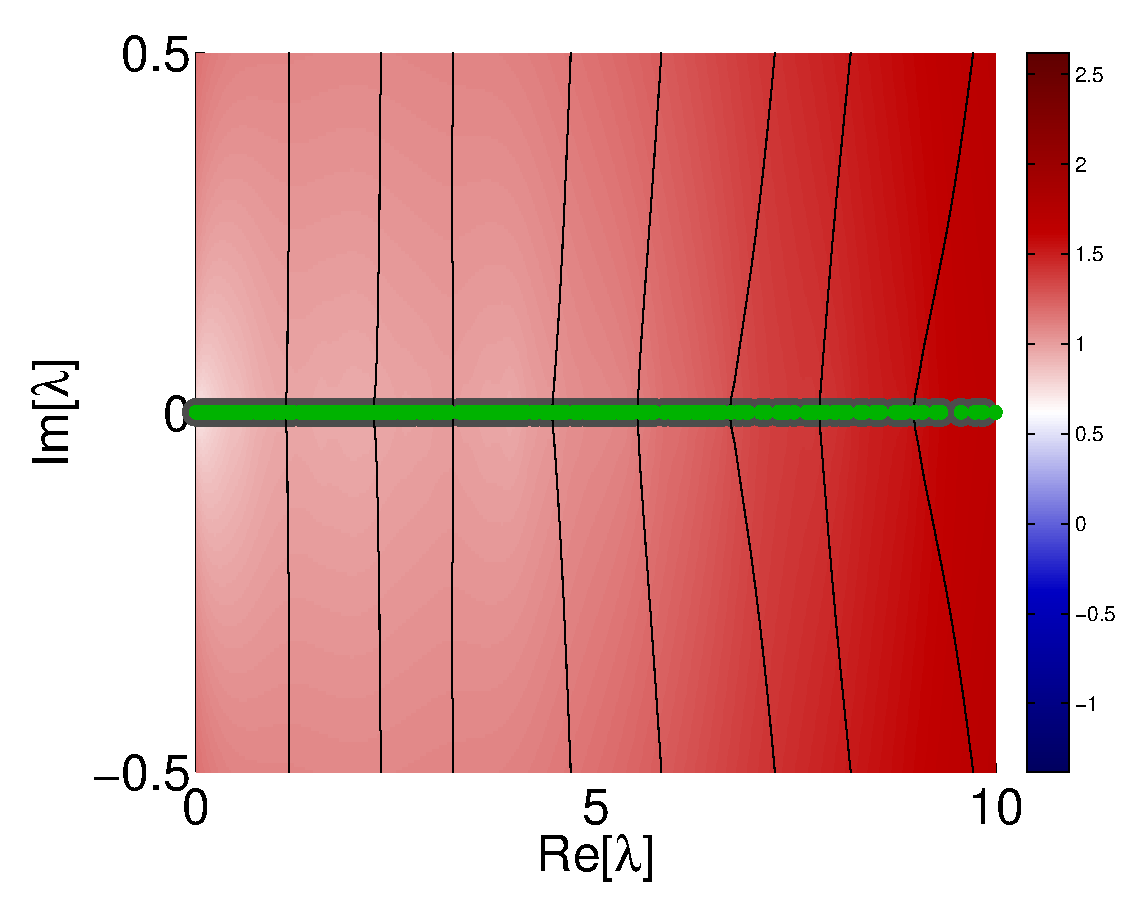
\includegraphics[height=4.5cm]{spectrum_electrostatics1_2}
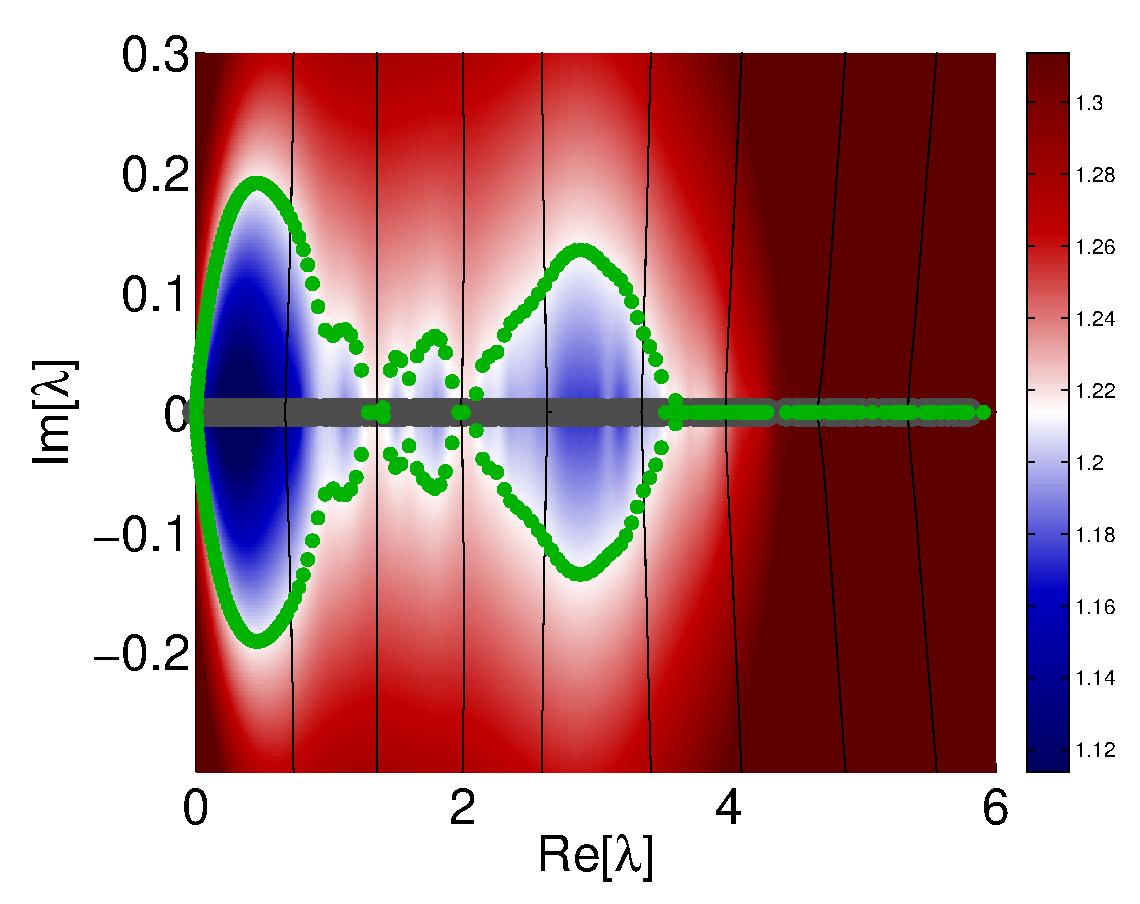
\includegraphics[height=4.5cm]{spectrum_electrostatics1}
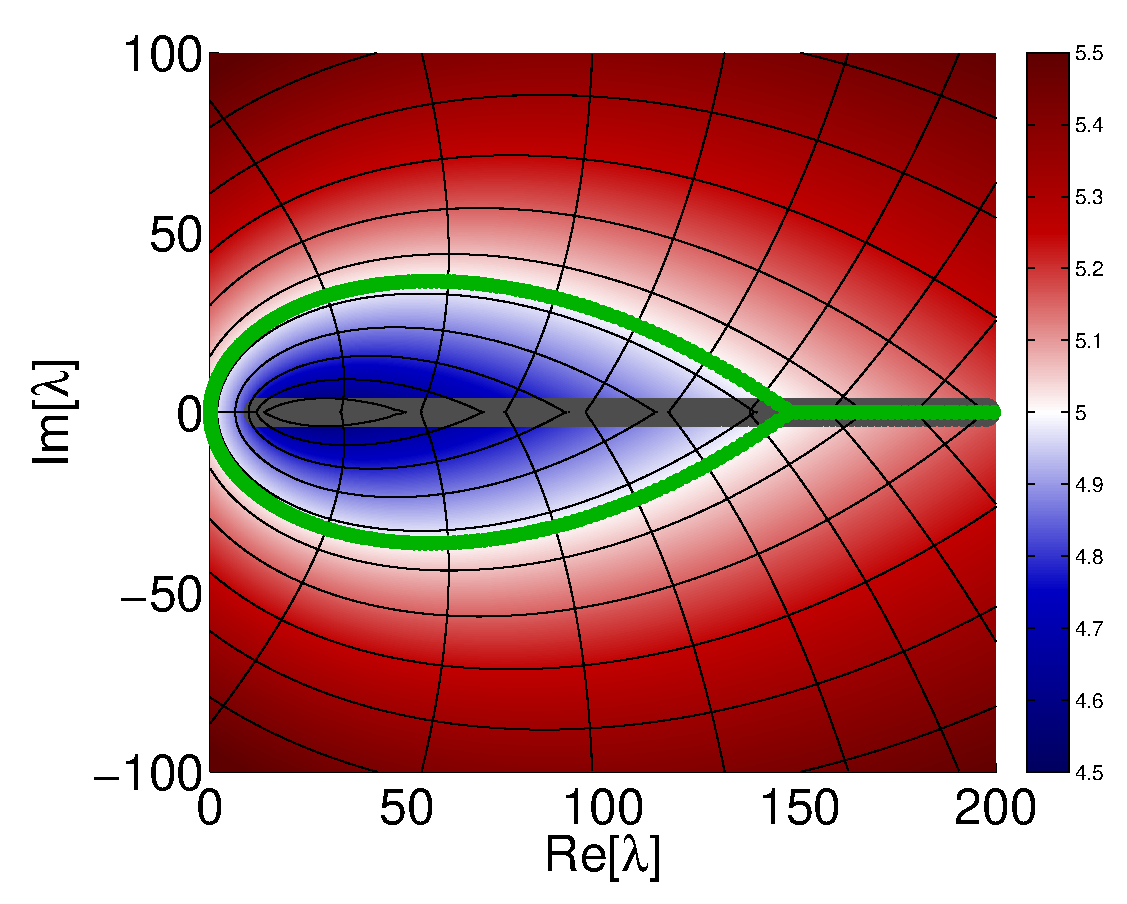
\includegraphics[height=4.5cm]{spectrum_electrostatics2}

\caption{\label{f2} \rmrk{[wide]}
The route to complexity. 
The top row shows the electrostatic potential $V(\epsilon)$ along the real axis 
and the bottom row shows the associated spectrum in the complex plane. 
The ring has $N{=}500$ sites with $\sigma{=}5$, 
and (from left to right) ${s=1.24, 2.43, 10}$. 
The expected threshold values are ${s_{1/2}=1.77}$ and ${s_1=2.7}$ and ${s_{\infty}=5}$.
In the left hand column ${s<s_{1/2}}$ and the spectrum is real.
In the middle column ${s_{1/2} < s < s_{\infty}}$ and the spectrum is  
with several complex bubbles separated by real segments. 
In the right column  ${s>s_{\infty}}$ and the real spectrum has a gap.
The complex spectrum is a fully developed complex bubble, 
tangent to the origin (no gap). 
}
\end{figure}


% Complex Plane (old)
%%%%%%%%%%%%%%%%%%%%%%%%%%%%%%%%%%%%%
\begin{figure}
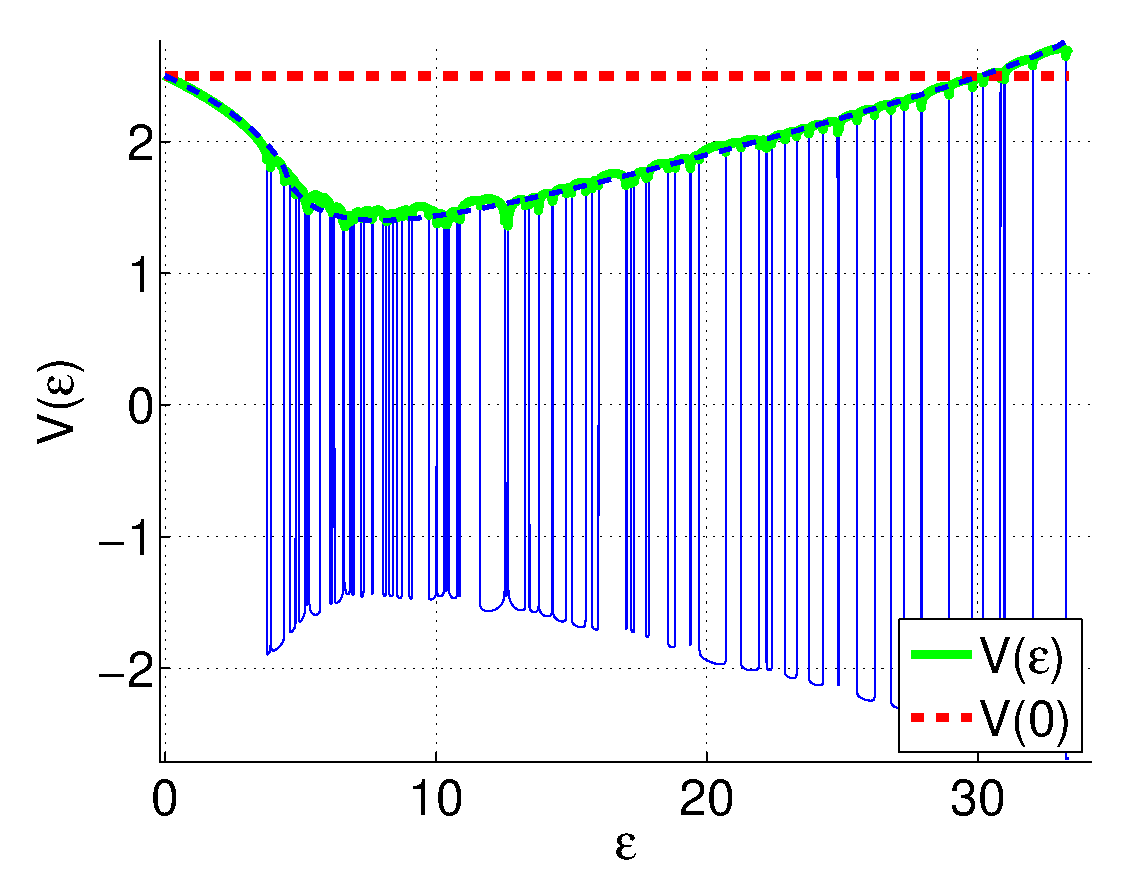
\includegraphics[width=6.2cm]{V_E_s_inf}
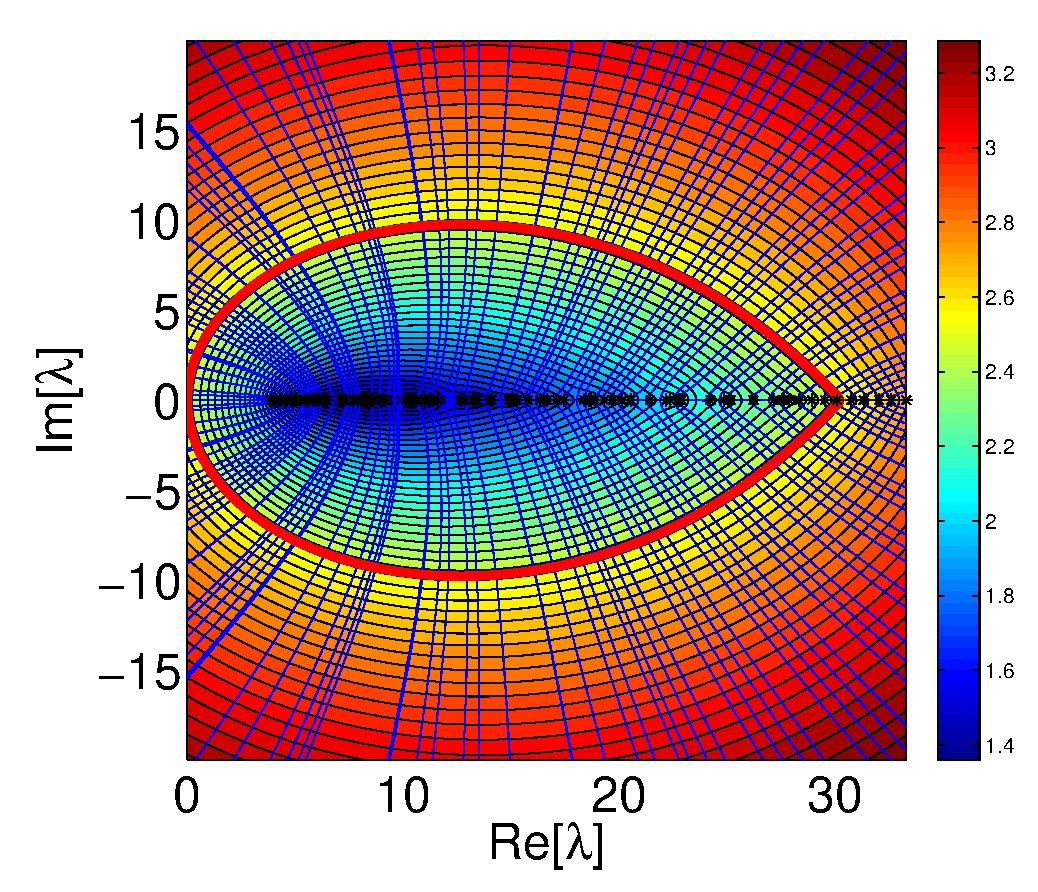
\includegraphics[width=7.5cm]{electrostatics_large_S}
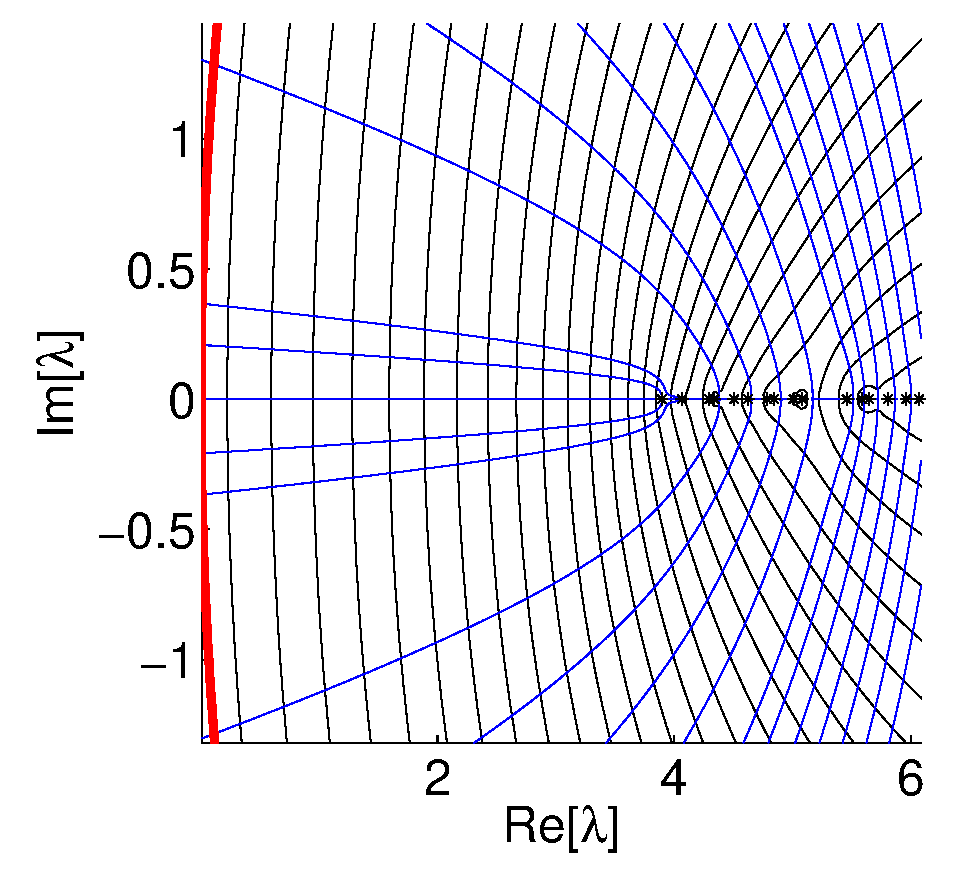
\includegraphics[width=7.5cm]{electrostatics_large_S_zoom}

\caption{\label{figWeak} \rmrk{[to be removed]}
%
{\bf Top panel}: 
The electrostatic potential $V(\epsilon)$ along the real axis. 
The dashed blue line is the analytical result assuming $\rho=N(\sigma x)^{-1}$, \Eq{e43}. 
The stars indicate the position of the "charges", 
which are the eigenvalues of the associated Hermitian matrix, $\varepsilon_j$.
%
{\bf Middle panel}: 
The electrostatic potential $\Psi(z)$ of \Eq{e22}. 
Here we consider a ring with $N=100$ sites, $\sigma=2$ and $s=5$. 
The complex $\lambda_k$ spectrum is obtained by looking 
for the intersections of the field lineswith the red thick 
equipotential line $V(z)=V(0,0)$ that goes through the origin. 
%
{\bf Bottom panel}: Zoom. 
Note that the complex spectrum unlike the real spectrum does not have a gap.
}

\end{figure}



% Step by step Electrostatics 
%%%%%%%%%%%%%%%%%%%%%%%%%%%%%%%%%%%%%%%%%
\begin{figure}[h!]
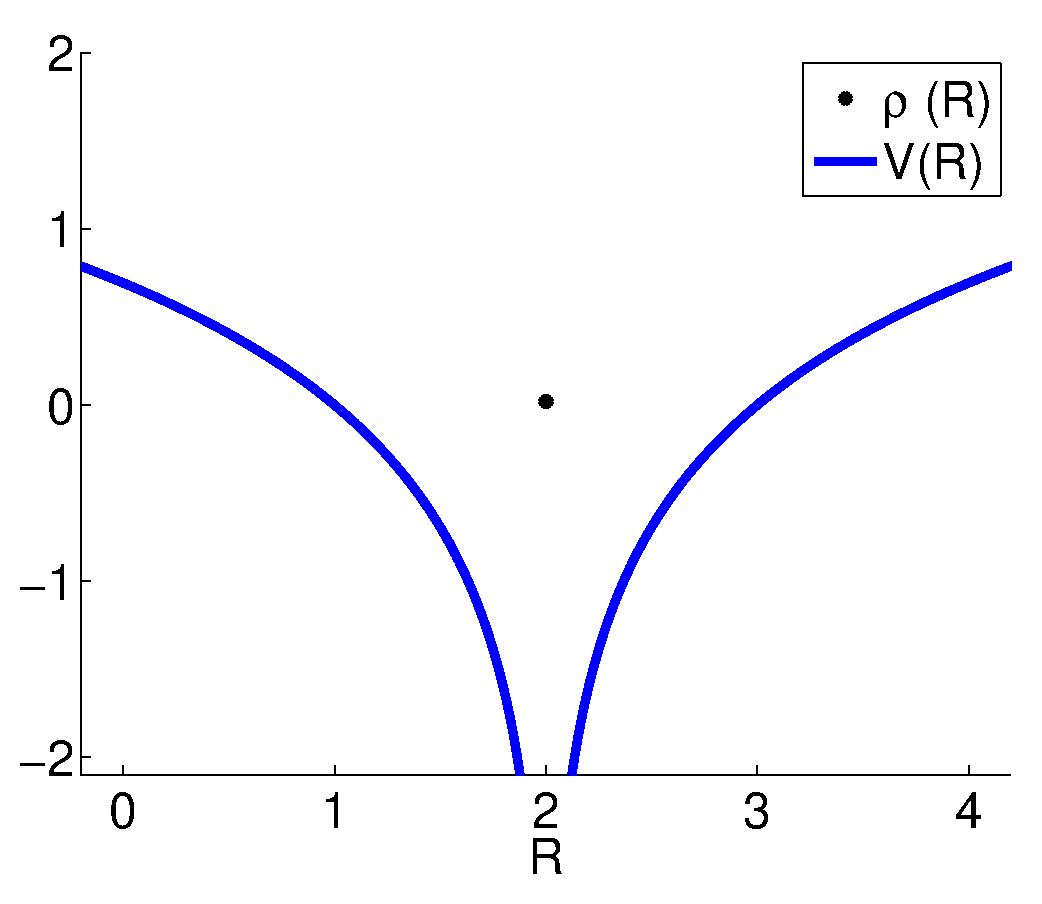
\includegraphics[height=4cm]{V_R_stepbystep_point}
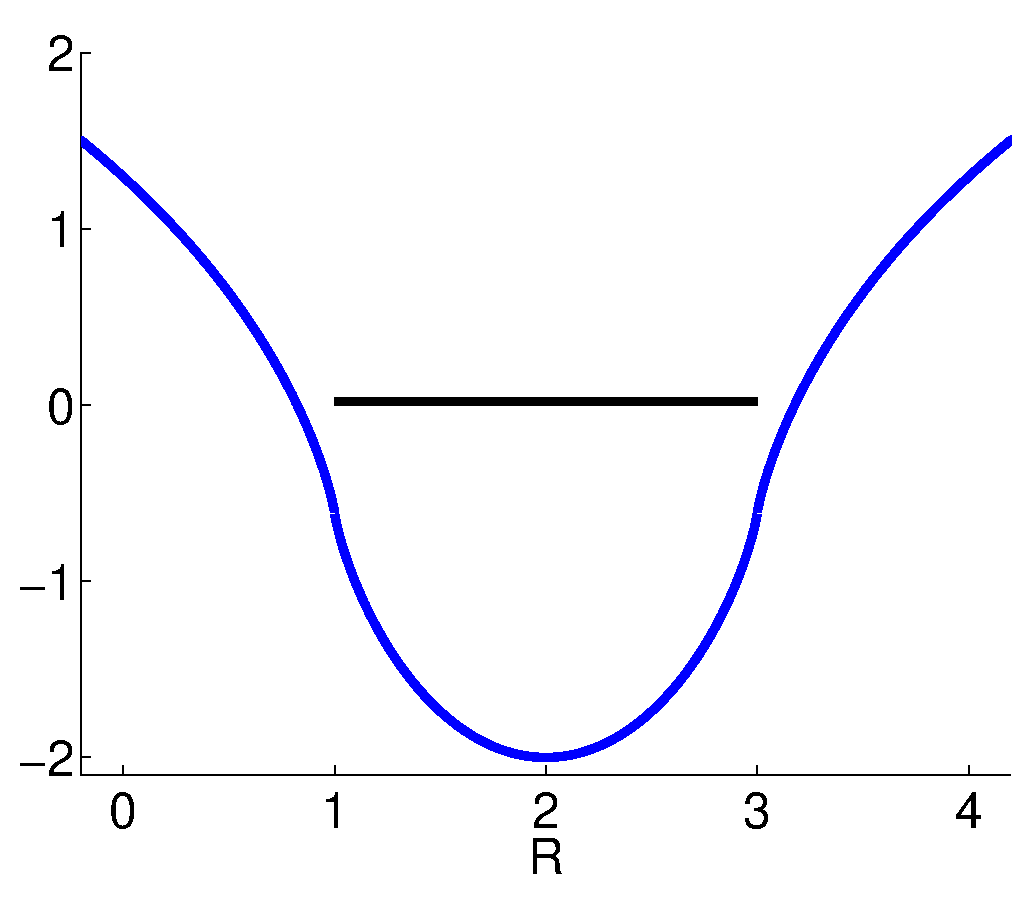
\includegraphics[height=4cm]{V_R_stepbystep_uniform}
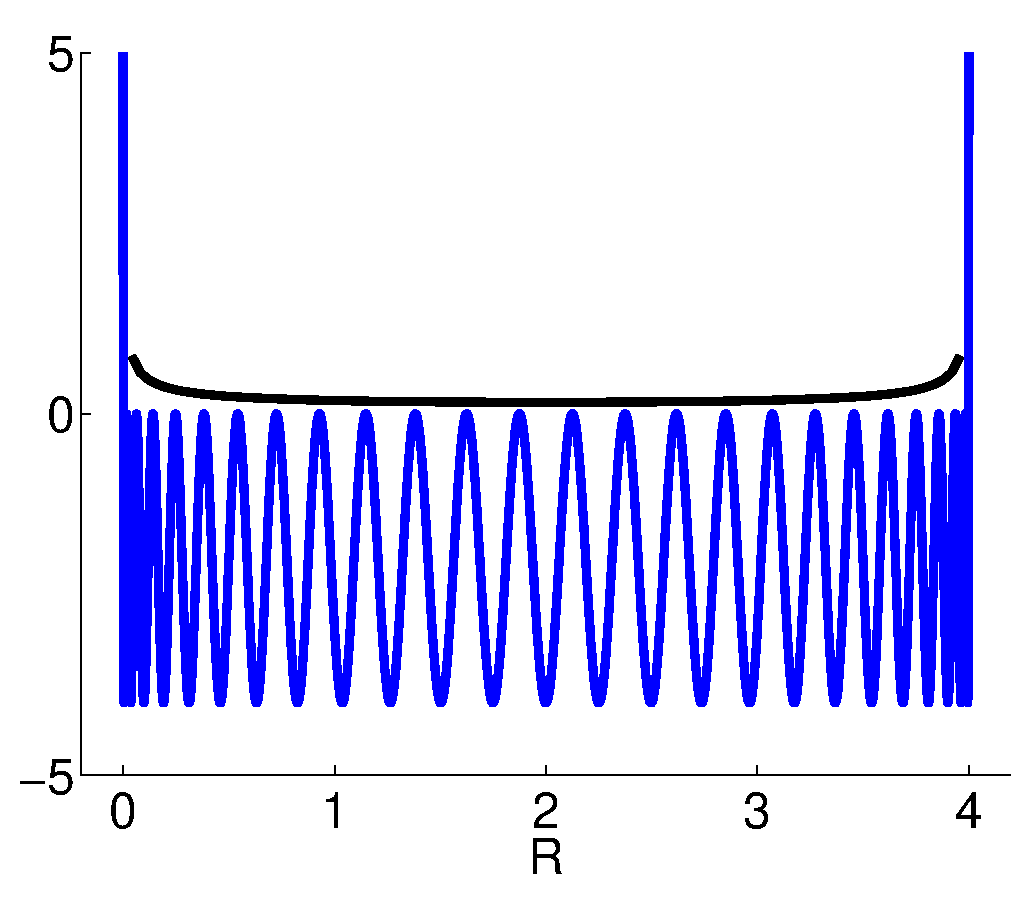
\includegraphics[height=4cm]{V_R_stepbystep_continuum}

\caption{\label{stepByStep}\rmrk{[supplementary]}
The building blocks of the electrostatic picture. 
A point charge at $R=2$ (left) generates a logarithmic potential, 
a uniform charge distribution on the interval $[1,3]$ (middle) generates a soft well
and a clean ring with $s=0$ (right) generates a flat floor (any $s\neq 0$ just shifts the charge density to the right). 
The potential is the blue line and the charge density is drawn in black.
For the clean ring we plot the spectral determinant instead of the potential, in order to show that the floor is really at zero.
}
\end{figure}



% SecularEq for clean Ring 
%%%%%%%%%%%%%%%%%%%%%%%%%%%%%%%%
\begin{figure}
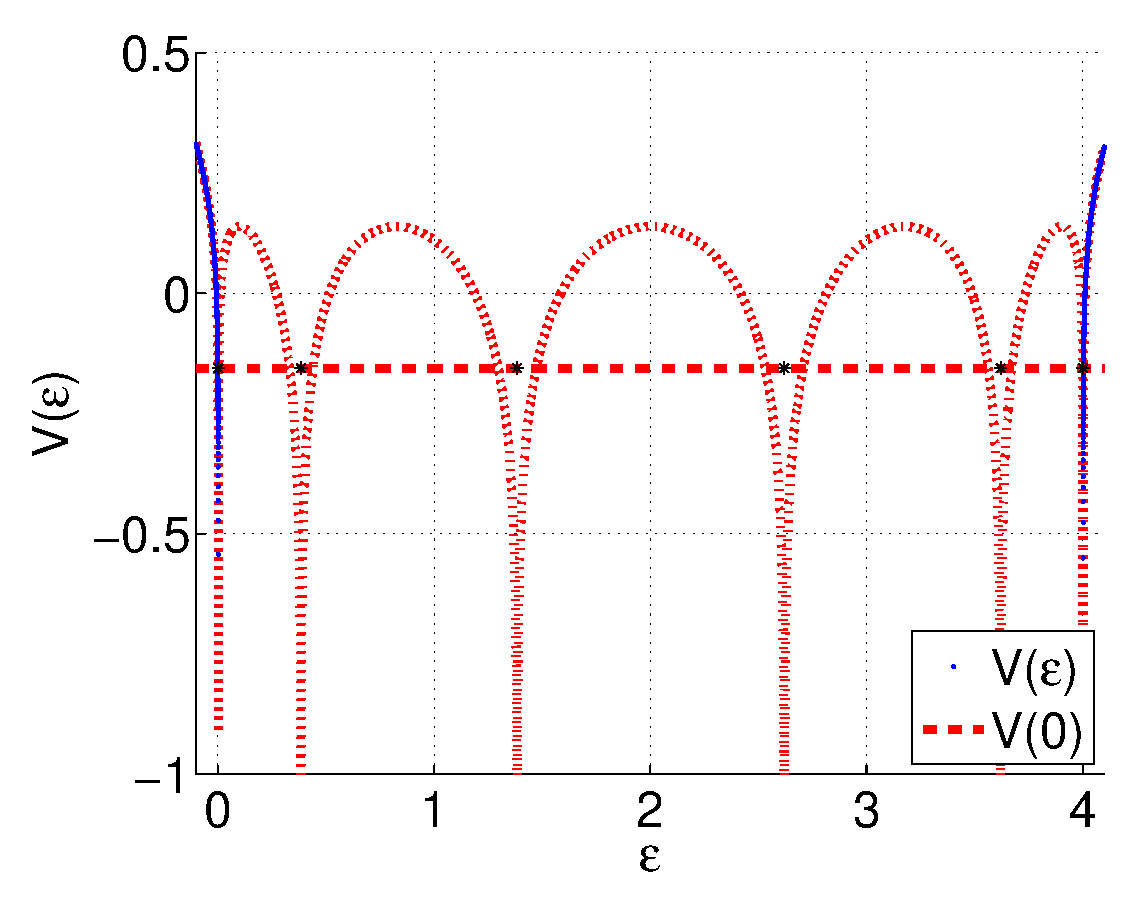
\includegraphics[height=5cm]{V_clean_1}
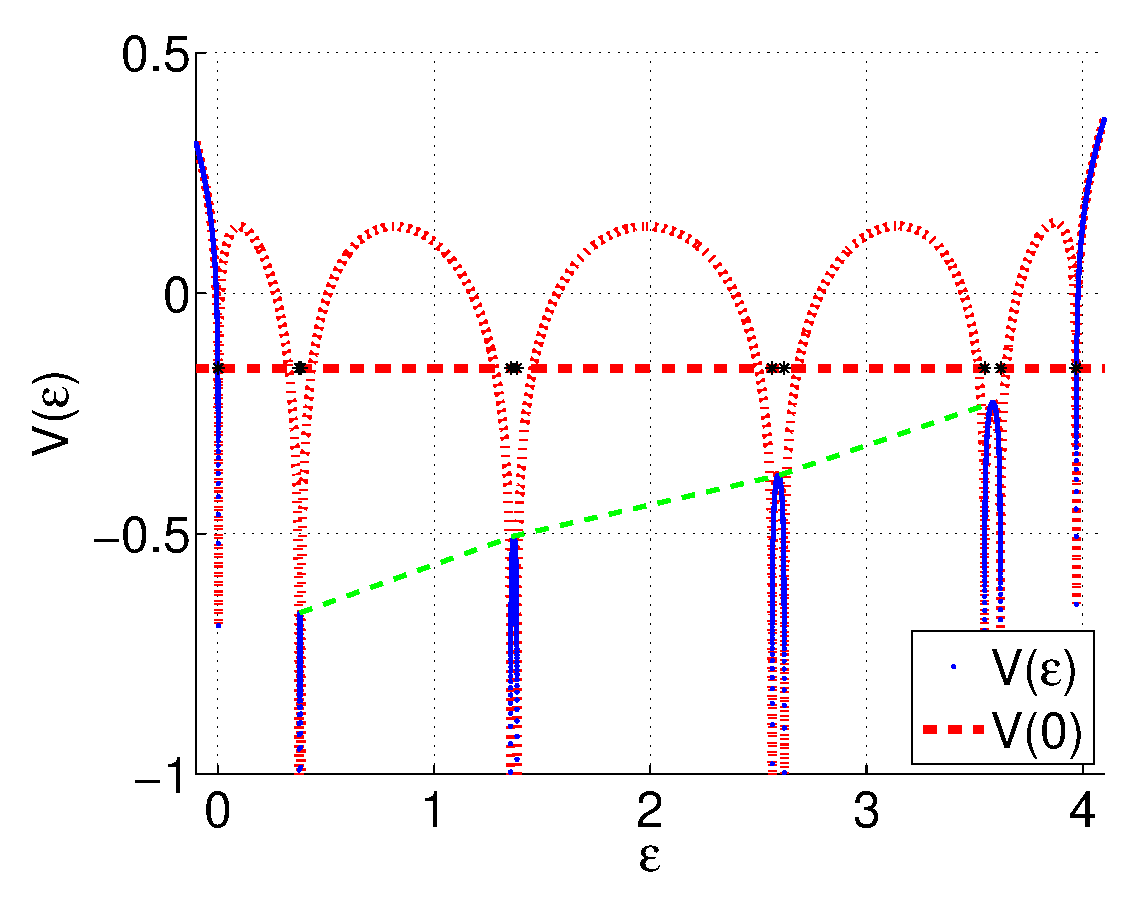
\includegraphics[height=5cm]{V_clean_2}

\caption{\label{figClean}\rmrk{[supplementary]}
Solving the secular equation for a clean ring. 
The left panel shows the electrostatic potential of a clean ring, which is doubly degenerate. 
In the right panel one of the bonds is perturbed. Here $N=10$ and $g=0.9$ and $s=0.1$
}
\end{figure}


% SecularEq for Ring with "g"
%%%%%%%%%%%%%%%%%%%%%%%%%%%%%%%
\begin{figure}
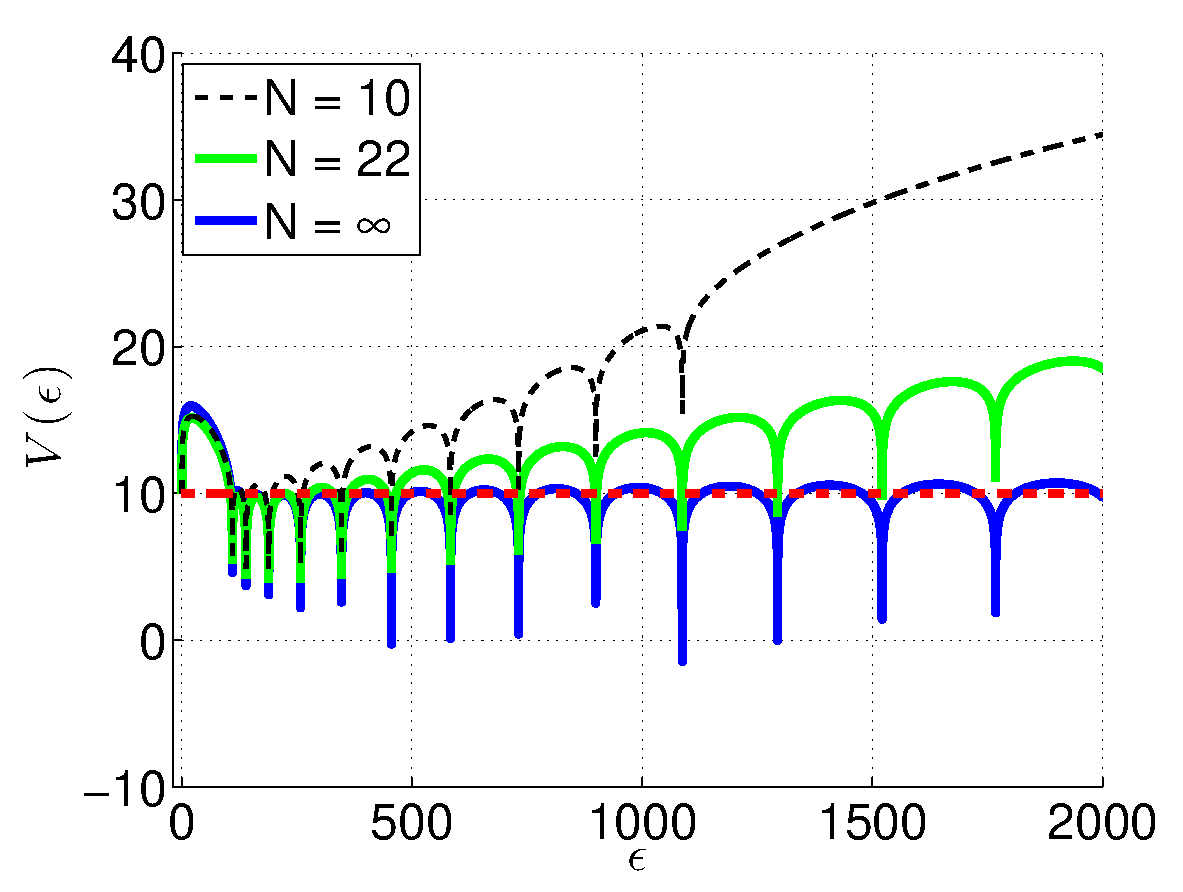
\includegraphics[height=5cm]{gRing_ES_vs_cont}
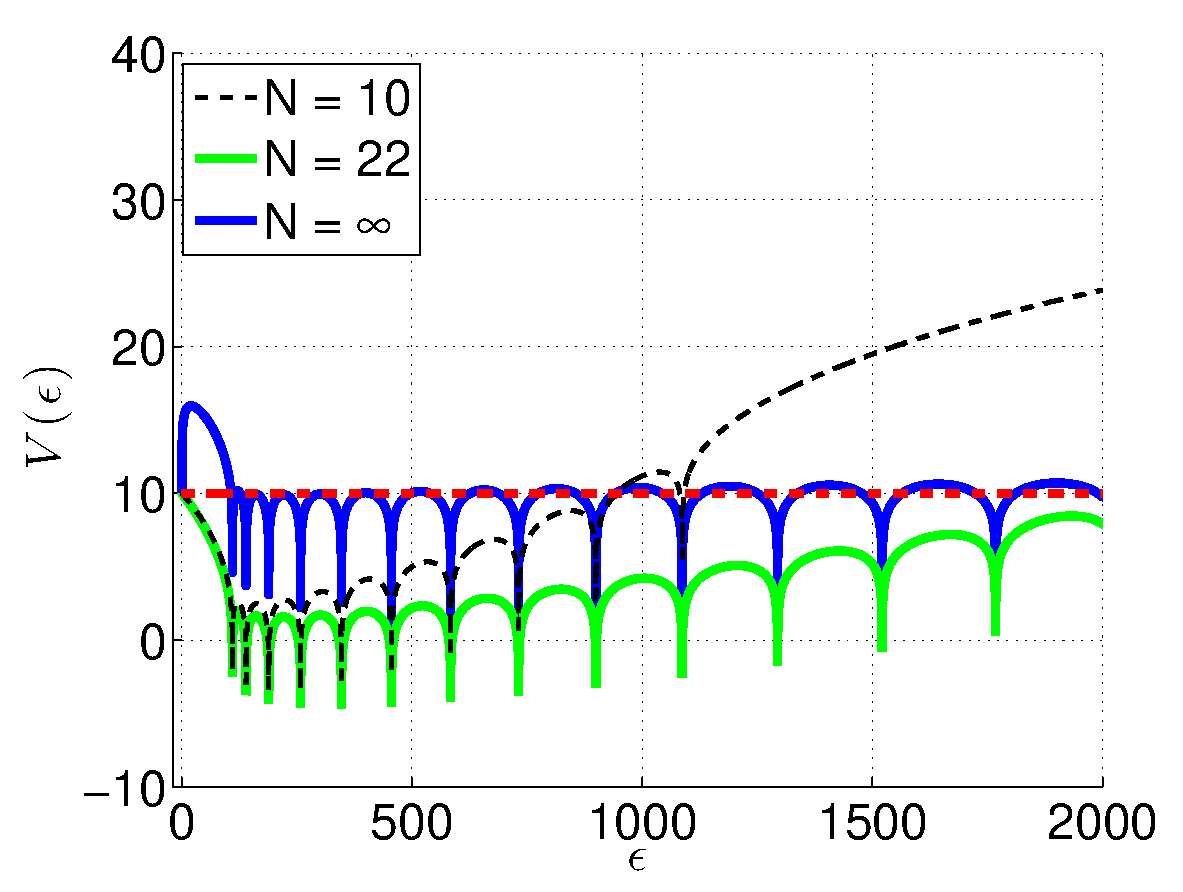
\includegraphics[height=5cm]{gRing_ES_vs_cont2}

\caption{\label{figReconstruction} \rmrk{[supplementary?]}
The secular equation of a continuous ring (solid blue) reconstructed using the electrostatic picture (green and black lines).
On the left panel the charge at the origin is included, while on the right it is not. 
The dashed red horizontal line is $V(0)=\ln(2\cosh(S/2)-2)$.
The charge at the origin is essential to determine the low energy behavior 
(On the left panel there is good agreement of the blue and green lines along the first few oscillations) , 
while the linear trend that appears in the electrostatic reconstruction is due to finite size truncation (as the number of charges is increased, the slope becomes smaller). 
For this figure, ${L=1, \ G=10^{-3}, \ s=20}$.
}
\end{figure}


% Gamma
%%%%%%%%%%%%%%%%%%%%%%%%%%%
\begin{figure}
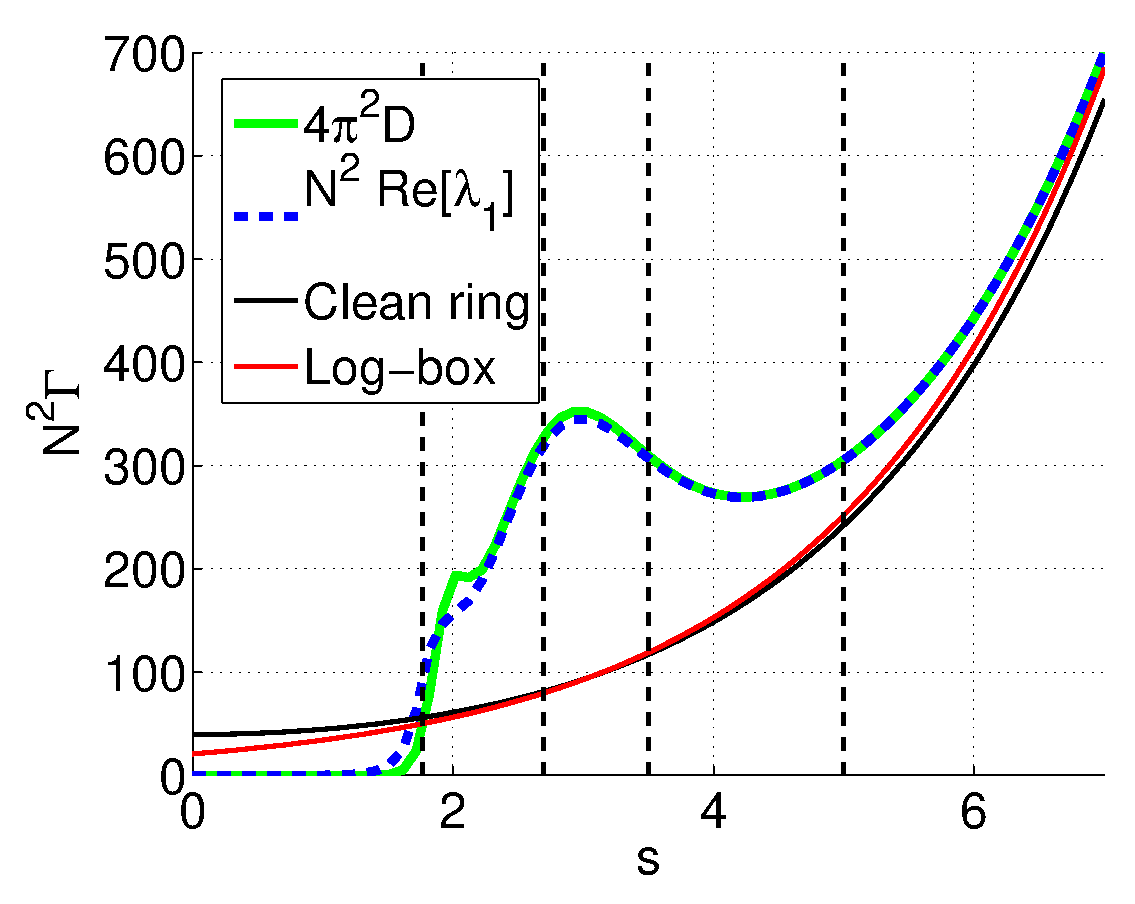
\includegraphics[height=6cm]{gap_D_sigma5_N_1000}

\caption{\label{f1}
The relaxation rate $\Gamma$ versus the affinity $s$ for $N{=}1000$ sites and $\sigma{=}5$. 
The non monotonic dashed blue line has been obtained via numerical diagonalization, 
whereas the solid green was obtained by calculating the diffusion coefficient as in \cite{nes}.
The monotonic lines are the clean-ring \Eq{e13} (black) and large-bias \Eq{e52} (red) estimates. 
The vertical dashed lines are the thresholds $s_{\mu}$ 
that are associated with ${\mu= 1/2, \ 1, \ 2, \ \infty}$ (from left to right).
}
\end{figure}





%%%%%%%%%%%%%%%%%%%%%%%%%%%%%%%%%%%%%%%%%%%%%%%%%%%%%%%%%%%%%%%%%%%%%%%%%%%%%%%%%%%%
%%%%%%%%%%%%%%%%%%%%%%%%%%%%%%%%%%%%%%%%%%%%%%%%%%%%%%%%%%%%%%%%%%%%%%%%%%%%%%%%%%%%
%%%%%%%%%%%%%%%%%%%%%%%%%%%%%%%%%%%%%%%%%%%%%%%%%%%%%%%%%%%%%%%%%%%%%%%%%%%%%%%%%%%%
%%%%%%%%%%%%%%%%%%%%%%%%%%%%%%%%%%%%%%%%%%%%%%%%%%%%%%%%%%%%%%%%%%%%%%%%%%%%%%%%%%%%
\clearpage
\bibliography{neg.bib}{}
%\bibliographystyle{ieeetr}


%%%%%%%%%%%%%%%%%%%%%%%%%%%%%%%%%%%%%%%%%%%%%%%%%%%%%%%%%%%%%%%%%%%%%%%%%%
%%%%%%%%%%%%%%%%%%%%%%%%%%%%%%%%%%%%%%%%%%%%%%%%%%%%%%%%%%%%%%%%%%%%%%%%%%

\section*{Acknowledgements}

This research has been supported by  by the Israel Science Foundation (grant No. 29/11).


\hidea{
\section*{Author contributions statement}

Both authors have contributed to this article. 

\section*{Additional information} 

% Reprints and permissions information is available at www.nature.com/reprints\\
The authors declare that they have no competing financial interests.
% Correspondence and requests for materials should be addressed to avardi@bgu.ac.il or dcohen@bgu.ac.il
}





%%%%%%%%%%%%%%%%%%%%%%%%%%%%%%%%%%%%%%%%%%%%%%%%%%%%%%%%%%%%%%%%%%%%%%%%%%
%%%%%%%%%%%%%%%%%%%%%%%%%%%%%%%%%%%%%%%%%%%%%%%%%%%%%%%%%%%%%%%%%%%%%%%%%%
%%%%%%%%%%%%%%%%%%%%%%%%%%%%%%%%%%%%%%%%%%%%%%%%%%%%%%%%%%%%%%%%%%%%%%%%%%
%%%%%%%%%%%%%%%%%%%%%%%%%%%%%%%%%%%%%%%%%%%%%%%%%%%%%%%%%%%%%%%%%%%%%%%%%%
\clearpage
\appendix  
\onecolumngrid


\Cn{\LARGE EXTRA SUPPLEMENTARY INFORMATION}


%%%%%%%%%%%%%%%%%%%%%%%%%%%%%%%%%%%%%%%%%%%%%%%%%%%%%%%%%%%%%%%%%%%%%%%%
\section{The NESS formula}
\label{Ap12}
%
The left eigenvector of ${\bm W}$ with eigenvalue $\lambda_0=0$ is 
the non-equilibrium steady state, and is given by the following formula (The derivation appears in \cite{nef}, however there is a typo in the last line and the notation is somewhat confusing. The correct version is given here.)
We have shown that the master equation can be rewritten in the form 
%
\beq
I = \left( \overleftarrow{G}_n {-} \overrightarrow{G}_n  \right)p_{n},  
\eeq
%
where $\overrightarrow{G}_n$ is determined by "cutting" the ring at $n$
equation 17 of \cite{nef} becomes 
%
\beq
\overrightarrow{G}_n \  \ &=& \ \ \left[ \sum_{r=0}^{N-1} \frac{1}{w_{\overrightarrow{n+r+1}}} 
\,\exp\left(-\sum_{x=n+1}^{n{+}r} \mathcal{E}_x \right) \right]^{-1} 
\eeq
%
It is easily seen that ${\overleftarrow{G}_n = \exp(-S) \, \overrightarrow{G}_n}$
and by definition, 
%
\beq
p_n = I/( \overleftarrow{G}_n - \overrightarrow{G}_n)
\eeq
%
so we have
%
\beq
p_n &\  \propto \ & 
\sum_{r=0}^{N-1} \frac{1}{w_{\overrightarrow{n+1+r}}} \exp \left[  - \sum_{x=n+1}^{n+r}  \mathcal{E}_x\right] = \sum_{r=0}^{N-1} \frac{1}{w_{\overrightarrow{n+1+r}}} e^{  U(n+r)-U(n)-s\cdot r} = \\
& \ = \ & \left (\sum_{r=0}^{N-1} \frac{1}{w_{\overrightarrow{n+1+r}}} e^{  U(n+r)-s\cdot r} \right)
e^{-U(n)} \ \equiv \ \left( \frac{1}{w_{\overrightarrow{n}}}\right)_s e^{-\left(U(n)-U_s(n)\right)}
\eeq
%
where the potential $U(X)$ is defined via
%
\beq
\sum_{x'}^{x''} \mathcal{E}_x \ = \ U(x'){-}U(x'') + s\cdot(x''{-}x')
\eeq  




%%%%%%%%%%%%%%%%%%%%%%%%%%%%%%%%%%%%%%%%%%%%%%%%%%%%%%%%%%%%%%%%%%%%%%%%%%
\section{The $\alpha$ parameter}
\label{A0}

To explain its significance.



%%%%%%%%%%%%%%%%%%%%%%%%%%%%%%%%%%%%%%%%%%%%%%%%%%%%%%%%
\section{The definition of $s_{\mu}$}
\label{A2}

In order to understand the dependence of $v$ and $D$ on $N$ and $s$, 
it is useful to recall known results that have been obtained 
for the time-dependent spreading in an $N=\infty$ lattice.
Recall that the drift is induced by the stochastic field, \Eq{e6}
whose affinity is defined
%
\beq
s = \frac{1}{N}\sum_{n=1}^N \mathcal{E}_{n}
\eeq
%
The cummulant generating function of the stochastic field 
can be written as $g(\mu)=(s-s_{\mu})\mu$, where $s_{\mu}$ 
is defined via the following expression:   
%
\be{362}
\left\langle  e^{-\mathcal{E}\mu}\right\rangle \ \ \equiv \ \ \eexp{-(s-s_{\mu})\mu} 
\eeq
%  
If the stochastic field has normal distribution 
with standard deviation $\sigma$, then ${s_{\mu}=(1/2) \sigma^2 \mu}$.
For our box distribution with $\mathcal{E} \in [s-\sigma,s+\sigma]$,
%
\beq
s_{\mu}  \ \ = \ \ \frac{1}{\mu} \ln\left( \frac{\sinh (\mu \sigma)}{\mu \sigma} \right)
% \frac{ \sinh (\mu \sigma)}{\mu \sigma} \ \eexp{-\mu s}  \ \ = \ \ 1
\eeq
%
which is monotonically ascending from zero to $s_{\infty} = \sigma$. 
The positive monotonic function $s_{\mu}$ can be inverted,
hence we can define a scaled affinity $\mu(s)$.
Note that \Eq{e362} implies that $\mu(s)$ is the value 
of $\mu$ for which the left-hand-side equals unity. 
%

It has been shown in \cite{odh1} that the velocity (first moment) exhibits a transition at $s_1$ from zero to finite velocity. 
The diffusion (second moment) at $s_2$ goes from finite to divergent.
In the text we showed that the delocalization transition occurs at $s_{1/2}$, 
which also corresponds to the diffusion coefficient going from sub-ohmic to super-ohmic \cite{nes}.


%%%%%%%%%%%%%%%%%%%%%%%%%%%%%%%%%%%%%%%%%%%%%%%%%%%%%%%%%%%%%%%%%%%%%%%%%%%
\section{The Poisson limit}
\label{A11}

In \cite{nes} we have shown that the diffusion coefficient in the large $s$ limit is given by
%
\beq
D(s>s_{\infty}) &=&  \frac{N^2}{2} \left[\left( \sum_{n=1}^N \frac{1}{w_n} \right)^{-3} \left(\sum_{n=1}^N \frac{1}{w_n ^2}\right)\right] \\
&=& \frac{1}{2} \left\langle \frac{1}{w}\right\rangle ^{-3}   \left\langle \frac{1}{w^2}\right\rangle = \\
&=&  \frac{1}{2}\frac{\sigma^2}{4} \frac{\cosh(\sigma/2)}{\sinh^2(\sigma/2)}e^{s/2} = \frac{1}{2}\cosh\left(\frac{\sigma}{2}\right) \exp\left(\frac{s-s_{1/2}}{2}\right)
\eeq



%%%%%%%%%%%%%%%%%%%%%%%%%%%%%%%%%%%%%%%%%%%%%%%%%%%%%%%%%%%%%%%%%%%%%%%%
\section{ The similarity transformation (definition of H)} 
\label{A3}

The associated hermitian matrix ${\bm H}$ is obtained by a similarity transformation to a basis in 
which the stochastic field is uniform $\epsilon=s$, followed by setting $s=0$ on the off diagonals.
%
\beq
{\bm W}
&=&
\left(
\begin{array}{cccccc}
-\gamma_1 & w_1 e^{\mathcal{E}_1/2}& & w_N e^{-\mathcal{E}_N/2} \\
w_1 e^{-\mathcal{E}_1/2} & \ddots & \ddots&  & & \\
 & \ddots & \ddots & w_{N-1} e^{\mathcal{E}_{N-1}/2}\\
w_n e^{\mathcal{E}_N/2} & &w_{N-1} e^{-\mathcal{E}_{N-1}/2} & -\gamma_N
\end{array}
\right)
\eeq
%
where the decay rates are determined by conservativity
%
\beq
\gamma_n = w_{n-1}e^{-\mathcal{E}_{n-1}/2} + w_{n} e^{\mathcal{E}_n/2}
\eeq
%
The following similarity transformation 
%
\be{3000}
\left\{e^{{-\bm V}/2} \right\}_{ij}& = & \delta_{ij}\exp\left[ -\frac{1}{2}\sum_{k=1}^{j-1} \mathcal{E}_k \ + \frac{j-1}{2}\bar{s}\right], \\
\bar{s} & =  & \frac{1}{N}\sum_{k=1}^N \mathcal{E}_k
\eeq
%
reduces the rate equation to 
%
\beq
{\bm \tilde{W}} = e^{{\bm V/2}} W e^{-{\bm V/2}} &=&
\left(
\begin{array}{cccccc}
-\gamma_1 & w_1 e^{\bar{s}/2}& & w_N e^{-\bar{s}/2} \\
w_1 e^{-\bar{s}/2} & \ddots & \ddots&  & & \\
 & \ddots & \ddots & w_{N-1} e^{\bar{s}/2}\\
w_n e^{\bar{s}/2} & &-w_{N-1} e^{-\bar{s}/2} & -\gamma_N
\end{array}
\right)
\eeq
%
The associated hermitian matrix is defined by setting $\bar{s}=0$,
%
\beq
{\bm H} &=&
\left(
\begin{array}{cccccc}
-\gamma_1 & w_1& & w_N\\
w_1  & \ddots & \ddots&  & & \\
 & \ddots & \ddots & w_{N-1}\\
w_n  & &-w_{N-1}  & -\gamma_N
\end{array}
\right)
\eeq
%
which is of course real, symmetric and has real eigenvalues $\epsilon_k$.



%%%%%%%%%%%%%%%%%%%%%%%%%%%%%%%%%%%%%%%%%%%%%%%%%%%%%%%%%%%%%%%%%%%%%%%%
\section{The formula for the spectral determinant}

For the purpose of this section it makes things easier to define ${\bm \Gamma} = -{\bm W}$, the goal is 
to derive an expression for the spectral determinant 
%
\beq
\det ( {\bm\Gamma} - \lambda {\bm I})   = 0
\eeq
%
in terms of the hermitian eigenvalues $\epsilon_k$.
This determinant can be calculated using a formula due to Molinari \cite{det1} for tridiagonal matrices. 
We define the matrix 
%
\beq
T_n &=& \left(
\begin{array}{cc}
 \gamma_{n} -\lambda& -w_{n-1}^2 \\
1 & 0
\end{array}
\right)
\eeq
%
The key point is that the matrices $T_n$ are the same for ${\bm\Gamma}$ and for ${\bm H}$. 
Using the formula for the deteminant for both matrices, we obtain
%
\beq
\det \left( {\bm H} - \lambda \bm{I} \right) &=&  \mathrm{tr}  \left[\prod_{n=1}^N T_n\right] - 2 \left[ \prod_{n=1}^N w_n \right]  \\
\det \left( {\bm \Gamma} - \lambda {\bm I} \right) &=&  \mathrm{tr}  \left[\prod_{n=1}^N T_n\right] - 2 \left[ \prod_{n=1}^N w_n \right] \cosh\left(\frac{N\bar{s}}{2}\right)\\
\eeq
%
subtracting the equations and writing the characteristic polynomial of the Hermitian matrix 
%
\beq
\det \left( {\bm H} - \lambda \bm{I} \right) \ = \ \prod_{n=1}^N \left(  \epsilon_n - \lambda\right) 
\eeq
%
we obtain an equation for the eigenvalues $\lambda$ (\Eq{e17})
%
\beq
 \prod_{n=1}^N \left(  \lambda - \epsilon_n \right)  \ = \   \left[\prod_{n=1}^N w_n\right]  2\left(\cosh\left(\frac{N\bar{s}}{2}\right) -1\right)
\eeq
%

According to Thouless, for the corresponding Hermitian problem
%
\beq
e^{ N / \xi} = \prod_{n=1}^N{ \left(\frac{  \epsilon - \epsilon_n }{  w_n }\right)}
\eeq
%
where $\xi(\epsilon)$ is the energy dependent  localization length.




%%%%%%%%%%%%%%%%%%%%%%%%%%%%%%%%%%%%%%%%%%%%%%%%%%%%%%%%%%%%%%%%%%%%%%%%
\section{Definition of conservative property}

Most commonly, a conservative matrix is defined such that each column of the matrix sums to zero. 
In the previous section we showed that a conservative matrix ${\bm W}$ can be transformed 
by a similarity transformation to a seemingly non conservative matrix ${\bm H}$, whose columns do not sum to zero. 
So we ask, what properties must ${\bm H}$ have to represent a conservative hopping process?
It turns out that ${\bm H}$ is similar (by similarity transformation) to a conservative ${\bm W}$ if and only if 
${\bm H}$ can be written as $AA^{\dag}$, where $A$ is a lowering operator defined as 
%
\beq
A |n\rangle = \sqrt{w_n} \left[ e^{-\mathcal{E}_n/4} |n \rangle + e^{\mathcal{E}_n/4} |n-1 \rangle \right]
\eeq
%
Then $H=AA^{\dag}$ describes a hopping process with rates $w_n$ 
and on site energies $\gamma_n$
%
\beq
\gamma_n =w_n e^{-\mathcal{E}_n/2}+w_{n+1} e^{-\mathcal{E}_{n+1}/2}
\eeq
%
Then, by the similarity transformation of \Eq{e3000} (considering the case of $\bar{s}=0$)
%
\beq
{\bm W} = e^{-V/2} {\bm H} e^{V/2}
\eeq
%
describes a conservative stochastic process with rates $w_n e^{\pm \mathcal{E}_n/2}$ and NESS $p_n \propto e^{-V_n}$.




%%%%%%%%%%%%%%%%%%%%%%%%%%%%%%%%%%%%%%%%%%%%%%%%%%%%%%%%%%%%%%%%%%%%%%%%%%
\section{Finding the sign of $V'(0)$}
\label{A1}

To derive \Eq{e19} we assume an integrated density of states corresponding to \Eq{e3}, 
${\mathcal{N}(\epsilon) = (\epsilon/\epsilon_c)^{\mu}}$, where $\epsilon_c$ is some cutoff due to the discreteness of the lattice.
The electrostatic potential along the real axis is given by (integration by parts of \Eq{e23})
%
\beq
V(\epsilon) &=& -  \int_0^{\epsilon_c} \frac{\mathcal{N}(x)}{x-\epsilon}dx
\eeq
and the derivative with respect to $\epsilon$ at the origin is (after integrating by parts)
%
\beq
V'(\epsilon) \ \ &=& \ \ \int_0^{\epsilon_c} \frac{\mathcal{\rho}(x)}{x-\epsilon}dx = \\
\ \ &=& \ \   \frac{\mu}{\epsilon_c^{\mu}}\int_0^{\epsilon_c} \frac{x^{\mu-1}}{x-\epsilon}dx \ =  \\
&=&\frac{\mu}{\epsilon_c^{\mu}} \epsilon^{\mu-1} \int_0^{z_c} \frac{z^{\mu-1}}{z-1}dz = 
 \frac{\mu}{\epsilon_c^{\mu}}  \epsilon^{\mu-1}I(\epsilon) = \rho(\epsilon) I(\epsilon)
\eeq
%
where we substituted $z=x/\epsilon$ and defined
%
\beq
I(\epsilon) = \int_0^{z_c} \frac{z^{\mu-1}}{z-1}dz \  , \ \ \ z_c=\frac{\epsilon_c}{\epsilon}
\eeq
%
The integral converges for ${\mu<1}$. 
The integral can be written in terms of Incomplete Euler Beta functions defined as 
%
\beq
B_u(a,b) = \int_0^u x^{a-1}(1-x)^{b-1}dx
\eeq
%
However one must be careful and take only the Cauchy principal part
\beq
\!\!\!\! \lim_{\epsilon \to 0} I  &=& \lim_{\epsilon \to 0}  \int_0^{z_c}\frac{z^{\mu-1}}{z-1}dz =\\
\!\!\!\! & \ \ = \ \ &\lim_{\epsilon \to 0}  \lim_{\delta \to 0} \left[ \int_0^{1-\delta}x^{\mu-1}(1-z)^{-1}dz + 
\int_{1+\delta}^{z_c} z^{\mu-1}(1-z)^{-1}dz \right]= \\
&=&\lim_{\epsilon \to 0}  \lim_{\delta \to 0}  \left[ B_{1-\delta}(\mu,0) + 
\int_{1+\delta}^{z_c} z^{\mu-1}(1-z)^{-1}dz \right]\\
&=&\lim_{\epsilon \to 0}  \lim_{\delta \to 0}  \left[ B_{1-\delta}(\mu,0) - 
\int_{1/z_c}^{1-\delta} t^{-\mu}(1-t)^{-1}dx \right]\\
&=&\lim_{\delta \to 0}  \left[ B_{1-\delta}(\mu,0) - B_{1-\delta}(1-\mu,0) \right] = \\
&=& \psi(1-\mu)-\psi(\mu) = \pi \cot(\pi \mu)
\eeq
%
where $\psi(z)$ is the digamma function and the last equality was obtained by the reflection formula. 
%
To go from the fourth to the fifth line  we took the limit $z_c=\to \infty$, which corresponds to $\epsilon\to0$.
%
It is clear that $C$ and thus $V'(0^+)$ changes sign from positive to negative at $\mu=1/2$.\\



%%%%%%%%%%%%%%%%%%%%%%%%%%%%%%%%%%%%%%%%%%%%%%%%%%%%%%%%%%%%%%%%%%%%%%%%
\section{Step by step electrostatics}
\label{A10}

The building blocks of the analysis are an isolated state, or point charge
and a continuum \Fig{stepByStep}. 
From these blocks we can construct any relevant 2D electrostatic potential.

{\bf Point charge.}  The potential of a single charge is simply 
%
\beq
V_{\text{charge}}(R) = \ln |R-\epsilon_1|
\eeq
%

{\bf Uniform charge.}
For a uniform charge distribution on the interval $x\in [a,b]$, the potential is given by the integral 
%
\beq
V(R) &=& \frac{1}{b-a}\int_a^b \ln |R-x| dx = \\
&=& \frac{1}{b-a}\left[(R-a)\ln|R-a| - (R-b)\ln |R-b| +a-b\right]
\eeq
%
which has a minimum at $R=(a+b)/2$ and resembles a "soft well" potential.

{\bf Continuum (clean ring).} 

For a continuum, or clean ring we show that the density is higher at the edges, leading to a "flat floor" potential.

The associated hermitian spectrum of a clean lattice ring is obtained by appropriately setting $s=0$ in \Eq{e12}
%
\beq
\epsilon_n = 2w\left[ \cosh \left(\frac{s}{2}\right) - \cos\left(\frac{2\pi}{N}n\right) \right]
\eeq
%
which can be inverted to obtain the integrated density of states
%
\beq
\mathcal{N}(\epsilon) \ = \ \frac{N}{2\pi }\arccos \left[  \cosh \left(\frac{s}{2}\right)  - \frac{\epsilon}{2w} \right]
\eeq
%
The density of states is 
%
\beq
\rho(\epsilon) &=& \frac{d\mathcal{N}}{d\epsilon} = 
\frac{N}{4\pi w}\left[ 1- \left(   \cosh \left(\frac{s}{2}\right)  - \frac{\epsilon}{2w}\right)^2\right]^{-1/2} 
\eeq
%
from which we obtain
%
\beq
\rho(k) = \frac{N}{4\pi w}\left[ 1-\cos^2 (k)\right]^{-1/2} =  \frac{N}{4\pi w\sin(k) }
\eeq
%
The electrostatic potential formed by a charge distribution $\rho(\epsilon)$ is given by means of \Eq{e23}
%
\beq
V(R) = \int_a^b  \ln \left| \frac{\epsilon - R}{w}\right| \rho(\epsilon) d\epsilon = 
\frac{N}{2\pi} \int_0^{2\pi} \ln \left| 2\cosh\left(\frac{s}{2}\right) - 2\cos(k) - R\right| dk 
\eeq
%
where $[a,b] = 2w[\cosh(s/2) \pm 1]$. 



%%%%%%%%%%%%%%%%%%%%%%%%%%%%%%%%%%%%%%%%%%%%%%%%%%%%%%%%%%%%%%%%%%%%%%%%
%%%%%%%%%%%%%%%%%%%%%%%%%%%%%%%%%%%%%%%%%%%%%%%%%%%%%%%%%%%%%%%%%%%%%%%%
% special cases



%%%%%%%%%%%%%%%%%%%%%%%%%%%%%%%%%%%%%%%%%%%%%%%%%%%%%%%%%%%%%%%%%%%%%%%%
\section {Clean ring}
\label{A4}

The real spectrum of a clean ring is doubly degenerate, see \Fig{figClean}. The spectrum is completely complex.
The potential oscillates and does not reach the "cosh line" and appears to have $N/2$ maxima. 
Introducing a small perturbation to one of the bonds, say $g=1-\varepsilon$ removes the degeneracy and
raises the remaining maxima from $-\infty$.


%%%%%%%%%%%%%%%%%%%%%%%%%%%%%%%%%%%%%%%%%%%%%%%%%%%%%%%%%%%%%%%%%%%%%%%%
\section{Continuous ring}
\label{A5}

The purpose of this appendix is to derive the secular equations for the continuous version of a weak link and a stochastic field defect. 
The derivation is based on the transfer matrix method applied to the diffusion equation. 
We first present the transfer matrix method applied to the diffusion equation.
In the following sections we introduce the matching conditions for piecewise constant $D(x)$ and $u(x)$ which are used to construct a weak link and a stochastic field defect.  

The dynamics of the continuous limit is described by a diffusion equation
with spatially dependent diffusion coefficient $D(x)$ and drift velocity $u(x)$
%
\be{1011}
\frac{\partial \psi}{\partial t} &=&\frac{\partial}{\partial x} \left[ D(x) \frac{\partial \psi}{\partial x}-u(x)\psi\right] 
\ = \ \frac{\partial}{\partial x} \left[ D(x) \frac{\partial \psi}{\partial x}\right] -
 \frac{\partial}{\partial x} \left[u(x)\psi\right] 
\eeq
%
Assuming that $D(x)$ and $u(x)$ are piecewise constant, the 
solution to the diffusion equation in each region is  simply  $\psi \sim e^{-\lambda t + ikx}$, inserting this in \Eq{e1011}, we obtain the dispersion relation 
%
\beq
\lambda &=& Dk^2 + iuk \ = \ D\left(k+\frac{iu}{2D}\right)^2 + \frac{u^2}{4D} \\
k_{\pm} &=& \frac{-iu \pm \sqrt{4\lambda D -u^2}}{2D} = \frac{-is}{2} \pm \sqrt{\frac{\lambda}{D}-\frac{s^2}{4}} \\
\ \ & \equiv & \ \   \frac{-is}{2} \pm \tilde{k}
\eeq
%
So, in each region the solution to \Eq{e1011} is a superposition of clock wise ($k_+$) and counterclockwise ($k_-$) waves
%
\be{1012}
\psi(x)  &=&  Ae^{ik_{+} x}+ Be^{ik_{-} x} = \\
& = & \eexp{\frac{u}{2D}x} \left(Ae^{i\frac{\sqrt{4\lambda D -u^2}}{2D}x}+Be^{-i\frac{\sqrt{4\lambda D -u^2}}{2D}x}\right) = \\
& = & \psi^{+}(x) + \psi^{-}(x)
\eeq
%
From now on we replace $\tilde{k} \to k$.
We define the vector 
%
\beq
\left( \begin{array}{c}
\psi ^+ (x)\\
\psi ^- (x)
\end{array}
\right)
\eeq
%
In the next section it will be more convenient to work with the vector 
%
\beq
\left( \begin{array}{c}
\psi \\
\partial \psi
\end{array}
\right) =  
\left(
\begin{array}{cc}
 1 & 1 \\
ik_+ & ik_- \\
\end{array}
\right)
\left( \begin{array}{c}
\psi ^+ (x)\\
\psi ^- (x)
\end{array}
\right)
\eeq
%
The transfer matrix is along a distance $x$ is $UT(x)U^{-1}$ where
%
\beq
U = \left(
\begin{array}{cc}
 1 & 1 \\
ik+\frac{i s}{2} & -ik+\frac{i s}{2} \\
\end{array}
\right)
\eeq
and 
%
\beq
T = \left(
\begin{array}{cc}
 e^{i \left(k-\frac{i s}{2}\right) x} & 0 \\
 0 & e^{i \left(-k-\frac{i s}{2}\right) x} \\
\end{array}
\right)
\eeq
%
such that for a segment of length $L$
%
\beq
\left.\left( \begin{array}{c}
\psi \\
\partial \psi
\end{array}
\right)\right|_{x=0}  \ \ = \ \ UT(L)U^{-1}
\left.\left( \begin{array}{c}
\psi \\
\partial \psi
\end{array}
\right)\right|_{x=L} 
\eeq



%%%%%%%%%%%%%%%%%%%%%%%%%%%%%%%%%%%%%%%%%%%%%%%%%%%%%%%%%%%%%%%%%%%%%%%% 
%%%%%%%%%%%%%%%%%%%%%%%%%%%%%%%%%%%%%%%%%%%%%%%%%%%%%%%%%%%%%%%%%%%%%%%% 
\section{Ring with weak link "$g$"}
\label{A6}

The purpose of this section is to derive \Eq{e51}, which is the condition for complexity 
in a ring with a weak link, in the continuum limit.
The ring has circumference $L$ and a weak link, which is a small region $|x|<a/2$ where the diffusion
coefficient is much lower than the rest of the ring.
We define 
%
\beq
D(x) = \left\{ \begin{array}{cc}
D_0, & |x|<a/2 \\
D, & |x|>a/2 
\end{array}
\right.
\eeq
%
To make life simple we define dimensionless variables.
The strength of the scatterrer 
%
\beq
G \ & \equiv & \ \frac{L}{a}\cdot \frac{D_0}{D} 
\eeq
%
where $g$ is constant in the limit $a\to 0,\  D_0 \to 0$.
For the diffusion equation to be continuous we demand continuity of the wave function $\psi$ and of the current $J=D(x)\partial \psi -u(x) \psi$ in all of space.
Specifically, this must hold at the points $x=\pm a/2$. In matrix form, this requirement can be written as 
%
\beq
\left.\left( \begin{array}{c}
\psi \\
\partial \psi
\end{array}
\right)\right|_{\pm\frac{1}{2} a^-} =  
\left(
\begin{array}{cc}
 1 & 0 \\
0 & \left(\frac{D}{D_0}\right)^{\pm1} \\
\end{array}
\right)
\left.
\left( \begin{array}{c}
\psi \\
\partial \psi
\end{array}
\right) \right|_{\pm\frac{1}{2} a^+} 
\eeq
%
thus we define the matrix
%
\beq
S = \left(
\begin{array}{cc}
 1 & 0 \\
0 & \frac{D}{D_0} \\
\end{array}
\right)
\eeq
%
constructing the path across the barrier, we write
%
\beq
\vec{\psi}(-a/2)=S^{-1}UT(a)U^{-1}S\vec \psi(a/2) \eeq
%
Taking the limit $a \to 0$ and $D_0 \to 0$ we obtain the matching requirement across a weak link
%
\beq
M = \lim_{a,D_0\to 0} S^{-1}UT(a)U^{-1}S = \left( \begin{array}{cc}
1 & L/g \\
0 & 1
\end{array}
\right)
\eeq
%
Note that we set $s=0$ within the segment $|x|<a/2$, this is ok since we took the limit $a\to 0$ later on. 

To obtain the secular equation, we simply construct the path along the entire ring and apply periodic boundary conditions
%
\beq
\vec{\psi}(0) = UT(L/2)U^{-1} M  UT(L/2)U^{-1} \vec{\psi}(0)
\eeq
%
this equation has a non trivial solution provided that 
%
\beq
\det \left(T(L/2)U^{-1} M  UT(L/2) - I \right) = 0
\eeq
%
restoring the notation of $\tilde{k}$, this equation reduces to 
%
%
\be{1071}
\cos(\tilde{k}L) + \frac{L}{G } \frac{\tilde{k}^2 + s^2/4}{2\tilde{k}}\sin(\tilde{k}L) = \cosh(sL/2)
\eeq
%
where 
%
\beq
\tilde{k} = \sqrt{\frac{\lambda}{D}-\frac{s^2}{4}}
\eeq
%
defining dimensionless momentum $q=\tilde{k}L$ and total affinity $S=sL$, the secular equation is 
\be{1081}
\cos(q) + \frac{1}{G} \frac{q^2 + S^2/4}{2q}\sin(q) = \cosh(S/2)
\eeq
%
The left hand side is an oscillating function within an envelope
%
\beq
A(q)=\sqrt{1+\frac{1}{G^2}\left( \frac{q^2+S^2/4}{2q}\right)^2}
\eeq
%
which has a minimum at $q_{min}=S/2$, so complex solutions are possible provided $A(q_{min}) > \cosh(S/2)$, which yields an equation
for the value of $S$ necessary for complex eigenvalues to appear. 
%
\beq
\sqrt{1+\left(\frac{S}{2G}\right)^2} > \cosh \left(\frac{S}{2}\right)
\eeq





%%%%%%%%%%%%%%%%%%%%%%%%%%%%%%%%%%%%%%%%%%%%%%%%%%%%%%%%%%%%%%%%%%%%%%
\section{Ring with weak link - Electrostatic reconstruction of the secular equation}

To demonstrate the use of the electrostatic picture, we show to what extent one can reconstruct \Eq{e51}. 
By the prescription for finding the eigenvalues of the associated hermitian matrix $\bm{H}$, 
%
\be{1020}
\epsilon_k &=& D\left(k^2+\frac{s^2}{4}\right)
\eeq
%
we define $q_{\epsilon} = k_{\epsilon}L$ according to \Eq{e1020}.
The charges $\epsilon_k$ are the zeros of \Eq{e50} with $S=0$ on the right hand side, namely
%
\be{1021}
 \cos(q_{\epsilon}) + \frac{1}{G} \frac{q_{\epsilon}^2+(\frac{S}{2})^2}{2q_{\epsilon}}\sin(q_{\epsilon})= 1
\eeq
%
For demonstration purposes it suffices to obtain these solutions numerically.
These charges can be viewed as a forming a quasi contiuum beginning at $\epsilon_s \approx S^2/4$, 
however there must be an additional charge, $\epsilon_0 \gtrsim 0$. 
The extra charge corresponds to the state which upon analytic continuation becomes the NESS, $\lambda = 0$.
For a lattice, it would be at some finite but small value, but in the continuum limit this charge appears at the origin, so $\epsilon_0=0$.
This has to do with the fact that the region $|x|<a$ in which the diffusion coefficient is small has measure zero in the continuum limit.
The total electrostatic potential of $M+1$ charges may be written as
%
\beq
V(z) &=& V_0 + V_{\text{charges}} + \const = \\
&=& \ln(|z-\epsilon_0|) + \sum_{k=1}^M \ln(|z-\epsilon_k|) + \const
\eeq
% 
The constant arises because the discretization procedure does not tell us how to transform 
$\bar{w}$ in the denominator of \Eq{e22} to the continuum limit, however
it can be treated as a fitting parameter. Of course the secular equation, \Eq{e51} is an infinite series 
and the electrostatic potential is a polynomial of degree $M$ (the number of charges), resulting in a deviation of $V(z)$ from
\Eq{e51}. The reconstruction is demonstrated in \Fig{figReconstruction} 

Since the continuum does not contribute to the potential at $\epsilon_s$, 
the only contribution to the potential there is due to the charge at the origin, 
thus at $\epsilon_s$ the potential is
%
\beq
V(\epsilon_s) = \ln \left[\frac{\epsilon_s}{gC}\right] \approx  \ln \left[\frac{s^2}{4gC}\right] 
\eeq
%
where $C$ is some constant that arises due to truncation of the spectrum and may be found by fitting.
and the condition for complexity is that 
%
\beq
V(\epsilon_s) < V(0)
\eeq



%%%%%%%%%%%%%%%%%%%%%%%%%%%%%%%%%%%%%%%%%%%%%%%%%%%%%%%%%%%%%%%%%%%%%%%%
\section{Ring with single field defect}
\label{A8}

The field defect of the discrete ring translates to a defect in the velocity field in the continuum limit. 
We define a region $|x|<a/2$ in which the velocity field is different.
For $|x|>a$ we have $u/D=s$ and for $|x|<a$ we have $u/D=s+\sigma$. Note that for there to be a transition
from real to complex $s$ and $\sigma$ must have opposite signs. 
The boundary conditions are that the wave function and the current be continuous everywhere. 
Applying the boundary conditions across the defect and taking the limit $a\to 0$ such that $a\sigma = \Sigma(\text{const})$ we obtain the matching matrix at each boundary of the defect
%
\beq
S=\left(
\begin{array}{cc}
 1 & 0 \\
 \sigma  & 1 \\
\end{array}
\right)
\eeq
%
where $S$ is at $x=a/2$ and $S^{-1}$ at $x=-a/2$.
The transfer matrix is along a distance $x$ is $UT(x)U^{-1}$
where
%
\beq
U = \left(
\begin{array}{cc}
 1 & 1 \\
i\tilde k_{\sigma}+\frac{i s}{2} & -i\tilde k_{\sigma}+\frac{i s}{2} \\
\end{array}
\right)
\eeq
and 
%
\beq
T = \left(
\begin{array}{cc}
 e^{i \left(\tilde k_{\sigma}-\frac{i s}{2}\right) x} & 0 \\
 0 & e^{i \left(-\tilde k_{\sigma}-\frac{i s}{2}\right) x} \\
\end{array}
\right)
\eeq
%
Note that inside the defect $s\to s+\sigma$ and $\tilde k\to \tilde k_{\sigma} =  \sqrt{\lambda/D-(s+\sigma)^2/4}$ 
while outside the defect $s\to s$ and $\tilde k\to \sqrt{\lambda/D - s^2/4}$.
The matching condition between two sides of the defect is obtained by propagating the wave 
between the edges of the defect and taking the limit $a\to 0 $ while keeping $a\sigma$ constant,
%
\beq
M =\lim_{a\to 0} S^{-1} U_{\sigma} T_{\sigma}(a) U_{\sigma}^{-1} S= 
\left(
\begin{array}{cc}
 e^{\Sigma } & 0 \\
 \left(-1+e^{\Sigma }\right) s & 1 \\
\end{array}
\right)
\eeq
%
The subscript $\sigma$ is to indicate that $\sigma \neq 0$/
For a ring the wave function must obey
%
\beq
\left.\left( \begin{array}{c}
\psi \\
\partial \psi
\end{array}
\right)\right|_{x=0}  \ \ = \ \ 
T(L/2) M T(L/2)
\left.\left( \begin{array}{c}
\psi \\
\partial \psi
\end{array}
\right)\right|_{x=0} 
 \eeq
 %
which is possible only if 
%
\beq
\left|  T(L/2) {M} T(L/2) -I \right| =0
\eeq
%
This is the secular equation, which takes the explicit form
%
\beq
\cos \left(\frac{1}{2} \sqrt{4 \lambda -S^2}\right)\cosh \left(\frac{\Sigma }{2}\right)  \ + \ \frac{\sin \left(\frac{1}{2} \sqrt{4 \lambda -S^2}\right)}{\sqrt{4 \lambda -S^2}}S \sinh \left(\frac{\Sigma }{2}\right) \
= \cosh\left(\frac{S+\Sigma}{2}\right)
\eeq
%
It is easy to verify that $\lambda=0$ is a solution as required.
The envelope function is 
%
\beq
A(\lambda) \ = \ \sqrt{ \cosh^2 \left(\frac{\Sigma }{2}\right) \ + \
\frac{S^2}{{4 \lambda -S^2}} \sinh^2 \left(\frac{\Sigma }{2}\right) }
\eeq
%
with $A(0) = \cosh\left((S+\Sigma)/2\right)$.
The envelope function is monotonically decreasing for $\lambda > S^2/4$ reaching an asymptotic value 
%
\beq
\lim_{\lambda \to \infty} A(\lambda) = \cosh \left(\frac{\Sigma }{2}\right)
\eeq
%
Note that the true envelope function does not really explode at $\lambda=S^2/4$, because $\sinh(x)/x \to 1$ as $x\to 0$.
The condition for complexity is that 
%
\beq
A(0) > A(\infty)
\eeq
%
So $S_c$ is defined by the equation 
%
\beq
 \cosh \left(\frac{S+\Sigma }{2}\right) =  \cosh \left(\frac{\Sigma }{2}\right)
\eeq
%
As defined in the text, the affinity is the mean of the stochastic field, $s=(S+\Sigma)/L$,
thus the equation has a solution at $sL = \Sigma$
%
\beq
s_c L = \sigma a \ \ \Rightarrow \ \ s_c = \frac{\sigma}{N}
\eeq
%
as in \Eq{e32} of the text.


%%%%%%%%%%%%%%%%%%%%%%%%%%%%%%%%%%%%%%%%%%%%%%%%%%%%%%%
\section{Ring with white disorder (French) }
\label{A9}

In the continuum limit, 
the density of states and electrostatic potential can be obtained analytically
for a an open ($L\to \infty$) one dimensional diffusion problem 
with a stochastic force field that is gaussian white noise 
with variance $\text{Var}(\mathcal{E}) = \sigma_g^2/a^2$ \cite{odh3}. 
First we present the basic equations in the continuum limit and proceed to present a summary of the results here in our notations.


We begin with the Langevin equation
%
\beq
\frac{dx}{dt} = \frac{1}{\gamma} F\left[x(t)\right] + \eta(t)
\eeq
%
where the environment is represented by thermal white noise 
%
\beq
\overline{\eta(t)} &=& 0 \\ 
\overline{\eta(t)\eta(t')} &=& \frac{2kT}{\gamma} \delta(t-t')
\eeq
%
and in the absence of disorder, by the Einstein relation we have 
%
\beq
D_0 = \frac{kT}{\gamma}
\eeq
%
The random force is gaussian 
%
\beq
\langle F \rangle &=& F_0 \\ 
\langle F(x)F(x') \rangle - F_0^2 &=& \sigma_g^2 \delta(x-x')
\eeq
%
where the overline represents averaging over thermal histories per given realization of disorder
and brackets represent ensemble average over different realizations of disorder. 
The equation for the probability distributions corresponding to the Langevin equation is the Fokker-Planck equation
%
\beq
\frac{\partial P}{\partial t} = D_0 \frac{\partial^2 P}{\partial x^2} - \frac{1}{\gamma} \frac{\partial }{\partial x} \left[ F(x) P\right]
\eeq
%
The drift velocity is thus 
%
\beq
u = \frac{F}{\gamma}
\eeq
%
along with the diffusion coefficient $D_0$, we have that 
%
\beq
\frac{u}{D_0} \ = \ \frac{F}{kT} \ \equiv \ s
\eeq
%
and does not depend on $\gamma$. 
%
The Fokker Planck equation can be obtained by taking the limit $a\to 0$ of the rate equation \Eq{e1} with transition rates 
%
\beq
w_{n,n+1} &=& \frac{D_0}{a^2}\exp\left[-a\frac{F_{n+1}}{2kT}\right]\\
w_{n+1,n} &=& \frac{D_0}{a^2}\exp\left[a\frac{F_{n+1}}{2kT}\right]\\
\eeq
%
So, in our language this is like having $D_0 = \overline{w} a^2$.
The dimensionless energy is 
\beq
\tilde{\epsilon} \equiv 16\frac{D_0^3}{\sigma_g^4} \epsilon 
\eeq
%
So the integrated density of states is 
%
\be{931}
\mathcal{N}(\tilde{\epsilon} )   \ &=& \ \frac{\sigma_g^2 N}{2D_0^2\pi^2}\frac{1}{ M_{\mu}^2 (\sqrt{\tilde{\epsilon} })}
\eeq
%
Where $\mu$ for gaussian white noise is ${\mu=2s/ \sigma_g^2}$.
Note that in the limit $\epsilon\to \infty$ the free particle result is recovered
%
\beq
\mathcal{N}(\epsilon) = \frac{N}{\pi} \sqrt{\epsilon/D_0}
\eeq
%
The electrostatic potential is
%
\beq
 V(\tilde{\epsilon} ) \ = \ -\sqrt{\tilde{\epsilon} } \frac{M'_{\mu}(\sqrt{\tilde{\epsilon} })}{M_{\mu}(\sqrt{\tilde{\epsilon} })} \frac{\sigma_g^2}{4D_0^2}, \ \ \tilde{\epsilon}  \geq 0
\eeq
%
where
\beq
M_{\mu}(\tilde{\epsilon} ) &=& \sqrt{J(\tilde{\epsilon} )^2_{\mu} + Y(\tilde{\epsilon} )^2_{\mu}}
\eeq
%

and $J_{\mu}$ and $Y_{\mu}$ are Bessel functions of the first and second kind.
%
In the limit $\epsilon \to 0$ we have for $\mu>0$
%
\beq
V(\epsilon) &=& 
\left\{
\begin{array}{cc}
\mu \nearrow 1/2, \ &  \mu<1/2 \\
\mu \searrow 1/2, \ &  \mu>1/2 
\end{array}\right.
\eeq



\end{document}
%%%%%%%%%%%%%%%%%%%%%%%%%%%%%%%%%%%%%%%%%%%%%%%%%%%%%%%%%%%%%%%%%%%%%%%%%%
%%%%%%%%%%%%%%%%%%%%%%%%%%%%%%%%%%%%%%%%%%%%%%%%%%%%%%%%%%%%%%%%%%%%%%%%%%


